\chapter{Các phương pháp phân tích kiểu mẫu}

Việc tách các phân tích khỏi mô hình học máy (= các phương pháp phân tích kiểu mẫu - model-agnostic methods) có một số ưu điểm (Ribeiro, Singh và Guestrin 2016). Ưu điểm lớn của các phương pháp phân tích  mẫu so với các phương pháp trên mô hình cụ thể là tính linh hoạt của chúng. Các nhà phát triển học máy được tự do sử dụng bất kỳ mô hình học máy nào họ thích khi các phương pháp diễn giải có thể được áp dụng cho bất kỳ mô hình nào. Bất kỳ thứ gì được xây dựng dựa trên việc phân tích một mô hình học máy, chẳng hạn như đồ họa hoặc giao diện người dùng, cũng trở nên độc lập với mô hình học máy đó. Thông thường, không chỉ một mà nhiều loại mô hình học máy được đánh giá để giải quyết một nhiệm vụ và khi so sánh các mô hình về mặt khả năng diễn giải, làm việc với các phân tích kiểu mẫu sẽ dễ dàng hơn, vì cùng một phương pháp có thể được sử dụng cho bất kỳ loại nào của mô hình.

Một phương pháp thay thế cho các phương pháp phân tích kiểu mẫu là chỉ sử dụng \href{Chương 4}{các mô hình có thể diễn giải}, điều này thường có nhược điểm lớn là hiệu suất dự đoán bị mất so với các mô hình học máy khác và bạn tự giới hạn mình trong một loại mô hình. Giải pháp thay thế khác là sử dụng các phương pháp diễn giải theo mô hình cụ thể. Nhược điểm của điều này là nó cũng chỉ ràng buộc bạn vào một kiểu mô hình và sẽ rất khó để chuyển sang kiểu khác.

Các khía cạnh mong muốn của hệ thống giải thích theo phân tích kiểu mẫu (Ribeiro, Singh và Guestrin 2016) là:
\begin{itemize}
\item Tính linh hoạt của mô hình: Phương pháp phân tích có thể hoạt động với bất kỳ mô hình học máy nào, chẳng hạn như rừng ngẫu nhiên (Random Forest) hay mạng nơ-ron sâu (Deep Neural Networks)
\item Linh hoạt trong diễn giải: Bạn không bị giới hạn trong một hình thức diễn giải nhất định. Trong một số trường hợp, có thể hữu ích khi có một công thức tuyến tính, trong các trường hợp khác là đồ hoạ với các đặc trưng quan trọng
\item Tính linh hoạt trong biểu diễn: Hệ thống phân tích có thể sử dụng một biểu diễn tính năng khác như mô hình đang được giải thích. Đối với bộ phân loại văn bản sử dụng các từ trừu tượng trong vector, đôi khi sử dụng sự hiện diện của từng từ để giải thích là việc tốt hơn.
\end{itemize}

\textbf{Một bức tranh tổng quan} 
~\\
Chúng ta hãy cùng xem xét khả năng diễn giải của phân tích kiểu mẫu. Chúng ta nắm bắt thế giới bằng cách thu thập dữ liệu và trừu tượng hóa nó bằng cách học cách dự đoán dữ liệu (cho một mục đích) bằng mô hình học máy. Khả năng diễn giải chỉ là một lớp khác trên cùng để giúp con người hiểu được.

Lớp thấp nhất là \textbf{Thế Giới (World)}. Theo nghĩa đen, đây có thể là bản thân tự nhiên, giống như sinh học của cơ thể con người và cách nó phản ứng với thuốc, nhưng cũng có thể là những thứ trừu tượng hơn như thị trường bất động sản. Lớp \textbf{Thế Giới} chứa mọi thứ có thể quan sát được và được quan tâm. Cuối cùng, chúng ta muốn tìm hiểu điều gì đó về \textbf{Thế Giới} và tương tác với nó.

Lớp thứ hai là lớp \textbf{Dữ Liệu (Data)}. Chúng ta phải số hóa \textbf{Thế Giới} để làm cho nó có thể xử lý được cho máy tính và cũng để lưu trữ thông tin. Lớp \textbf{Dữ Liệu} chứa mọi thứ từ hình ảnh, văn bản, dữ liệu, dữ liệu dạng bảng, v.v.

Bằng cách điều chỉnh các mô hình học máy dựa trên lớp \textbf{Dữ Liệu}, chúng ta có được lớp \textbf{Mô Hình Hộp Đen (Black Box Model)}. Các thuật toán học máy học với dữ liệu từ thế giới thực để đưa ra dự đoán hoặc tìm cấu trúc của dữ liệu đó.

\begin{figure*}[h!]
	\centering
	\includegraphics[scale=0.23]{images/Ch5/Introduction/big-picture.png}
	\label{fig:5_1}
	\caption{Bức tranh tổng quát của mô hình học máy diễn giải được. Thế giới trong thực tế đi qua nhiều lớp trước khi đến với con người dưới hình thức của nhiều diễn giải.}
\end{figure*}

Phía trên lớp Mô Hình Hộp Đen là lớp \textbf{Phương Pháp Khả Diễn Giải}, giúp chúng ta xử lý mức độ rõ ràng của các mô hình học máy. Các tính năng quan trọng nhất cho một chẩn đoán cụ thể là gì? Tại sao một giao dịch tài chính được phân loại là gian lận?

Lớp cuối cùng được chiếm bởi một \textbf{Con Người}. Nhìn! Điều này làm bạn vui mừng vì bạn đang đọc cuốn sách này và giúp đưa ra những giải thích tốt hơn về các Mô Hình Hộp Đen! Con người cuối cùng là người tiêu thụ những lời giải thích.

Sự trừu tượng nhiều lớp này cũng giúp hiểu được sự khác biệt trong cách tiếp cận giữa các nhà thống kê và các nhà thực hành học máy. Các nhà thống kê xử lý lớp Dữ Liệu, chẳng hạn như lập kế hoạch thử nghiệm lâm sàng hoặc thiết kế khảo sát. Họ bỏ qua lớp Mô Hình Hộp Đen và chuyển đến ngay lớp Phương Pháp Khả Diễn Giải. Các chuyên gia học máy cũng xử lý lớp Dữ Liệu, chẳng hạn như thu thập các mẫu hình ảnh ung thư da được dán nhãn hoặc thu thập dữ liệu Wikipedia. Sau đó, họ đào tạo một mô hình máy học hộp đen. Lớp Phương Pháp Khả Diễn Giải bị bỏ qua và con người trực tiếp xử lý các dự đoán của Mô Hình Hộp Đen. Thật tuyệt khi học máy khả diễn giải kết hợp được công việc của các nhà thống kê và các chuyên gia về máy học.

Tất nhiên hình ảnh này không nắm bắt được tất cả mọi thứ: Dữ liệu có thể đến từ các mô phỏng. Các Mô Hình Hộp Đen cũng đưa ra các dự đoán thậm chí có thể không đến được với con người mà chỉ cung cấp cho các máy khác, v.v. Nhưng nhìn chung, đó là một sự trừu tượng hữu ích để hiểu cách khả năng phân tích trở thành lớp mới này trên đầu các mô hình học máy.

\clearpage
\section{Phác họa phụ thuộc riêng (Partial Dependence Plot)}\label{Chapter_5.1}
Phác họa phụ thuộc riêng (partial dependence plot) (viết tắt là PDP hoặc phác họa PD) thể hiện các ảnh hưởng biên (marginal effect) của một hoặc hai đặc trưng có trong dự đoán đầu ra của một mô hình học máy (J. H. Friedman 2001). Một phác họa phụ thuộc riêng thể hiện được mối quan hệ giữa một mục tiêu (target) và đặc trưng là tuyến tính, đơn điệu hoặc phức tạp hơn. Ví dụ, khi áp dụng trong một mô hình hồi quy tuyến tính (linear regression model), 
những đồ thị phụ thuộc riêng luôn luôn thể hiện mối quan hệ tuyến tính. 

Đối với bài toán hồi quy, hàm phụ thuộc riêng (PD function) được định nghĩa như sau:
$$\hat{f}_{x_S}(x_S)=E_{x_C}\left[\hat{f}(x_S,x_C)\right]=\int\hat{f}(x_S,x_C)d\mathbb{P}(x_C)$$

Biến $x_S$ là những đặc trưng mà phác họa PD cần phải biểu diễn và $x_C$ là những đặc trưng khác được dùng trong mô hình học máy $\hat{f}$. Thông thường tập $S$ chỉ chứa một hoặc hai đặc trưng. $S$ là những đặc trưng mà ta muốn tìm hiểu ảnh hưởng của chúng lên phép dự đoán. Các véc tơ đặc trưng $x_S$ và $x_C$ được kết hợp để tạo thành toàn bộ không gian đặc trưng $x$. Sự phụ thuộc riêng (PD) hoạt động qua phép biên hóa (marginalization) ở đầu ra của mô hình học máy trên phân phối (distribution) của đặc trưng trong tập $C$, để cho hàm thể hiện quan hệ giữa các đặc trưng ta quan tâm trong tập $S$ và dự đoán đầu ra. Bằng phép biên hóa cho các đặc trưng khác, ta thu được một hàm phụ thuộc chỉ vào các đặc trưng trong tập $S$ mà đã bao gồm sự tương tác (interaction) giữa các đặc trưng khác.  

Hàm đặc trưng riêng (partial function) $\hat{f}_{x_S}$ được xấp xỉ bằng cách tính trung bình trong dữ liệu huấn luyện, hay còn gọi là phương pháp Monte Carlo:

$$\hat{f}_{x_S}(x_S)=\frac{1}{n}\sum_{i=1}^n\hat{f}(x_S,x^{(i)}_{C})$$

Hàm đặc trưng riêng cho ta biết giá trị trung bình của ảnh hưởng biên lên phép dự đoán ra sao với một (nhiều) giá trị cho trước của những đặc trưng trong S. Trong công thức này, $x^{(i)}_{C}$ là những giá trị đặc trưng (feature values) từ tập dữ liệu cho các đặc trưng mà chúng ta không quan tâm tới, và n là số lượng các mẫu dữ liệu (instances) trong bộ dữ liệu. Một giả định của PDP là những dặc trưng cửa tập C không có tương quan (correlated) với những đặc trưng của S. Nếu phép gỉa định này bị vi phạm, các giá trị trung bình tính toán cho phác họa đặc trưng riêng sẽ có những điểm dữ liệu (gần như) không khả thi (Xem phần 
nhược điểm).

Với bài toán phân lớp trong các mô hình học máy có kết quả xác suất (probabilities) ở đầu ra, phác họa đặc trưng riêng thể hiện xác suất của một lớp nhất định, cho trước các giá trị khác nhau của đặc trưng trong $S$. Cách đơn giản để thể hiện nhiều lớp là thể hiện 1 đường phác họa hoặc phác họa riêng cho mỗi lớp. 

Phác họa đặc trưng riêng là phương pháp toàn cục (global): Phương pháp này xem xét các mẫu dữ liệu và cho ra một tuyên bố về mối quan hệ toàn cục của một đặc trưng với dự đoán đầu ra.

\paragraph{Các đặc trưng kiểu hạng mục (Categorical features)} Tới đây chúng ta mới chỉ xét các đặc trưng số (numerical features). Cho các đặc trưng kiểu hạng mục, ta lấy dự đoán phác họa PD qua việc “ép” các mẫu dữ liệu vào chung một hạng mục (category). Ví dụ, khi chúng ta xét dữ liệu thuê xe đạp và quan tâm tới phác họa đặc trưng riêng cho các thuộc tính mùa, ta sẽ thu được 4 giá trị số, mỗi số tương ứng một mùa. Để tính giá trị cho “hè,” ta thay ô “mùa” trong các mẫu dữ liệu bằng ``hè'' và 
lấy trung bình các giá trị dự đoán.



\subsection{Ví dụ}
Trong ứng dụng, tập chứa đặc trưng S chỉ chứa một hoặc tối đa hai đặc trưng, lý do vì một đặc trưng tạo ra các phác họa 2D và hai đặc trưng sẽ tạo ra các phác họa 3D. Lượng đặc trưng lớn hơn sẽ càng phức tạp hơn. Ngay cả in hình 3D trên giấy hoặc màn hình 2D cũng rất là thử thách.

Ta trở lại ví dụ về hồi quy, trong đó ta dự đoán \href{chap_3.1}{số xe đạp được thuê trong một ngày định trước}. Trước hết ta sử dụng mô hình học máy rồi phân tích những phần phụ thuộc riêng (partial dependencies). Trong trường hợp này, ta khớp một rừng ngẫu nhiên (random forest) để dự đoán số xe đạp và dùng phác họa phụ thuộc riêng để mô phỏng các mối quan hệ mà mô hình đã học. Sự ảnh hưởng của các đặc trưng thời tiết lên số lượng xe đạp đã dự đoán được mô phỏng trong hình sau. 

\begin{figure*}[h!]
	\centering
	\includegraphics[scale=0.23]{images/Ch5/Sec_5.1/pdp-bike-1.png}
	\label{fig:5_2}
	\caption{PDPs cho mô hình dự đoán số lượng xe đạp và nhiệt độ, độ ẩm và tốc độ gió. Sai khác khoảng cách lớn nhất nằm trong nhiệt độ. Trời nóng hơn thì nhiều xe đạp được thuê hơn. Xu hướng này tiếp tục đi lên tới 20 độ Celsius, sau đó phẳng dần và hạ xuống tương đối ở 30. Các đánh dấu trên trục x biểu thị sự phân phối dữ liệu (data distribution).}
\end{figure*}


Với thời tiết ấm mà không quá nóng, mô hình dự đoán trung bình một số lượng thuê xe đạp cao. Những người đi xe đạp tiềm năng sẽ giới hạn thuê xe đạp khi độ ẩm vượt quá 60\%. Ngoài ra, càng nhiều gió sẽ làm ít người muốn đạp xe, và điều này hợp lý. Điều thú vị là số lượng thuê xe đạp đã dự đoán sẽ không giảm khi tốc độ gió tăng trong 25 tới 35 km/giờ, nhưng ta không có nhiều dữ liệu huấn luyện, cho nên mô hình học máy có thể đã không học một dự đoán có ý nghĩa trong khoảng này. Ít nhất qua trực giác, tác giả sẽ dự đoán số lượng thuê xe đạp sẽ giảm chung khi tốc độ gió tăng, đặc biệt là khi tốc độ gió rất cao.
Để minh họa phác họa phụ thuộc riêng với một đặc trưng hạng mục, ta xét ảnh hưởng của đặc trưng về mùa lên dự đoán số lượng xe đạp thuê.

\begin{figure*}[h!]
	\centering
	\includegraphics[scale=0.23]{images/Ch5/Sec_5.1/pdp-bike-cat-1.png}
	\label{fig:5_3}
	\caption{PDPs cho mô hình dự đoán số lượng xe đạp và các mùa. Bất ngờ là tất cả các mùa thể hiện ảnh hưởng tương tự nhau lên các mô hình dự đoán, chỉ trong mùa xuân thì mô hình dự đoán ít xe đạp hơn.}
\end{figure*}

Ta sẽ tính sự phụ thuộc riêng cho \href{chap_3.3}{phân loại nguy cơ gây ung thư cổ tử cung}. Lần này ta khớp mô hình cây ngẫu nhiên để dự đoán liệu một người phụ nữ có thể mắc ung thư cổ tử cung dựa trên các yếu tố rủi ro. Ta tính toán và mô phỏng sự phụ thuộc riêng của xác suất ung thư trên những đặc trưng khác nhau cho rừng ngẫu nhiên.

\begin{figure*}[h!]
	\centering
	\includegraphics[scale=0.23]{images/Ch5/Sec_5.1/pdp-cervical-1.png}
	\label{fig:5_4}
	\caption{PDPs về xác suất ung thư dự trên tuổi và năm với dùng các biện pháp tránh thai nội tiết tố. Về tuổi, các PDP thể hiện rằng xác suất sẽ thấp cho tới khi 40 tuổi và tăng lên sau đó. Với nhiều năm sử dụng biện pháp tránh thai nội tiết tố hơn thì khả năng dự đoán ung thư cao hơn, đặc biệt là sau 10 năm. Vì trong cả hai đặc trưng ta không có sẵn nhiều điểm dữ liệu với các gía trị lớn hơn, sự phụ thuộc riêng ước tính là sẽ ít đáng tin hơn trong các miền nêu trên.}
\end{figure*}

Ta có thể mô phỏng cùng lúc sự phụ thuộc riêng của cả hai đặc trưng:


\begin{figure*}[h!]
	\centering
	\includegraphics[scale=0.23]{images/Ch5/Sec_5.1/pdp-cervical-2d-1.png}
	\label{fig:5_5}
	\caption{PDP về xác suất ung thư dự trên tuổi và sự tương tác giữa tuổi và số lần có thai. Phác họa thể hiện sự tăng lên về xác suất ung thư ở tuổi 45. Ở tuổi dưới 25, phụ nữ đã có thai 1 hoặc 2 lần sẽ có nguy cơ ung thư dự đoán là thấp hơn, so với phụ nữ chưa có hoặc hơn 2 lần có thai. Nhưng hãy cẩn thận khi đưa ra kết luận: Đây có thể chỉ là sự tương quan chứ không phải là nguyên nhân!}
\end{figure*}

\subsection{Ưu điểm}
Tính toán trong các phác hoạ phụ thuộc riêng có tính trực giác: Hàm phụ thuộc riêng ở một giá trị đặc trưng cụ thể thể hiện dự đoán trung bình nếu như ta “ép” các điểm dữ liệu để giả định giá trị đặc trưng đó. 

Nếu như đặc trưng được dùng để tính PDP không tương quan với các đạc trưng khác, các PDPs sẽ thể hiện hoàn toàn cách mà đặc trưng ảnh hưởng dự đoán theo trung bình. Trong trường hợp không tuơng quan, \textbf{cách giải thích khá rõ}: Phác hoạ đặc trưng riêng diễn tả dự đoán trung bình trong bộ dữ liệu của bạn thay đổi ra sao khi đặc trưng thứ j thay đổi. Vấn đề phức tạp hơn khi các đặc trưng có mối tương quan với nhau, xem thêm phần \href{disa_5.1}{
nhược điểm}.

Các phác họa đặc trưng riêng \textbf{rất dễ để thực hiện}.

Tính toán cho các phác họa đặc trưng riêng có tính \textbf{khả giải thích nhân quả}. Ta can thiệp vào một đặc trưng và đo sự thay đổi trong các dự đoán. Khi làm vậy ta đã phân tích mối quan hệ nhân quả giữa đặc trưng và phép dự đoán. Mối quan hệ là nhân quả cho mô hình – bởi vì ta mô hình hóa đầu ra là hàm theo các đặc trưng – nhưng không nhất thiết đúng cho thế giới thực!

\subsection{Nhược điểm}\label{disa_5.1}
\textbf{Số lượng tối đa đặc trưng} trong thực tế cho một hàm đặc trưng riêng là 2. Đây không phải là do PDPs, mà do phép thể hiện 2 chiều (giấy hoặc màn hình) và do khả năng chúng ta không tưởng tượng được hơn 3 chiều.

Một số phác họa đặc trưng riêng không thể hiện \textbf{phân phối của đặc trưng}. Bỏ đi phân phối có thể gây hiểu nhầm, bởi vì ta có thể diễn giải quá mức qua các vùng gần như không dữ liệu. Vấn đề này có thể giải quyết dễ qua thể hiện trên \href{https://www.mathworks.com/matlabcentral/fileexchange/27582-rug-plots}{rug} (các mẫu dữ liệu cho các điểm dữ liệu trên trục x) hoặc một biểu đồ tần suất (histogram).

\textbf{Giả định về sự độc lập} là vấn đề lớn nhất với các phác họa PD. Giả định là đặc trưng đã được tính toán về sự phụ thuộc riêng sẽ không tương quan với các đặc trưng khác. Ví dụ, giả sử bạn muốn dự đoán một người đi nhanh như thế nào, cho biết trước về cân năng và chiều cao. Cho sự phụ thuộc riêng của một trong những đặc trưng, ví dụ là chiều cao, ta giả sử các đặc trưng khác (cân nặng) sẽ không tương quan với chiều cao, và đây dĩ nhiên là giả định sai. Về tính toán cho PDP ở một chiều cao nhất định, ta trung bình hóa qua phép phân phối biên về vân nặng, có thể có cân nặng dưới 50 kg, và đặc điểm này không khả thi với một người cao hai mét. Nói cách khác: Khi các đặc trưng đã có tương quan, ta tạo ra điểm dữ liệu mới trong khu vực phân phối đặc trưng mà xác suất thật sự rất thấp (ví dụ ta không chắc một người cao 2 mét nhưng cân nặng dưới 50 kg). Một giải pháp cho vấn đề này là \href{Chap_5.3}{các phác hoạ tích lũy ảnh hưởng cục bộ} hoặc ngắn gọn là các phác hoạ ALE mà hiệu quả với phân phối có điều kiện (conditional distribution) thay vì phân phối biên (marginal distribution).

\textbf{Những ảnh hưởng không đồng nhất có thể bị ẩn} vì những phác họa PD chỉ có thể thể hiện trung bình các ảnh hưởng biên. Giả sử rằng với một đặc trưng, nửa số điểm dữ liệu có liên hệ đống biến (positive association) với phép dự đoán – Giá trị đặc trưng càng lớn thì vùng dự đoán càng lớn – và nửa còn lại có liên hệ nghịch biến (negative association) --  Gía trị đặc trưng càng nhỏ thì vùng dự đoán càng lớn. Đường phân biệt đặc trưng (PD curve) có thể là đường thẳng, vì những ảnh hưởng cho hai nửa bộ dữ liệu có thể loại trừ lẫn nhau hoàn toàn. Bằng cách vẽ các \href{Chap_5.2}{đường cong có điều kiện riêng biệt (individual conditional expectation curves)} thay vì các đường tổng hợp lại, ta có thể khám phá ra những ảnh hưởng không đồng nhất.

\subsection{Phần mềm và các gói thay thế}
Có một số gói thư viện trong R có thể thực hiện PDPs. Tác giả dùng gói iml cho các ví dụ, nhưng trong đó cũng có pdp hay DALEX. Trong Python, Các phác họa đặc trưng riêng được lập trình trong scikit-learn và bạn có thể dùng PDPBox.

Những phương pháp thay thế PDPs được giới thiệu trong cuốn sách này là \href{Chap_5.3}{các phác hoạ ALE} và \href{Chap_5.2}{các đường cong ICE}.



\clearpage


\section{Kỳ vọng có điều kiện riêng biệt (Individual Conditional Expectation - ICE)}\label{Chap_5.2}
Phác hoạ ICE gồm một đường cho mỗi điểm dữ liệu, thể hiện dự đoán cho điểm dữ liệu đó thay đổi thế nào khi một đặc trưng bị thay đổi.

Phác hoạ phụ thuộc riêng cho ảnh hưởng trung bình của một đặc trưng là một phương pháp toàn cục do không tập trung vào một điểm dữ liệu cụ thể mà tính trung bình trên tất cả. Phương pháp tương tự cho từng điểm dữ liệu riêng lẻ là ICE (Goldstein et al. 2017). Phác hoạ ICE minh họa sự phụ thuộc của dự đoán với một đặc trưng cho \textit{từng} điểm dữ liệu riêng biệt, trả về một đường cho mỗi điểm dữ liệu, khác với PDP chỉ có một đường cho tất cả, tương đương với việc lấy trung bình tất cả các đường trong ICE. Mỗi đường này được tính bằng cách chỉ thay đổi giá trị của đặc trưng duy nhất đang xét bằng một giá trị khác, dự đoán điểm dữ liệu được thay đổi này bằng mô hình hộp đen. Kết quả nhận được là một tập các điểm cho các dự đoán khi thay đặc trưng bằng các giá trị cho phép.

Việc nhìn vào từng điểm dữ liệu có lợi ích gì so với việc dùng các phụ thuộc riêng? PDP có thể không thể hiện được các quan hệ phức tạp tạo bởi tương tác giữa các đặc trưng. PDP đưa ra quan hệ trung bình giữa đặc trưng đang xét và đầu ra, điều này chỉ được thể hiện rõ ràng khi giữa các đặc trưng có tương tác yếu. Khi giữa chúng có tương tác, việc sử dụng ICE sẽ có ý nghĩa hơn.

Định nghĩa rõ ràng hơn: Trong ICE, với mỗi điểm dữ liệu thuộc $\{(x_{S}^{(i)},x_{C}^{(i)})\}_{i=1}^N$, đường cong $\hat{f}_S^{(i)}$ được dựng qua $x_{S}^{i}$, trong khi $x_{C}^{i}$ giữ nguyên.
\subsection{Ví dụ}
Thử nghiệm với \href{chap_3.3}{bộ dữ liệu ung thư cổ tử cung} và xem xem dự đoán cho từng điểm dữ liệu và đặc trưng ``Tuổi'' có quan hệ như thế nào. Ta hãy phân tích một mô hình rừng ngẫu nhiên phân tích xác suất bị ung thư của một người phụ nữ khi biết các yếu tố rủi ro. Ở phần \href{Chap_5.1}{PDP} chúng ta đã thấy xác suất bị ung thư tăng xung quanh độ tuổi 50, nhưng liệu điều này có đúng với tất cả phụ nữ trong tập dữ liệu? Phác hoạ ICE thể hiện với hầu hết phụ nữ, ảnh hưởng của độ tuổi dẫn tới việc gia tăng nguy cơ xung quanh độ tuổi 50, nhưng có một vài ngoại lệ: Với những người đã có nguy cơ cao từ khi còn trẻ, xác suất bị ung thư được dự đoán không thay đổi nhiều theo độ tuổi.
\begin{figure*}[h!]
	\centering
	\includegraphics[scale=0.23]{images/Ch5/Sec_5.2/ice-cervical-1.png}
	\label{fig:5_6}
	\caption{Phác hoạ ICE cho xác suất bị ung thư cổ tử cung theo độ tuổi. Mỗi đường đại diện cho một phụ nữ. Với hầu hết phụ nữ, xác suất bị ung thư tăng theo độ tuổi. Với một vài người có xác suất bị ung thư cao hơn $0.4$, dự đoán không thay đổi nhiều khi già đi.}
\end{figure*}

Hình tiếp theo minh họa phác hoạ ICE cho \href{chap_3.1}{bộ dữ liệu thuê xe đạp}. Mô hình được diễn giải ở đây là rừng ngẫu nhiên.
\begin{figure*}[h!]
	\centering
	\includegraphics[scale=0.23]{images/Ch5/Sec_5.2/ice-bike-1.png}
	\label{fig:5_7}
	\caption{Phác hoạ ICE cho số lượng xe đạp cho thuê được dự đoán theo điều kiện thời tiết. Kết quả quan sát được tương tự như PDP}
\end{figure*}
Mọi đường cong có vẻ theo một đường nhất định, do đó không có tương tác rõ ràng giữa các đặc trưng. Điều này có nghĩa PDP đã đủ để minh họa mối quan hệ giữa đặc trưng đang xét và số lượng xe đạp cho thuê được dự đoán.
\subsection{Phác hoạ ICE căn giữa (Centered ICE Plot)}
Có một vấn đề với ICE: Đôi lúc khá khó để quan sát các đường cong của các mẫu dữ liệu khác nhau như thể nào, bởi chúng bắt đầu từ dự đoán khác nhau. Một các giải quyết đơn giản là đưa các đường cong về cùng một điểm bắt đầu, và chỉ thể hiện sự khác nhau giữa các dự đoán so với điểm đó. Phác hoạ này gọi là phác hoạ ICE căn giữa (c-ICE). Ở đây, \textbf{căn giữa (centered) là ta lấy mọi dữ liệu trừ giá trị trung bình để trung bình bằng 0, cho giá trị trung bình ở giữa đường cong ở ngay trung tâm hệ toạ độ}. Bắt đầu từ điểm có giá trị của đặc trưng thấp nhất là một lựa chọn tốt. Đường cong mới được định nghĩa như sau:
\begin{center}
    $\hat{f}_{cent}^{(i)}=\hat{f}^{(i)}-\mathbf{1}\hat{f}(x^{a},x^{(i)}_{C})$
\end{center}
với $1$ là vector mang giá trị 1 với số chiều phù hợp (thường là 1 hoặc 2), $\hat{f}$ là mô hình được huấn luyện, $x^a$ là điểm được chọn.
\subsubsection{Ví dụ}
Dưới đây là phác hoạ ICE cho bộ dữ liệu ung thư cổ tử cung theo độ tuổi, căn tại độ tuổi nhỏ nhất:
\begin{figure*}[h!]
	\centering
	\includegraphics[scale=0.23]{images/Ch5/Sec_5.2/ice-cervical-centered-1.png}
	\label{fig:5_8}
	\caption{Phác hoạ ICE căn giữa cho xác suất bị ung thư cổ tử cung theo độ tuổi. Tất cả các đường bắt đầu tại 0 ở độ tuổi 14. So sánh với độ tuổi này, dự đoán cho hầu hết mọi người không đổi cho đến 45 tuổi, khi xác suất dự đoán tăng lên}
\end{figure*}
Phác hoạ ICE căn giữa giúp so sánh các đường của từng điểm dữ liệu với nhau dế dàng hơn. Điều này sẽ có ích nếu ta không cần quan sát sự thay đổi chính xác của dự đoán, mà là sự thay đổi của khi so sánh với một điểm cụ thể trong tập giá trị của đặc trưng.

Dưới đây là phác hoạ ICE căn giữa cho mô hình dự đoán số xe đạp cho thuê
\begin{figure*}[h!]
	\centering
	\includegraphics[scale=0.23]{images/Ch5/Sec_5.2/ice-bike-centered-1.png}
	\label{fig:5_9}
	\caption{Phác hoạ ICE căn giữa cho mô hình dự đoán số xe đạp cho thuê theo điều kiện thời tiết. Các đường cong cho thấy sự thay đổi của dự đoán so với dự đoán ứng với giá trị nhỏ nhất của đặc trưng tương ứng.}
\end{figure*}
\subsection{Phác hoạ ICE đạo hàm (Derivative ICE Plot)}
Một cách khác để dễ dàng phát hiện sự không đồng nhất là theo các đạo hàm theo đặc trưng của hàm dự đoán. Phác hoạ này được gọi là phác hoạ ICE đạo hàm (d-ICE). Đạo hàm cho ta biết có sự thay đổi không và thay đổi theo hướng nào. Với phác hoạ này, ta dễ dàng nhận ra tập giá trị của đặc trưng mà dự đoán của mô hình hộp đen thay đổi (ít nhất cho vài điểm dữ liệu). Nếu không có tương tác giữa đặc trưng đang xét $x_S$ và các đặc trưng khác $x_C$, hàm dự đoán có thể biểu diễn như sau:
\begin{center}
    $\hat{f}(x)=\hat{f}(x_S,x_C)=g(x_S)+h(x_C),\quad\text{with}\quad\frac{\delta\hat{f}(x)}{\delta{}x_S}=g'(x_S)$
\end{center}
Không có tương tác, mỗi đạo hàm riêng sẽ giống nhau với mọi điểm dữ liệu. Nếu chúng khác nhau, điều này là có sự tương tác và có thể thấy được từ phác hoạ d-ICE. Ngoài việc dựng từng đường cong cho đạo hàm của hàm dự đoán, đưa ra độ lệch chuẩn của đạo hàm làm nổi bật vùng giá trị của đặc trưng có sự không đồng nhất. Phác hoạ d-ICE thường có chi phí tính toán cao và do đó không thực tế.

\subsection{Ưu điểm}
Đường cong ICE \textbf{thậm chí còn trực quan hơn} phác hoạ PDP. Mỗi đường ứng với dự đoán của một điểm dữ liệu nếu chúng ta thay đổi giá trị của đặc trưng đang xét.

Không giống như PDP, đường cong ICE có thể \textbf{thể hiện được quan hệ không đồng nhất}

\subsection{Nhược điểm}
Đường cong ICE \textbf{chỉ thể hiện được một đặc trưng}, vì hai đặc trưng sẽ cần vẽ nhiều mặt đè lên nhau và sẽ không thể quan sát được điều gì.

Đường cong ICE chịu vấn đề tương tự PDP. Nếu đặc trưng đang xét có sự tương quan với các đặc trưng khác, \textbf{một vài điểm trên đường cong sẽ trở nên không hợp lý} theo phân phối của đặc trưng.

Nếu dựng nhiều đường ICE, \textbf{phác hoạ sẽ trở nên dày đặc} và không thể quan sát được gì. Cách giải quyết: Thêm độ trong suốt cho đường cong hoặc chỉ lấy mẫu vài đường.

Phác hoạ ICE có thể không dễ để \textbf{nhận ra sự trung bình}. Có một cách giải quyết đơn giản: kết hợp ICE với PDP.

\subsection{Phần mềm và các gói thay thế}
Phác hoạ ICE được cài đặt trong gói thư viện iml của R (dùng cho các ví dụ ở đây), ICEbox, và pdp. Một gói thư viện của R khác tương tự là condvis. Trong Python, PDP được cài đặt trong scikit-learn từ bản 0.24.0. 
\clearpage

\section{Phác hoạ các tích lũy ảnh hưởng cục bộ (Accumulated Local Effects (ALE) Plot)}\label{Chap_5.3}
Các tích lũy ảnh hưởng cục bộ (ALE) miêu tả cách các đặc trưng ảnh hưởng lên dự đoán của một mô hình học máy tính trên trung bình. Các phác thảo ALE thực hiện nhanh hơn và là một phương pháp không sai lệch thay cho phác hoạ đặc trưng riêng (PDPs).

Tác giả gợi ý đọc trước chương \href{Chapter_5.1}{các phác hoạ đặc trưng riêng}, vì phương pháp này dễ hiểu hơn và cả hai phương pháp đều có cùng mục đích: Diễn tả cách đặc trưng mà ảnh hưởng lên dự đoán trên trung bình. Trong các mục sau, tác giả muốn thuyết phục bạn đọc rằng các phác hoạ đặc trưng riêng có một vấn đề nghiêm trọng khi các đặc trưng có mối tương quan với nhau.

\subsection{Động lực và trực quan}
Nếu những đặc trưng trong một mô hình học máy có sự tương quan, các phác hoạ đặc trưng riêng sẽ trở nên không đáng tin. Tính toán phác hoạ đặc trưng riêng cho một đặc trưng bao gồm trung bình hoá những dự đoán của các mẫu dữ liệu nhân tạo có tính phi thực tiễn. Điều này tạo nên sự sai lệch về ảnh hưởng ước lượng đặc trưng. Tưởng tượng phép tính toán các phác hoạ đặc trưng riêng cho mô hình học máy dự đoán giá trị căn nhà, phụ thuộc vào số phòng và kích thước khu vực sống. Chúng ta quan tâm tới ảnh hưởng khu vực sống lên giá trị dự đoán. Nhắc lại là công thức cho các phác hoạ đặc trưng riêng là: 1) Lựa chọn đặc trưng, 2) định nghĩa lưới, 3) Cho mỗi lưới: a) Thay thế đặc trưng bằng giá trị lưới (grid value) và b) trung bình hoá các dự đoán. 4) Vẽ đồ thị. Để tính toán của giá trị lưới đầu tiên trong PDP – giả sử 30 $m^2$ – ta thay đổi giá trị diện tích cho \textbf{mọi} mẫu dữ liệu bằng 30 $m^2$, ngay cả cho các căn nhà có 10 phòng. Đó thật sự là một căn nhà bất thường! Các phác hoạ đặc trưng riêng sử dụng những ngôi nhà phi thực tiễn này trong việc ước lượng ảnh hưởng của đặc trưng và giả sử rằng mọi thứ đều ổn. Hình sau diễn tả hai đặc trưng tương quan nhau và dẫn tới việc PDP sử dụng dự đoán của những mẫu dữ liệu phi thực tế.

\begin{figure*}[h!]
	\centering
	\includegraphics[scale=0.23]{images/Ch5/Sec_5.3/aleplot-motivation1-1.png}
	\label{fig:5_10}
	\caption{Các đặc trưng tương quan mạnh (Strongly correlated features) x1 và x2. Để tính toán các ảnh hưởng đặc trưng của x1 ở 0.75, PDP thay thế x1 của tất cả mẫu dữ liệu bằng 0.75, giả định sai rằng phân phối của x2 tại x1 = 0.75 là tương đương với phân phối của x2 (đường thẳng dọc). Điều này dẫn đến sự kết hợp khó có thể xảy ra giữa x1 và x2 (điển hình x2 = 0.2 ở x1 = 0.75), mà PDP sử dụng cho tính toán các ảnh hưởng trung bình.}
\end{figure*}

Chúng ta có thể làm gì để thu được ảnh hưởng đặc trưng mà vẫn không bỏ qua sự tương quan giữa các đặc trưng? Ta tính trung bình trên phân phối có điều kiện của các đặc trưng, ví dụ với giá trị lưới của x1 ta trung bình các giá trị dự đoán của các mẫu dữ liệu với cùng một giá trị x1. Kết quả sau khi tính các ảnh hưởng đặc trưng dùng phân phối có điều kiện được gọi là các phác hoạ biên (Marginal Plots), hay còn là M-Plots (Tên có tính nhầm lẫn vì chúng dựa trên phân phối có điều kiện, chứ không phải phân phối biên). Đợi đã, chính tác giả đã hứa không nói về các phác hoạ ALE? M-Plots không phải là phương pháp chúng ta đang tìm kiếm. Tại sao M-Plots không giải quyết vấn đề? Nếu như chúng ta trung bình các dự đoán của mọi căn nhà trong khoảng 30 $m^2$, ta ước tính ảnh hưởng \textbf{kết hợp} (combined) cho diện tích và cả số lượng phòng, bởi vì sự tương quan của chúng. Giả sử rằng diện tích không có ảnh hưởng lên giá trị dự đoán của một ngôi nhà, mà chỉ có số phòng ảnh hưởng. M-Plot vẫn sẽ vẫn cho thấy rằng kích thước khu vực sống làm tăng giá trị dự đoán, vì số lượng phòng tăng theo với diện tích. Phác hoạ sau thể hiện với hai đặc trưng tương quan thì M-plots hoạt động như thế nào.

\begin{figure*}[h!]
	\centering
	\includegraphics[scale=0.23]{images/Ch5/Sec_5.3/aleplot-motivation2-1.png}
	\label{fig:5_11}
	\caption{Các đặc trưng tương quan mạnh (Strongly correlated features) x1 và x2. M-Plots trung bình hoá trong phân phối có điều kiện. Ở đây phân phối có điều kiện của x2 ở x1 = 0.75. Trung bình hoá những dự đoán cục bộ dẫn đến việc trộn lẫn các ảnh hưởng của cả hai đặc trưng.}
\end{figure*}


M-Plots tránh sử dụng dự đoán của các mẫu dữ liệu khó xảy ra, nhưng chúng trộn lẫn ảnh hưởng của một đặc trưng với ảnh hưởng của tất cả các đặc trưng tương quan. Các phác họa ALE giải quyết vấn đề này thông qua tính toán – tương tự với M-Plots trên phương thức– \textbf{các giá trị sai khác (differences) trong các dự đoán thay vì dùng các giá trị trung bình}. Đối với 
hưởng của diện tích tại giá trị 30 $m^2$, phương pháp ALE sử dụng tất cả các dữ liệu ngôi nhà có diện tích khoảng 30 $m^2$, lấy dư đoán cho những ngôi nhà này nhưng thay giá trị diện tích thành 31 $m^2$ trừ đi dự đoán khi thay giá trị diện tích thành 29 $m^2$. Điều này cho chúng ta ảnh hưởng thuần túy của diện tích và không trộn lẫn ảnh hưởng đó với các ảnh hưởng trong các đặc trưng có tương quan. Việc sử dụng sai khác giữa các dự đoán trên đã chặn ảnh hưởng của các đặc trưng khác. Phác họa sau đây cung cấp trực giác về cách tính toán các phác thảo ALE.


\begin{figure*}[h!]
	\centering
	\includegraphics[scale=0.23]{images/Ch5/Sec_5.3/aleplot-computation-1.png}
	\label{fig:5_12}
	\caption{Tính toán ALE cho đặc trưng x1 tương quan với x2. Đầu tiên ta phân các đặc trưng ra thành các khoảng (các đường thẳng). Cho các mẫu dữ liệu (Các chấm đen) trong một khoảng, ta tính sai khác trong dự đoán khi ta thay đổi đặc trưng bằng giới hạn trên và dưới của khoảng (các đường ngang). Các sai khác được tích luỹ sau đó và được căn giữa (centered) kết quả sẽ ra phác hoạ ALE.}
\end{figure*}

Để tổng hợp phương thức mỗi dạng phác hoạ (PDP, M, ALE) tính toán ảnh hưởng của một đặc trưng ở một giá trị lưới v:

\paragraph{Các phác hoạ đặc trưng riêng}: ``Hãy để tôi chỉ cho bạn biết mô hình dự đoán trên trung bình khi mỗi mẫu dữ liệu có giá trị v cho đặc trưng đó. Ta không để ý liệu giá trị v có hợp lý với tất cả các mẫu dữ liệu hay không.''
\paragraph{M-Plots}: ``Hãy để ta chỉ cho bạn thấy mô hình dự đoán trên trung bình cho các trường hợp mẫu dữ liệu có giá trị gần với v cho đặc trưng đó. Ảnh hưởng có thể là do đặc trưng đó, nhưng cũng do các đặc trưng tương quan.''
\paragraph{Các phác hoạ ALE}: ``Hãy để ta chỉ cho bạn cách các dự đoán trong mô hình thay đổi ra sao trong một `` cửa sổ'' nhỏ của đặc trưng xung quanh v cho các mẫu dữ liệu trong cửa sổ đó.''

\subsection{Lý thuyết}
Các phác hoạ PD, M và ALE khác nhau ra sao về mặt toán học? Đặc điểm chung cho cả ba phương pháp là chúng giảm tính phức tạp của hàm dự đoán $f$ thành hàm chỉ phụ thuộc vào một (hoặc hai) đặc trưng. Tất cả ba phương pháp đều làm điều đó thông qua lấy trung bình các ảnh hưởng của các đặc trưng khác, nhưng chúng khác nhau về việc chọn giữa tính toán trung bình của các dự đoán hay \textbf{các sai khác trong các dự đoán} và tính toán trung bình được thực hiện trên phân phối biên hay có điều kiện.

Phác hoạ đặc trưng riêng tính trung bình những dự đoán theo phân phối biên.
\begin{align*}\hat{f}_{x_S,PDP}(x_S)&=E_{X_C}\left[\hat{f}(x_S,X_C)\right]\\&=\int_{x_C}\hat{f}(x_S,x_C)\mathbb{P}(x_C)d{}x_C\end{align*}

Đây là giá trị của hàm dự đoán $f$, tại (các) giá trị đặc trưng $x_S$ , được tính trung bình trên tất cả các đặc trưng trong $x_C$. Tính trung bình có nghĩa là tính toán kỳ vọng biên E trên các đặc trưng trong tập C, chính là phép tích phân trên các dự đoán được trọng số hoá thông qua phân phối xác suất. Nghe có vẻ văn hoa, nhưng để tính giá trị kì vọng trên phân phối biên, chúng ta chỉ cần lấy tất cả mẫu dữ liệu, buộc chúng phải có một giá trị lưới nhất định theo các đặc trưng trong tập S và tính trung bình các dự đoán cho bộ thao tác dữ liệu. Quy trình này đảm bảo rằng chúng ta trung bình hoá trên phân phối biên của các đặc trưng.

M-plots tính trung bình các dự đoán trên phân phối có điều kiện.
\begin{align*}\hat{f}_{x_S,M}(x_S)&=E_{X_C|X_S}\left[\hat{f}(X_S,X_C)|X_S=x_s\right]\\&=\int_{x_C}\hat{f}(x_S,x_C)\mathbb{P}(x_C|x_S)d{}x_C\end{align*}

Điểm thay đổi duy nhất so với PDP là ta tính trung bình các dự đoán theo phân phối có điều kiện trên từng giá trị lưới của đặc trưng quan tâm, thay vì giả định phân phối biên ở mỗi giá trị lưới. Trong thực tế, điều này có nghĩa là chúng ta phải định nghĩa lân cận (neighborhood), ví dụ để tính toán ảnh hưởng của 30 $m^2$ đến giá trị dự đoán của ngôi nhà, ta có thể tính trung bình các dự đoán của tất cả các ngôi nhà trong khoảng từ 28 đến 32 $m^2$.

Các phác hoạ ALE tính trung bình các thay đổi trong các dự đoán và tích lũy chúng qua lưới (các tính toán sẽ được thêm sau).
\begin{align*}\hat{f}_{x_S,ALE}(x_S)=&\int_{z_{0,1}}^{x_S}E_{X_C|X_S}\left[\hat{f}^S(X_s,X_c)|X_S=z_S\right]dz_S-\text{constant}\\=&\int_{z_{0,1}}^{x_S}\int_{x_C}\hat{f}^S(z_s,x_c)\mathbb{P}(x_C|z_S)d{}x_C{}dz_S-\text{constant}\end{align*}

Công thức cho thấy ba điều khác biệt đối với M-Plots. Đầu tiên, ta tính trung bình các thay đổi trong các dự đoán, không phải của chính dự đoán. Thay đổi được định nghĩa là gradient (nhưng sau đó với tính toán thực tế, đã được thay thế bằng các sai khác trong các dự đoán trên một khoảng).

\begin{center}
$\hat{f}^S(x_s,x_c)=\frac{\delta\hat{f}(x_S,x_C)}{\delta{}x_S}$
\end{center}

Sự khác biệt thứ hai là tích phân bổ sung trên z. Ta tích lũy các gradients cục bộ trên phạm vi các đặc trưng trong tập S, cho ta ảnh hưởng của đặc trưng trên dự đoán. Đối với tính toán thực tế, các giá trị z được thay thế bằng một lưới các khoảng thông qua đó chúng ta tính toán những thay đổi trong dự đoán. Thay vì lấy trung bình trực tiếp các dự đoán, phương pháp ALE tính toán các giá trị dự đoán sai khác được điều kiện hoá trên các đặc trưng S và tích phân các đạo hàm trên các đặc trưng S để ước tính ảnh hưởng. Chà, nghe có vẻ ngu ngốc. Đạo hàm và tích phân thường triệt tiêu lẫn nhau, như làm phép trừ rồi cộng cùng một số. Tại sao nó lại có ý nghĩa trong đây? Đạo hàm (hoặc sai khác khoảng (interval difference)) cô lập ảnh hưởng của đặc trưng ta quan tâm và chặn ảnh hưởng của các đặc trưng tương quan.

Sự khác biệt thứ ba của các ô ALE so với M-plots là chúng ta trừ đi một hằng số từ các kết quả. Bước này ta căn giữa biểu đồ ALE sao cho ảnh hưởng trung bình trên dữ liệu bằng không.

Một vấn đề còn lại: Không phải tất cả các mô hình đều có gradient, ví dụ rừng ngẫu nhiên không có gradient. Nhưng bạn đọc sẽ thấy, tính toán thực tế hoạt động được mà không cần gradient và sử dụng các khoảng. Chúng ta hãy đi sâu hơn một chút vào việc ước tính các phác hoạ ALE.

\subsection{Ước lượng}

Đầu tiên tác giả sẽ mô tả cách phác hoạ ALE được ước tính cho duy nhất một đặc trưng số, sau cùng cho hai đặc trưng số và cho một đặc trưng hạng mục duy nhất. Để ước tính các ảnh hưởng cục bộ, ta chia đặc trưng thành nhiều khoảng và tính toán các sai khác (differences) trong các dự đoán. Quy trình này tính xấp xỉ gradient và có hiệu quả cho các mô hình không có gradient.

Đầu tiên, chúng ta ước tính ảnh hưởng chưa được căn giữa (uncentered):
\begin{center}
$\hat{\tilde{f}}_{j,ALE}(x)=\sum_{k=1}^{k_j(x)}\frac{1}{n_j(k)}\sum_{i:x_{j}^{(i)}\in{}N_j(k)}\left[f(z_{k,j},x^{(i)}_{\setminus{}j})-f(z_{k-1,j},x^{(i)}_{\setminus{}j})\right]$
\end{center}

Hãy phân tích công thức này, bắt đầu từ phía bên phải. \textbf{Các tích lũy ảnh hưởng cục bộ} phản ánh tốt tất cả các thành phần riêng lẻ trong công thức. Tại cốt lõi, phương pháp ALE tính toán các sai khác trong các dự đoán, theo đó chúng ta thay thế đặc trưng quan tâm bằng các giá trị lưới z. Sai khác trong dự đoán là \textbf{Ảnh hưởng (Effect)} mà đặc trưng đang có lên điểm dữ liệu riêng lẻ trong một khoảng nhất định. Tổng ở phía phải cộng các ảnh hưởng của tất cả miền dữ liệu trong một khoảng mà biểu thị trong công thức dưới dạng lân cận $N_j(k)$. Ta chia tổng này cho số lượng điểm dữ liệu trong khoảng này để có được sai khác trung bình của các dự đoán cho khoảng này. Giá trị trung bình trong khoảng này được thể hiện bằng thuật ngữ cục bộ (Local) trong tên ALE. Ký hiệu tổng phía trái có nghĩa là ta tích lũy các ảnh hưởng trung bình trong tất cả các khoảng. Ví dụ, ALE chưa căn giữa (uncentered) của một giá trị đặc trưng nằm trong khoảng thứ ba là tổng ảnh hưởng của các khoảng thứ nhất, thứ hai và thứ ba. Từ \textbf{tích luỹ (Accumulated)} trong ALE phản ánh điều này.

Ảnh hưởng này được căn giữa sao cho ảnh hưởng trung bình bằng không.


\begin{center}
$\hat{f}_{j,ALE}(x)=\hat{\tilde{f}}_{j,ALE}(x)-\frac{1}{n}\sum_{i=1}^{n}\hat{\tilde{f}}_{j,ALE}(x^{(i)}_{j})$
\end{center}

Giá trị của ALE có thể hiểu là ảnh hưởng chính của đặc trưng ở một giá trị nhất định so với dự đoán trung bình của dữ liệu. Ví dụ: ước tính ALE là $-2$ tại $x_j= 3$ có nghĩa là khi đặc trưng thứ j có giá trị 3, thì dự đoán thấp hơn 2 đơn vị so với dự đoán trung bình.


Các phân vị (quantiles) của phân phối trong đặc trưng được dùng làm lưới để xác định các khoảng. Sử dụng các phân vị đảm bảo rằng có cùng mẫu dữ liệu trong mỗi khoảng. Phân vị có nhược điểm là các khoảng có thể có độ dài rất khác nhau. Điều này dẫn đến một số phác hoạ ALE kỳ lạ nếu đặc trưng quan tâm bị sai lệch, ví dụ như nhiều giá trị thấp và chỉ một vài giá trị rất cao.\\
\textbf{Các phác hoạ ALE cho sự tương tác của hai đặc trưng.}

Các phác hoạ ALE cũng có thể hiện ảnh hưởng tương tác của hai đặc trưng. Nguyên tắc tính toán là tương đương đối với một đặc trưng, nhưng ta làm việc với các ô hình chữ nhật thay vì các khoảng, bởi vì ta phải tích lũy các ảnh hưởng trên hai chiều. Ngoài việc điều chỉnh ảnh hưởng trung bình tổng thể, ta cũng điều chỉnh các ảnh hưởng chính của cả hai đặc trưng. Điều này có nghĩa là ALE cho hai đặc trưng ước tính ảnh hưởng bậc hai, tức không bao gồm các ảnh hưởng chính của các đặc trưng. Nói cách khác, ALE cho hai đặc trưng chỉ hiển thị ảnh hưởng tương tác bổ sung của hai đặc trưng. Ta để dành cho bạn các công thức cho các ô 2D ALE vì chúng dài và khá khó đọc. Nếu bạn quan tâm đến tính toán, ta giới thiệu bạn đến bài báo, công thức (13) - (16). Ta sẽ dựa vào trực quan hóa để phát triển trực giác về tính toán ALE bậc hai.
\begin{figure*}[h!]
	\centering
	\includegraphics[scale=0.23]{images/Ch5/Sec_5.3/aleplot-computation-2d-1.png}
	\label{fig:5_13}
	\caption{Tính toán 2D-ALE. Chúng ta đặt một lưới trên hai đặc trưng. Trong mỗi ô lưới, ta tính toán sự khác biệt bậc 2 cho tất cả các mẫu dữ liệu bên trong. Trước tiên ta thay thế các giá trị của x1 và x2 bằng giá trị các ô ở góc. Nếu a, b, c và d đại diện cho các dự đoán ``góc” của một trường hợp đã được thao tác (như được dán nhãn trong đồ họa), thì sai khác bậc 2 là (d - c) - (b - a). Sai khác trung bình bậc 2 trong mỗi ô được tích lũy trên lưới và được căn giữa.}
\end{figure*}

Trong hình trước, nhiều ô bị trống do tương quan. Trong phác hoạ ALE, điều này được mô phỏng bằng một hộp màu xám hoặc tối. Ngoài ra, bạn đọc có thể thay thế ước tính ALE bị thiếu trong một ô trống bằng ước tính ALE của ô không bị trống gần nhất.

Do ước tính ALE cho hai đặc trưng chỉ hiển thị ảnh hưởng bậc hai của các đặc trưng, việc diễn giải đòi hỏi sự chú ý đặc biệt. Ảnh hưởng bậc hai là ảnh hưởng tương tác bổ sung của các đặc trưng sau khi ta đã tính đến các ảnh hưởng chính của chúng. Giả sử hai đặc trưng không tương tác, nhưng mỗi đặc trưng có ảnh hưởng tuyến tính đến kết quả dự đoán. Trong phác hoạ ALE 1D cho mỗi đặc trưng, ta sẽ thấy một đường thẳng biểu thị ước tính một đường cong ALE. Nhưng khi chúng ta vẽ các phác hoạ ALE 2D, chúng phải gần bằng 0, vì ảnh hưởng bậc hai chỉ là ảnh hưởng bổ sung cho sự tương tác. Các phác hoạ ALE và PD khác nhau trên vấn đề này: Các PDP luôn hiển thị tất cả ảnh hưởng, các ô ALE hiển thị ảnh hưởng bậc nhất hoặc bậc hai. Đây là những quyết định thiết kế không phụ thuộc vào cấu trúc toán học. Bạn có thể lược đi các ảnh hưởng bậc thấp trong phác hoạ phụ thuộc riêng để thu được các ảnh hưởng chính hoặc bậc hai thuần túy, hoặc, bạn có thể ước tính tất cả các ô ALE bằng cách lược đi các ảnh hưởng bậc thấp hơn.

Các phác họa tích lũy ảnh hưởng cục bộ cũng được tính cho các bậc cao tùy ý (tương tác của ba đặc trưng trở lên), nhưng như được lập luận trong chương PDP, chỉ có tối đa hai đặc trưng là hợp lý, bởi vì các tương tác cao hơn không thể được hình dung hoặc thậm chí được hiểu một cách có ý nghĩa.\\
\textbf{ALE cho các đặc trưng hạng mục}

Theo định nghĩa, phương pháp accumulated local cần các giá trị đặc trưng để thu được thứ tự bậc, bởi vì phương thức tích lũy các đặc trưng theo một hướng nhất định. Các đặc trưng hạng mục không có bất kỳ trật tự tự nhiên. Để tính toán một phác hoạ ALE cho một đặc trưng hạng mục, chúng ta phải bằng cách nào đó tạo hoặc tìm một thứ tự bậc. Thứ tự của các hạng mục ảnh hưởng lên việc tính toán và giải thích các tích lũy ảnh hưởng cục bộ. 

Một giải pháp là đặt thứ tự các hạng mục theo sự tương đồng của chúng dựa trên các đặc trưng khác. Khoảng cách giữa hai hạng mục là tổng các khoảng cách của mỗi đặc trưng. Khoảng cách đặc trưng sẽ so sánh phân phối tích luỹ (cumulative) trong cả hai hạng mục, còn được gọi là khoảng cách Kolmogorov - Smirnov (đối với các đặc trưng số) hoặc các bảng tần số tương đối (đối với các đặc trưng hạng mục). Khi chúng ta có khoảng cách giữa tất cả hạng mục, chúng ta sử dụng multi-dimensional scaling (phép kéo giãn đa chiều) để giảm ma trận khoảng cách xuống phép đo khoảng cách trên một chiều. Điều này cho chúng ta một thứ tự dựa trên sự tương đương trong các hạng mục.

Để làm rõ hơn một chút, ta có một ví dụ: Chúng ta hãy giả sử rằng có hai đặc trưng hạng mục ``mùa'' và ``thời tiết'' và một đặc trưng số ``nhiệt độ''. Đối với đặc trưng hạng mục đầu tiên (mùa), chúng ta muốn tính toán các ALE. Đặc trưng này có các danh mục ``mùa xuân'', ``mùa hè'', ``mùa thu'', ``mùa đông''. Chúng ta bắt đầu tính khoảng cách giữa các hạng mục ``mùa xuân'' và ``mùa hè''. Khoảng cách tính là tổng khoảng cách so với nhiệt độ và thời tiết. Đối với nhiệt độ, chúng ta lấy tất cả các mẫu dữ liệu ``mùa xuân'', tính toán phân phối tích luỹ kinh nghiệm (empirical cumulative distribution) và làm tương tự với các mẫu dữ liệu ``mùa hè'' và đo khoảng cách của chúng với thống kê Kolmogorov - Smirnov. Đối với đặc trưng thời tiết, ta tính toán xác suất cho từng loại thời tiết cho tất cả các mẫu dữ liệu ``mùa xuân'', thực hiện tương tự cho các trường hợp ``mùa hè'' và tổng hợp khoảng cách tuyệt đối trong phân phối xác suất. Nếu ``mùa xuân'' và ``mùa hè'' có nhiệt độ và thời tiết khác nhau, tổng khoảng cách sẽ lớn. Ta lặp lại quy trình với các cặp mùa khác và giảm từ hai chiều ma trận khoảng cách xuống một chiều bằng phép kéo giãn đa chiều.
\subsection{Các ví dụ}
Ta hãy xem xét các phác hoạ ALE. Tác giả đã xây dựng một viễn cảnh trong đó các phác hoạ phụ thuộc riêng thất bại. Viễn cảnh bao gồm một mô hình dự đoán và hai đặc trưng tương quan mạnh. Mô hình dự đoán chủ yếu là hồi quy tuyến tính, nhưng đã thực hiện điều kỳ lạ ở sự kết hợp hai đặc trưng mà ta chưa bao giờ quan sát mẫu dữ liệu.

\begin{figure*}[h!]
	\centering
	\includegraphics[scale=0.23]{images/Ch5/Sec_5.3/correlation-problem-1.png}
	\label{fig:5_14}
	\caption{ Hai đặc trưng và kết quả dự đoán. Mô hình dự đoán tổng của hai đặc trưng (nền bóng (shaded background)), ngoại trừ nếu x1 lớn hơn 0,7 và x2 nhỏ hơn 0,3, mô hình luôn dự đoán 2. Khu vực này nằm xa phân bố dữ liệu (điểm đám mây) và không ảnh hưởng đến hiệu suất của mô hình và cũng không ảnh hưởng đến diễn giải của nó.}
\end{figure*}


Đây có phải là một viễn cảnh thực tế, có liên quan? Khi bạn đào tạo một mô hình, thuật toán học sẽ giảm thiểu tổn thất cho các mẫu dữ liệu đào tạo hiện có. Những thứ kỳ lạ có thể xảy ra bên ngoài mẫu phân phối dữ liệu học, bởi vì mô hình không bị phạt vì làm những thứ kỳ lạ trong các lĩnh vực này. Rời khỏi phân phối dữ liệu được gọi là ngoại suy, cũng có thể được sử dụng để đánh lừa các mô hình học máy, được mô tả trong chương về các ví dụ đối kháng. Xem trong ví dụ nhỏ của chúng ta về cách các phác hoạ phụ thuộc riêng hoạt động so với các phác hoạ ALE.



\begin{figure*}[h!]
	\centering
	\includegraphics[scale=0.23]{images/Ch5/Sec_5.3/correlation-pdp-ale-plot-1.png}
	\label{fig:5_15}
	\caption{So sánh các ảnh hưởng của đặc trưng được tính toán với PDP (hàng trên) và ALE (hàng dưới). Các ước tính PDP bị ảnh hưởng bởi hành vi kỳ lạ của mô hình nằm ngoài phân phối dữ liệu (nhảy dốc trong các phác hoạ). Các phác hoạ ALE xác định chính xác rằng mô hình học máy có mối quan hệ tuyến tính giữa các đặc trưng và dự đoán, bỏ qua các khu vực không có dữ liệu.}
\end{figure*}
 

Nhưng có thú vị không khi thấy rằng mô hình của chúng ta hành xử kỳ lạ ở x1> 0,7 và x2 <0,3? Vâng, có và không. Vì đây là những trường hợp mẫu dữ liệu có thể là không thể hoặc ít nhất là cực kỳ khó xảy ra, nên thường việc xem xét các trường hợp này là không liên quan. Nhưng nếu bạn nghi ngờ rằng phân phối kiểm định của bạn có thể hơi khác biệt và một số mẫu dữ liệu thực sự nằm trong phạm vi đó, thì sẽ rất thú vị khi thêm vùng này vào tính toán các ảnh hưởng đặc trưng. Nhưng nó phải là quyết định rõ ràng bao gồm các khu vực nơi ta chưa quan sát dữ liệu và nó không phải là một tác dụng phụ của phương pháp lựa chọn như PDP. Nếu bạn cho rằng mô hình này sẽ được sử dụng sau đó với phân phối dữ liệu khác, ta khuyên bạn nên sử dụng các ô ALE và mô phỏng phân phối dữ liệu mà bạn đang mong đợi.

Chuyển sang một bộ dữ liệu thực, chúng ta hãy dự đoán số lượng xe đạp thuê dựa trên thời tiết và ngày và xem xét ô ALE có thực sự hoạt động tốt như đã hứa hay không. Chúng ta huấn luyện một cây hồi quy để dự đoán số lượng xe đạp thuê trong một ngày nhất định và sử dụng các lô ALE để phân tích nhiệt độ, độ ẩm tương đối và tốc độ gió ảnh hưởng đến các dự đoán ra sao. Chúng ta hãy xem những gì phác hoạ ALE nói sao:

\begin{figure*}[h!]
	\centering
	\includegraphics[scale=0.23]{images/Ch5/Sec_5.3/ale-bike-1.png}
	\label{fig:5_16}
	\caption{Sơ đồ ALE cho mô hình dự đoán xe đạp theo nhiệt độ, độ ẩm và tốc độ gió. Nhiệt độ có ảnh hưởng mạnh đến dự đoán. Dự đoán trung bình tăng khi nhiệt độ tăng, nhưng lại giảm khi nhiệt độ vượt qua 25 độ C. Độ ẩm có ảnh hưởng tiêu cực: Khi trên 60\%, độ ẩm tương đối càng cao, dự đoán càng thấp. Tốc độ gió không ảnh hưởng nhiều đến dự đoán.}
\end{figure*}

Chúng ta xem xét mối tương quan giữa nhiệt độ, độ ẩm và tốc độ gió và tất cả các đặc trưng khác. Vì dữ liệu cũng chứa các đặc trưng hạng mục, ta không thể chỉ sử dụng hệ số tương quan Pearson, chỉ hoạt động nếu cả hai đặc trưng là dạng số. Thay vào đó, tác giả huấn luyện một mô hình tuyến tính để dự đoán, ví dụ, nhiệt độ dựa trên một trong những đặc trưng khác làm đầu vào. Sau đó, ta đo lường mức độ variance mà đặc trưng khác trong mô hình tuyến tính giải thích và lấy căn bậc hai. Nếu đặc trưng khác là số, thì kết quả bằng giá trị tuyệt đối của hệ số tương quan Pearson tiêu chuẩn. Nhưng phương pháp phương sai giải thích (variance-explained) (còn được gọi là ANOVA, viết tắt của ANalysis Of VAriance) dựa trên mô hình này hoạt động ngay cả khi đặc trưng khác là hạng mục. 
Giá trị phương sai giải thích luôn nằm trong khoảng từ 0 (không liên kết) và 1 (nhiệt độ có thể được dự đoán hoàn hảo từ đặc trưng khác). Chúng ta tính toán phương sai giải thích về nhiệt độ, độ ẩm và tốc độ gió với tất cả các đặc trưng khác. Phương sai (tương quan) được giải thích càng cao, thì càng có nhiều vấn đề (tiềm năng) với các phác hoạ PD. Hình dưới đây cho thấy mức độ tương quan mạnh mẽ của các đặc trưng thời tiết với các đặc trưng khác.

\begin{figure*}[h!]
	\centering
	\includegraphics[scale=0.23]{images/Ch5/Sec_5.3/ale-bike-cor-1.png}
	\label{fig:5_17}
	\caption{Độ mạnh của mối tương quan giữa nhiệt độ, độ ẩm và tốc độ gió với tất cả các đặc trưng, được đo bằng lượng phương sai giải thích, khi chúng ta huấn luyện mô hình tuyến tính với, ví dụ, để dự đoán nhiệt độ với đặc trưng làm mùa. Đối với nhiệt độ chúng ta quan sát - không đáng ngạc nhiên - có một mối tương quan cao trong mùa và tháng. Độ ẩm tương quan với tình hình thời tiết.}
\end{figure*}

Phân tích tương quan này cho thấy rằng chúng ta có thể gặp phải các vấn đề với các phác hoạ phụ thuộc riêng, đặc biệt là đối với đặc trưng nhiệt độ. Vâng, bạn đọc hãy xem:

\begin{figure*}[h!]
	\centering
	\includegraphics[scale=0.23]{images/Ch5/Sec_5.3/pdp-bike-compare-1.png}
	\label{fig:5_18}
	\caption{PDPs giữa nhiệt độ, độ ẩm và tốc độ gió. So với các phác hoạ ALE, PDP cho thấy số lượng dự đoán xe đạp sẽ giảm ở nhiệt độ cao hoặc độ ẩm cao. PDP sử dụng tất cả các mẫu dữ liệu để tính toán ảnh hưởng của nhiệt độ cao, ngay cả khi chúng là, ví dụ, các trường hợp ``mùa đông''. Các phác hoạ ALE đáng tin cậy hơn.}
\end{figure*}


Tiếp theo, chúng ta hãy xem phác họa ALE hoạt động cho một đặc trưng phân loại. Tháng là một đặc trưng hạng mục mà chúng ta muốn phân tích ảnh hưởng lên số lượng xe đạp dự đoán. Có thể cho rằng, các tháng đã có một thứ tự nhất định (từ tháng 1 đến tháng 12), nhưng chúng ta hãy thử xem điều gì sẽ xảy ra nếu trước tiên chúng ta sắp xếp lại các danh mục theo mức độ tương tự và sau đó tính toán các đặc trưng. Các tháng được sắp xếp theo độ tương tự của các ngày trong mỗi tháng dựa trên các đặc trưng khác, chẳng hạn như nhiệt độ hoặc cho dù đó là ngày lễ.

\begin{figure*}[h!]
	\centering
	\includegraphics[scale=0.23]{images/Ch5/Sec_5.3/ale-bike-cat-1.png}
	\label{fig:5_19}
	\caption{Phác hoạ ALE cho tháng đặc trưng hạng mục. Các tháng được sắp xếp theo sự tương đồng với nhau của chúng, dựa trên sự phân phối của các đặc trưng khác theo tháng. Ta quan sát rằng tháng 1, tháng 3 và tháng 4, nhưng đặc biệt là tháng 12 và tháng 11, có tác động thấp hơn đến số lượng xe đạp dự đoán được thuê so với các tháng khác.}
\end{figure*}

Vì nhiều đặc trưng liên quan đến thời tiết, thứ tự các tháng phản ánh sự tương đồng của thời tiết giữa các tháng. Những tháng lạnh hơn nằm ở bên trái (Tháng hai tới tháng tư) và những tháng ấm hơn ở bên phải (Tháng mười đến tháng tám). Hãy nhớ là những đặc trưng không phải thời tiết đã được đưa vào trong tính toán tính tương tự, ví dụ tần suất tương đối cho các ngày lễ có cùng trọng số với nhiệt độ để tính toán sự tương tự giữa các tháng  

Tiếp theo, ta xem xét ảnh hưởng bậc hai của độ ẩm và nhiệt độ đối với số lượng dự đoán xe đạp. Hãy nhớ rằng ảnh hưởng bậc hai là ảnh hưởng tương tác bổ sung của hai đặc trưng và không bao gồm các ảnh hưởng chính. Điều này có nghĩa là, chẳng hạn, bạn sẽ không thấy tác động chính là độ ẩm cao dẫn đến số lượng xe đạp dự đoán trung bình thấp hơn trong lô ALE thứ hai.

\begin{figure*}[h!]
	\centering
	\includegraphics[scale=0.23]{images/Ch5/Sec_5.3/ale-bike-2d-1.png}
	\label{fig:5_20}
	\caption{Phác hoạ ALE về đặc trưng độ ẩm và nhiệt độ bậc 2 đối với số lượng xe đạp được thuê dự đoán. Màu sáng hơn cho thấy màu trên trung bình và màu tối hơn cho dự đoán dưới mức trung bình khi các đặc trưng chính đã được tính đến. Các phác hoạ cho thấy sự tương tác giữa nhiệt độ và độ ẩm: Thời tiết nóng và ẩm làm tăng dự đoán. Trong thời tiết lạnh và ẩm, một tác động tiêu cực bổ sung đối với số lượng xe đạp dự đoán được hiển thị.}
\end{figure*}

Hãy nhớ rằng cả hai ảnh hưởng chính của độ ẩm và nhiệt độ đều nói rằng số lượng dự đoán xe đạp sẽ giảm khi thời tiết rất nóng và ẩm ướt. Do đó trong thời tiết nóng và ẩm, ảnh hưởng kết hợp của nhiệt độ và độ ẩm không phải là tổng từ các ảnh hưởng chính, mà lớn hơn tổng đó. Để nhấn mạnh sự khác biệt giữa ảnh hưởng bậc hai thuần túy (Phác hoạ 2D ALE bạn vừa thấy) và ảnh hưởng tổng thể, chúng ta hãy xem xét phác hoạ phụ thuộc riêng. PDP cho thấy ảnh hưởng tổng thể, kết hợp dự đoán trên trung bình, hai ảnh hưởng chính và ảnh hưởng bậc hai (sự tương tác).


\begin{figure*}[h!]
	\centering
	\includegraphics[scale=0.23]{images/Ch5/Sec_5.3/pdp-bike-vs-ale-2D-1.png}
	\label{fig:5_21}
	\caption{PDP của tổng ảnh hưởng của nhiệt độ và độ ẩm lên số lượng dự đoán xe đạp. Phác hoạ kết hợp đặc trưng chính của từng đặc trưng và đặc trưng tương tác của chúng, trái ngược với phác hoạ 2D-ALE chỉ hiển thị sự tương tác.}
\end{figure*}

Nếu bạn chỉ quan tâm đến sự tương tác, bạn nên nhìn vào ảnh hưởng bậc hai, bởi vì tổng ảnh hưởng trộn lẫn các ảnh hưởng chính vào phác hoạ. Nhưng nếu bạn muốn biết ảnh hưởng kết hợp của các đặc trưng, bạn nên xem tổng ảnh hưởng (mà PDP hiển thị). Ví dụ: nếu bạn muốn biết số lượng xe đạp dự kiến ở 30 độ C và độ ẩm 80 phần trăm, bạn có thể đọc nó trực tiếp từ 2D PDP. Nếu bạn muốn đọc tương tự từ các ô ALE, bạn cần xem xét ba ô: Phác hoạ nhiệt độ ALE, của độ ẩm và của nhiệt độ + độ ẩm và bạn cũng cần biết tổng thể dự đoán trung bình. Trong trường hợp hai đặc trưng không có tương tác, tổng ảnh hưởng của hai đặc trưng có thể gây hiểu nhầm vì có thể hiển thị cảnh quan phức tạp, có vẻ như có sự tương tác, nhưng nó chỉ là sản phẩm của hai ảnh hưởng chính. Ảnh hưởng bậc hai sẽ ngay lập tức cho thấy rằng không có tương tác.

Ta hãy chuyển sang một bài toán phân lớp. Chúng ta huấn luyện một khu rừng ngẫu nhiên để dự đoán xác suất ung thư cổ tử cung dựa trên các yếu tố rủi ro. Chúng ta minh hoạ các phác họa tích lũy ảnh hưởng cục bộ cho hai trong số các đặc trưng:

\begin{figure*}[h!]
	\centering
	\includegraphics[scale=0.23]{images/Ch5/Sec_5.3/ale-cervical-1D-1.png}
	\label{fig:5_22}
	\caption{Phác hoạ ALE cho ảnh hưởng của tuổi và năm với các biện pháp tránh thai nội tiết tố lên khả năng dự đoán ung thư cổ tử cung. Đối với đặc trưng độ tuổi, phác hoạ ALE cho thấy trung bình xác suất ung thư dự đoán là thấp trong khoảng đến 40 tuổi và tăng sau đó. Sau 8 năm, số năm có biện pháp tránh thai nội tiết tố có liên quan đến nguy cơ ung thư dự đoán cao hơn.}
\end{figure*}
Tiếp theo, chúng ta xem xét sự tương tác giữa số lần mang thai và tuổi.

\begin{figure*}[h!]
	\centering
	\includegraphics[scale=0.23]{images/Ch5/Sec_5.3/ale-cervical-2d-1.png}
	\label{fig:5_23}
	\caption{Phác hoạ ALE về ảnh hưởng bậc 2 về số lần mang thai và tuổi. Việc giải thích phác hoạ có một chút không thuyết phục, cho thấy có vẻ như xuất hiện hiện tượng quá khớp. Ví dụ, phác hoạ cho thấy một hành vi kỳ lạ của mô hình ở độ tuổi 18-20 và hơn 3 lần mang thai (xác suất ung thư tăng tới 5 phần trăm). Không có nhiều phụ nữ trong dữ liệu với độ tuổi này và số lần mang thai này (dữ liệu thực tế được hiển thị dưới dạng điểm đen), vì vậy mô hình không bị phạt nặng trong quá trình huấn luyện vì đã phạm sai lầm dự đoán những phụ nữ đó.}
\end{figure*}

\subsection{Ưu điểm}
\textbf{Các phác hoạ ALE không thiên vị}, nghĩa là chúng vẫn hoạt động khi các đặc trưng có tương quan. Các phác hoạ phụ thuộc riêng thất bại trong viễn cảnh này bởi vì chúng bị biên hoá trên các kết hợp giá trị đặc trưng không khả thi hoặc thậm chí không thể về mặt thực tế.

\textbf{Các phác hoạ ALE nhanh về mặt tính toán} hơn các PDP và tỷ lệ với O(n), vì số lượng khoảng lớn nhất có thể là số lượng các trường hợp với một khoảng cho mỗi phiên bản. PDP yêu cầu $n$ lần số lượng ước tính điểm lưới. Đối với 20 điểm lưới, PDP yêu cầu dự đoán nhiều hơn 20 lần so với phác hoạ ALE trong trường hợp xấu nhất khi sử dụng số khoảng trên dữ liệu nhiều nhất có thể.

\textbf{Giải thích các phác hoạ ALE rất rõ ràng}: Với một giá trị nhất định, ảnh hưởng tương đối của việc thay đổi đặc trưng lên dự đoán có thể được đọc từ phác hoạ ALE. \textbf{Các phác hoạ ALE được căn giữa ở mức 0}. Điều này làm cho tính giải thích của chúng tốt, bởi vì giá trị tại mỗi điểm của đường cong ALE là sai khác so với dự đoán trung bình. \textbf{Phác hoạ 2D ALE chỉ hiển thị tương tác}: Nếu hai đặc trưng không tương tác, các phác hoạ không hiển thị gì.

Nói chung trong hầu hết các tình huống, ta ưu tiên \textbf{các phác hoạ ALE hơn các PDP}, bởi vì các đặc trưng thường tương quan ở một mức độ nào đó.


\subsection{Nhược điểm}
\textbf{Các phác hoạ ALE có thể trở nên hơi bất ổn} (nhiều sự lên xuống nhỏ) với số lượng khoảng lớn. Trong trường hợp này, việc giảm số lượng các khoảng làm các ước tính ổn định hơn, nhưng cũng làm dịu đi và che giấu một phần độ phức tạp thực sự của mô hình dự đoán. Không có giải pháp hoàn hảo để thiết lập số lượng khoảng. Nếu số lượng quá nhỏ, các phác hoạ ALE có thể không chính xác lắm. Nếu số quá cao, đường cong có thể trở nên bất ổn.

Không giống như PDP, \textbf{các phác hoạ ALE không đi kèm với các đường cong ICE}. Với các PDP, các đường cong ICE rất tuyệt vì chúng có thể tiết lộ tính không đồng nhất trong ảnh hưởng đặc trưng, điều đó có nghĩa là ảnh hưởng của một đặc trưng khác nhau cho các tập hợp con của dữ liệu. Đối với các phác hoạ ALE, bạn chỉ có thể kiểm tra trên mỗi khoảng xem đặc trưng có sai khác giữa các mẫu dữ liệu hay không, nhưng mỗi khoảng có các mẫu dữ liệu khác nhau nên nó không giống với các đường cong ICE.

\textbf{Các ước tính ALE bậc hai có độ ổn định khác nhau trên không gian đặc trưng, không được hiển thị dưới bất kỳ hình thức nào}. Lý do cho điều này là mỗi ước tính về ảnh hưởng cục bộ trong một ô sử dụng một số lượng mẫu dữ liệu khác nhau. Do đó, tất cả các ước tính đều có độ chính xác khác nhau (nhưng chúng vẫn là ước tính tốt nhất có thể). Vấn đề tồn tại ở phiên bản ít nghiêm trọng hơn đối với các phác hoạ ALE chính ảnh hưởng. Số lượng các mẫu dữ liệu là như nhau trên tất cả các khoảng, nhờ sử dụng các phân vị làm lưới, nhưng ở một số vùng sẽ có nhiều khoảng ngắn và đường cong ALE sẽ bao gồm nhiều ước tính hơn. Nhưng trong những khoảng dài, có thể chiếm một phần lớn của toàn bộ đường cong, những mẫu dữ liệu ít hơn tương đối. Điều này xảy ra trong dự đoán ung thư cổ tử cung ALE cho tuổi cao chẳng hạn.

\textbf{Các lô đặc trưng bậc hai có thể hơi khó chịu để diễn giải}, vì bạn luôn phải ghi nhớ các đặc trưng chính. Rất để đọc nhầm các bản đồ nhiệt (heat map) là tổng ảnh hưởng của hai đặc trưng, nhưng đó chỉ là ảnh hưởng bổ sung của sự tương tác. Ảnh hưởng bậc hai thuần túy rất thú vị để khám phá và tìm hiểu các tương tác, nhưng để diễn giải ảnh hưởng trông như thế nào, tác giả nghĩ sẽ hợp lý hơn khi tích hợp các ảnh hưởng chính vào phác hoạ.

\textbf{Việc thực hiện các phác hoạ ALE phức tạp hơn} và ít trực quan hơn so với các phác hoạ phụ thuộc riêng.

Mặc dù các phác hoạ ALE không bị thiên vị trong trường hợp các đặc trưng tương quan, \textbf{việc giải thích vẫn khó khăn khi các đặc trưng có tương quan mạnh}. Bởi vì nếu chúng có mối tương quan rất mạnh, sẽ chỉ hợp lý khi phân tích ảnh hưởng của việc thay đổi cả hai đặc trưng cùng lúc, không phải tách biệt. Nhược điểm này không phải của riêng các phác hoạ ALE, nhưng là một vấn đề chung về các đặc trưng tương quan mạnh.

Nếu các đặc trưng không tương thích và thời gian tính toán không phải là vấn đề, PDP sẽ tương đối thích hợp hơn vì chúng dễ hiểu hơn và có thể được vẽ cùng với các đường cong ICE.

Danh sách các nhược điểm là khá dài, nhưng đừng bị đánh lừa bởi số lượng từ ta sử dụng: Như một quy tắc chung: Sử dụng ALE thay vì PDP.

\subsection{Phần mềm và các gói thay thế}

Ta đã đề cập rằng các phác hoạ phụ thuộc riêng và ICE curves là một phương án thay thế? =)

Theo ta, các phác hoạ ALE hiện chỉ được triển khai trong R, một lần trong \href{https://cran.r-project.org/web/packages/ALEPlot/index.html}{gói ALEPlot R} của chính người tạo ra và một lần trong \href{https://cran.r-project.org/web/packages/iml/index.html}{gói iml}.

\clearpage
\section{Tương tác giữa đặc trưng (Feature Interaction)}
Khi các đặc trưng tương tác với nhau trong mô hình, dự đoán không thể biểu diễn thành tổng của ảnh hưởng của các đặc trưng, bởi vì ảnh hưởng của đặc trưng này phụ thuộc vào giá trị của đặc trưng khác. Khẳng định của Aristotle ``Toàn bộ lớn hơn tổng của từng phần'' được áp dụng khi xuất hiện sự tương tác.

\subsection{Tương tác giữa đặc trưng?}
Nếu một mô hình dự đoán dựa trên hai đặc trưng, ta có thể phân tích dự đoán thành 4 phần: một giá trị hằng số, một cho đặc trưng thứ nhất, một cho đặc trưng thứ hai, một cho tương tác giữa hai đặc trưng.

Tương tác giữa hai đặc trưng là sự thay đổi ở dự đoán xảy ra khi ta thay đổi đặc trưng sau khi xem xét ảnh hưởng của từng đặc trưng.

Lấy ví dụ một mô hình dự đoán giá của một ngôi nhà, dựa trên hai đặc trưng là kích cỡ (lớn hay nhỏ) và vị trí (tốt hay xấu), có thể đưa ra một trong bốn kết quả sau đây:

\begin{table}[hbt!]
\centering
\begin{tabular}{|l|l|l|}
\hline
   \textbf{Location} & \textbf{Size} & \textbf{Prediction} \\ 
\hline
tốt & lớn & 300,000 \\ 
\hline
tốt & nhỏ & 200,000 \\ 
\hline
xấu & lớn & 250,000 \\
\hline
xấu & nhỏ & 150,000 \\
\hline
\end{tabular}
\end{table}

Ta phân tích dự đoán thành các phần sau: Giá trị hằng số (150,000), ảnh hưởng của kích cỡ (+100,000 nếu lớn, +0 nếu nhỏ), ảnh hưởng của vị trí (+50,000 nếu lớn, +0 nếu nhỏ). Cách phân tích này giải thích đầy đủ mô hình. Ở đây không có sự tương tác giữa các đặc trưng, do dự đoán của mô hình chỉ là tổng của ảnh hưởng đặc trưng riêng biệt của kích cỡ và vị trí. Khi ta thay đổi kích cỡ từ nhỏ thành lớn, dự đoán luôn luôn tăng 100,000, bất kể vị trí như thế nào. Tương tự, chênh lệch giữa dự đoán của vị trí tốt và xấu luôn là 50,000, bất kể kích cỡ như thế nào.\\
Bây giờ ta hãy thử xem xét một ví dụ có sự tương tác:

\begin{table}[hbt!]
\centering
\begin{tabular}{|l|l|l|}
\hline
   \textbf{Location} & \textbf{Size} & \textbf{Prediction} \\ 
\hline
tốt & lớn & 400,000 \\ 
\hline
tốt & nhỏ & 200,000 \\ 
\hline
xấu & lớn & 250,000 \\
\hline
xấu & nhỏ & 150,000 \\
\hline
\end{tabular}
\end{table}

Tương tự, ta có thể phân tích dự đoán thành các phần sau: Giá trị hằng số (150,000), ảnh hưởng của kích cỡ (+100,000 nếu lớn, +0 nếu nhỏ), ảnh hưởng của vị trí (+50,000 nếu lớn, +0 nếu nhỏ). Tuy nhiên ở đây ta cần thêm một thành phần nữa cho sự tương tác: +100,000 nếu ngôi nhà có kích cỡ lớn và ở vị trí tốt. Có sự tương tác giữa kích cỡ và vị trí, do chênh lệch trong dự đoán của ngôi nhà có kích cỡ lớn và nhỏ phụ thuộc vào vị trí.\\
Một cách để ước lượng mức độ tương tác là đo độ biến thiên của dự đoán phụ thuộc vào tương tác giữa các đặc trưng. Phép đo này gọi là thống kê-H, đề xuất bởi Friedman và Popescu (2008).
\subsection{Lý thuyết: thống kê-H của Friedman}
Chúng ta sẽ giải quyết hai trường hợp: một phép đo tương tác hai chiều cho ta biết liệu hai đặc trưng có tương tác với nhau không và tương tác trong trường hợp nào, một phép đo tương tác toàn phần cho ta biết liệu một đặc trưng có tương tác với tất cả các đặc trưng còn lại không và tương tác trong trường hợp nào. Về mặt lý thuyết, ta có thể đo sự tương tác giữa một số tùy ý các đặc trưng, nhưng hai trường hợp trên là đủ.\\
Nếu hai đặc trưng không tương tác với nhau, ta có thể phân tích \href{Chapter_5.1}{hàm phụ thuộc riêng} như sau (giả sử hàm được căn tại không):\\
\begin{center}
    $PD_{jk}(x_j,x_k)=PD_j(x_j)+PD_k(x_k)$
\end{center}
với $PD_{jk}(x_j,x_k)$ là hàm phụ thuộc riêng hai chiều của cả hai đặc trưng, $PD_j(x_j)$ và $PD_k(x_k)$ là hàm đặc trưng riêng của từng đặc trưng.\\
Tương tự, nếu đặc trưng đang xét không tương tác với bất kì đặc trưng nào khác, ta có thể phân tích dự đoán thành tổng của hai hàm phụ thuộc riêng, một chỉ phụ thuộc vào đặc trưng j đang xét, một cho tất cả đặc trưng ngoại trừ j:\\
\begin{center}
    $\hat{f}(x)=PD_j(x_j)+PD_{-j}(x_{-j})$
\end{center}
với $PD_{-j}(x_{-j})$ là hàm phụ thuộc riêng cho tất cả các đặc trưng ngoại trừ j.\\
Việc phân tích này giúp biể diễn hàm phụ thuộc riêng (hoặc toàn bộ dự đoán) mà không có tương tác (giữa đặc trưng j và k, hoặc giữa đặc trưng j và tất cả đặc trưng còn lại). Sau đó, ta sẽ đo sự chênh lệch giữa hàm phụ thuộc riêng quan sát được với hàm đã được phân tích bên trên. Ta tính phương sai của kết quả cho hàm phụ thuộc riêng (để đo tương tác giữa hai đặc trưng) hoặc toàn bộ hàm dự đoán (để đo tương tác giữa một đặc trưng và tất cả đặc trưng còn lại). Phương sai tính qua tương tác (chênh lệch giữa hàm phụ thuộc riêng quan sát và không có tương tác) được dùng làm thống kê có tương tác. Thống kê bằng 0 nếu không có tương tác, bằng 1 nếu tất cả phương sai của $PD_{jk}$ hoặc $\hat{f}$ giải thích qua tổng của các hàm phụ thuộc riêng. Giá trị thống kê có tương tác giữa hai đặc trưng bằng 1 nghĩa là từng hàm phụ thuộc riêng là hằng số và dự đoán chỉ bị ảnh hưởng bởi tương tác. Thống kê-H có thể lớn hơn 1, lúc này sẽ khó giải thích hơn. Điều này xảy ra khi phương sai của tương tác hai phía lớn hơn phương sai của đồ thị phụ thuộc riêng hai chiều.\\
Về mặt công thức, thống kê-H đề xuất bởi Friedman và Popescu cho tương tác giữa hai đặc trưng j và k được tính như sau:\\
\begin{center}
    $H^2_{jk}=\sum_{i=1}^n\left[PD_{jk}(x_{j}^{(i)},x_k^{(i)})-PD_j(x_j^{(i)})-PD_k(x_{k}^{(i)})\right]^2/\sum_{i=1}^n{PD}^2_{jk}(x_j^{(i)},x_k^{(i)})$
\end{center}
Tương tự ta có thể tính cho tương tác giữa đặc trưng j và tất cả đặc trưng còn lại:\\
\begin{center}
    $H^2_{j}=\sum_{i=1}^n\left[\hat{f}(x^{(i)})-PD_j(x_j^{(i)})-PD_{-j}(x_{-j}^{(i)})\right]^2/\sum_{i=1}^n\hat{f}^2(x^{(i)})$
\end{center}
Thống kê-H có chi phí tính toán khá cao vì ta cần phải xét từng điểm dữ liệu, và với mỗi điểm dữ liệu ta cần tính hàm phụ thuộc riêng qua n điểm dữ liệu. Trường hợp tệ nhất, ta cần gọi hàm dự đoán của mô hình $2n^2$ lần để tính thống kê-H hai phía (j với k) và $3n^2$ lần cho thống kê-H toàn phần (j với tất cả). Để tăng tốc tính toán, ta có thể lấy mẫu từ n điểm dữ liệu. Tuy nhiên, điều này khiến phương sai khi ước lượng phụ thuộc riêng tăng lên, dẫn đến thống kê-H không ổn định. Do đó, nếu ta lấy mẫu để giảm chi phí tính toán, cần phải lấy đủ số mẫu.\\
Friedman và Popescu cũng đề xuất một phương pháp kiểm định giả thiết thống kê để đánh giá xem thống kê-H có khác 0 đủ nhiều không. Giả thiết không là không có sự tương tác. Để sinh ra thống kê tương tác dưới giả thiết không, ta phải thay đổi mô hình sau cho không có tương tác giữa đặc trưng j với k hoặc với các đặc trưng còn lại. Không phải mô hình nào cũng làm được điều này. Cách kiểm định này do vậy phụ thuộc vào mô hình, và sẽ không được trình bày ở đây.\\
Thống kê có tương tác cũng có thể áp dụng cho bài toán phân lớp nếu dự đoán là giá trị xác suất.
\subsection{Ví dụ}
Ta sẽ xem tương tác giữa đặc trưng trong một ví dụ thực tế. Ta đo tương tác giữa đặc trưng của mô hình máy vector hỗ trợ dự đoán \href{chap_3.1}{số xe đạp cho thuê} theo thời tiết và đặc trưng ngày tháng. Đồ thị dưới đây thể hiện thống kê-H tương tác giữa đặc trưng:\\
\begin{figure*}[h!]
	\centering
	\includegraphics[scale=0.23]{images/Ch5/Sec_5.4/interaction-bike-1.png}
	\label{fig:5_24}
	\caption{Sự tương tác (thống kê-H) cho mỗi đặc trưng với tất cả đặc trưng còn lại cho mô hình máy vector hỗ trợ dự đoán số xe đạp cho thuê. Nhìn chung, ảnh hưởng của tương tác giữa các đặc trưng khá yếu (phương sai của mỗi đặc trưng dưới $10\%$} 
\end{figure*}
Trong ví dụ tiếp theo, ta tính thống kê tương tác cho bài toán phân loại. Ta phân tích tương tác giữa đặc trưng trong mô hình rừng ngẫu nhiên được huấn luyện để dự đoán \href{chap_3.3}{tỉ lệ ung thư cổ tử cung} khi biết các nguy cơ.\\
\begin{figure*}[h!]
	\centering
	\includegraphics[scale=0.23]{images/Ch5/Sec_5.4/interaction-cervical-1.png}
	\label{fig:5_25}
	\caption{Sự tương tác (thống kê-H) cho mỗi đặc trưng với tất cả đặc trưng còn lại cho mô hình rừng ngẫu nhiên dự đoán khả năng ung thư cổ tử cung. Số năm sử dụng biện pháp tránh thai nội tiết có ảnh hưởng tương tác tương ứng với tất cả đặc trưng khác cao nhất, tiếp theo là số lần mang thai}
\end{figure*}
Sau khi quan sát tương tác giữa từng đặc trưng với tất cả đặc trưng còn lại, ta có thể chọn một đặc trưng và phân tích kĩ hơn tương tác hai phía giữa đặc trưng đó và từng đặc trưng còn lại.\\
\begin{figure*}[h!]
	\centering
	\includegraphics[scale=0.23]{images/Ch5/Sec_5.4/interaction2-cervical-age-1.png}
	\label{fig:5_26}
	\caption{Sự tương tác hai phía (thống kê-H) giữa số lần mang thai và từng đặc trưng khác. Có sự tương tác mạnh giữa số lần mang thai và tuổi}
\end{figure*}
\subsection{Ưu điểm}
Thống kê-H tương tác được \textbf{dựng trên lý thuyết} của phân tích phụ thuộc riêng.\\
Thống kê-H có \textbf{lời giải thích có ý nghĩa}: Tương tác được định nghĩa qua phương sai.\\
Vì thống kê \textbf{không có thứ nguyên}, nó có thể dùng để so sánh giữa các đặc trưng hoặc giữa các mô hình.\\
Thống kê \textbf{nhận biết mọi loại tương tác}, bất kể là dạng nào.\\
Với thống kê-H, ta có thể phân tích bất kì \textbf{tương tác bậc cao} nào, ví dụ như tương tác giữa 3 đặc trưng hoặc hơn.\\
\subsection{Nhược điểm}
Điều đầu tiên người đọc có thể nhận ra: thống kê-H có \textbf{chi phí tính toán lớn}.\\
Việc tính toán yêu cầu ước lượng phân phối lề. \textbf{Các ước lượng này có thể có phương sai nhất định} nếu chúng ta không dùng tất cả điểm dữ liệu. Điều này nghĩa là khi ta lấy mẫu dữ liệu, ước lượng sẽ thay đổi trong từng lần tính toán và \textbf{kết quả sẽ không ổn định}. Khuyến khích lặp lại việc tính toán thống kê-H vài lần nếu có đủ dữ liệu để đạt được kết quả ổn định.\\
Không chắc chắn liệu tương tác có đủ lớn hơn 0 hay không. Ta có thể kiểm định giả thiết thống kê, nhưng \textbf{hiện tại cách kiểm định này phụ thuộc vào mô hình}.\\
Liên quan đến vấn đề kiểm định, khá khó để biết thống kê-H lớn đến mức nào thì ta có thể xem tương tác là ``mạnh''.\\
Thống kê-H có thể lớn hơn 1, điều này khiến việc giải thích trở nên khó khăn.\\
Thống kê-H cho ta biết mức độ tương tác, nhưng không thể hiện cụ thể tương tác như thế nào. Lúc này ta cần đến \href{Chapter_5.1}{đồ thị phụ thuộc riêng}. Một quy trình hợp lý là đo sự tương tác và dựng đồ thị phụ thuộc riêng cho các tương tác mà ta quan tâm.\\
Thống kê-H không có ý nghĩa nếu đầu vào là các pixel. Do đó kĩ thuật này không nên dùng cho mô hình phân loại ảnh.\\
Thống kê tương tác được đặt dưới giả thiết ta có thể hoán vị các đặc trưng một cách độc lập. Nếu các đặc trưng có sự tương quan mạnh, giả thiết này sẽ không hợp lý và \textbf{ta sẽ sử dụng các tổ hợp đặc trưng không xuất hiện trong thực tế}. Điều này giống với đồ thị phụ thuộc riêng.\\
Đôi lúc kết quả sẽ khá lạ và các mô phỏng nhỏ \textbf{không đưa ra kết quả như mong muốn}. Nhưng chúng thường là các quan sát không đáng tin cậy.
\subsection{Cài đặt}
Trong cuốn sách này, ta đã dùng gói thư viện iml của R, có thể tìm thấy ở \href{https://cran.r-project.org/web/packages/iml/}{CRAN} hay phiên bản trên \href{https://github.com/christophM/iml}{Github}. Có nhiều gói cài đặt khác, tập trung vào các mô hình cụ thể: Gói thư viện \href{https://cran.r-project.org/web/packages/pre/index.html}{pre} của R cài đặt RuleFit và thống kê-H. Gói thư viện \href{https://github.com/gbm-developers/gbm3}{gbm} của R cài đặt mô hình tăng tốc gradient và thống kê-H
\subsection{Gói thay thế}
Thống kê-H không phải cách duy nhất để đo sự tương tác:\\
Mạng tương tác giữa các biến (VIN) đề xuất bởi Hooker (2004) tiếp cận bằng cách khai triển hàm dự đoán thành các ảnh hưởng chính và tương tác giữa đặc trưng. Tương tác sau đó được mô hình bởi một mạng. Tuy nhiên hiện chưa có phần mềm nào cho phương pháp này.\\
Tương tác giữa đặc trưng dựa trên phụ thuộc riêng đề xuất bởi Greenwell và cộng sự (2018) đo tương tác giữa hai đặc trưng. Cách tiếp cận này đo độ quan trọng của đặc trưng (định nghĩa bởi phương sai của hàm phụ thuộc riêng) theo các điểm cố định của các đặc trưng khác. Nếu phương sai có giá trị lớn, có sự tương tác giữa các đặc trưng, nếu phương sai bằng 0, không có sự tương tác. Gói phần mềm vip cho R có thể tìm ở \href{https://github.com/koalaverse/vip}{Github}. Gói phần mềm này cũng có đồ thị phụ thuộc riêng và độ quan trọng của đặc trưng.

\clearpage
\section{Hoán vị đặc trưng quan trọng - Permutation Feature Importance)}
Hoán vị đặc trưng quan trọng đo lường mức độ gia tăng sai số dự đoán của mô hình sau khi chúng ta hoán vị các đặc trưng của đối tượng, điều sẽ phá vỡ mối quan hệ giữa đặc trưng và kết quả thực.

\subsection{Lý thuyết}

Khái niệm này thực sự đơn giản: chúng ta đo lường tầm quan trọng của một đặc trưng bằng cách tính toán sự gia tăng sai số trong dự đoán của mô hình sau khi hoán vị đặc trưng. Một đặc trưng là ``quan trọng'' nếu việc xáo trộn các giá trị của nó làm tăng sai số mô hình, vì trong trường hợp này, mô hình dựa vào đặc trưng để dự đoán. Một đặc trưng là ``không quan trọng'' nếu việc xáo trộn các giá trị của nó không làm thay đổi sai số mô hình, vì mô hình đã bỏ qua đặc trưng trong dự đoán. Phép đo tầm quan trọng của đặc điểm hoán vị được Breiman (2001) đưa ra cho các khu rừng ngẫu nhiên. Dựa trên ý tưởng này, Fisher, Rudin và Dominici (2018) đã đề xuất một phân tích kiểu mẫu về tầm quan trọng của đặc trưng và gọi nó là sự phụ thuộc vào mô hình. Họ cũng đưa ra những ý tưởng tốt hơn về tầm quan trọng của đặc trưng, ví dụ như một phiên bản (dành riêng cho mô hình) có tính đến việc nhiều mô hình dự đoán có thể dự đoán tốt dữ liệu. 

\textbf{Thuật toán hoán vị đặc trưng quan trọng dựa trên Fisher, Rudin và Dominici (2018):}

Đầu vào: mô hình đã huấn luyện f, ma trận đặc trưng X, vector kết quả y, và hàm đánh giá sai số L(y, f).

\begin{itemize}
    \item Ước tính sai số của mô hình ban đầu $e^{orig}$ = L(y, f(X)) (ví dụ: sai số bình phương trung bình)
    \item Với mỗi đặc trưng j = 1, …, p:
    \begin{itemize}
        \item Tạo ma trận đặc trưng $X^{perm}$ bằng cách hoán vị đặc trưng j trong dữ liệu X. Điều này làm mất mối liên hệ giữa đặc điểm j và kết quả đúng y.
        \item Ước tính lỗi $e^{perm}$ = L(Y, f ($X^{perm}$)) dựa trên các dự đoán của dữ liệu hoán vị.
        \item Tính tầm quan trọng của đặc điểm hoán vị $FI^{j}$ = $e^{perm}$ / $e^{orig}$. Ngoài ra, sai số  có thể được sử dụng: $FI^{j}$ = $e^{perm}$ - $e^{orig}$
    \end{itemize}
\item Sắp xếp đặc trưng theo $FI^{j}$ giảm dần. 
\end{itemize}
Fisher, Rudin và Dominici (2018) đề xuất trong bài báo của họ chia đôi bộ dữ liệu ra và hoán vị các giá trị của đặc trưng j của hai nửa thay vì hoán vị đặc trưng j, và hai điều này tương đương nhau. Nếu bạn muốn ước tính chính xác hơn, bạn có thể ước tính sai số của việc hoán vị đặc trưng j bằng cách ghép nối từng cá thể giá trị của đặc trưng j với từng cá thể của khác (ngoại trừ chính nó). Điều này cho ra một tập dữ liệu có kích thước n(n-1) để ước tính sai số hoán vị và cần một lượng lớn thời gian tính toán để nhận được các ước tính chính xác.

\subsection{Ta có nên tính toán tầm quan trọng trên tập dữ liệu huấn luyện hay tập dữ liệu thử nghiệm?}

\textbf{\textit{Ta không có câu trả lời chính xác.}}


Trả lời câu hỏi về tập dữ liệu huấn luyện hoặc thử nghiệm chạm đến câu hỏi về đặc trưng quan trọng là gì. Cách tốt nhất để hiểu sự khác biệt giữa đặc trưng quan trọng dựa trên đào tạo và dựa trên dữ liệu thử nghiệm là một ví dụ ``phóng đại''. Ta đã huấn luyện một máy vector hỗ trợ để dự đoán kết quả ngẫu nhiên, có tính liên tục với 50 đặc trưng ngẫu nhiên (200 cá thể). ``Ngẫu nhiên'' nghĩa là kết quả mục tiêu không phụ thuộc vào 50 đặc trưng. Điều này giống như việc dự đoán nhiệt độ ngày mai khi đưa ra những con số xổ số mới nhất. Nếu mô hình ``học hỏi'' bất kỳ mối quan hệ nào thì hiện tượng quá khớp xảy ra ở thực tế trên tập dữ liệu huấn luyện. Sai số tuyệt đối trung bình (viết tắt: mae) đối với dữ liệu huấn luyện là 0.29 và đối với dữ liệu thử nghiệm là 0.82, đây cũng là sai số của mô hình tốt nhất có thể luôn dự đoán kết quả trung bình là 0 (mae là 0.78). Nói cách khác, mô hình máy vector hỗ trợ là không khả thi. Giá trị đặc trưng quan trọng cho 50 đặc trưng của máy vector hỗ trợ quá khớp là bao nhiêu? Giá trị là 0 vì không có đặc trưng nào góp phần cải thiện hiệu suất trên tập dữ liệu thử nghiệm chưa được huấn luyện? Hay tầm quan trọng có nên phản ánh mức độ phụ thuộc của mô hình vào từng đặc trưng, bất kể các mối quan hệ đã học có khái quát hóa thành dữ liệu  chưa huấn luyện hay không? Hãy xem xét sự khác nhau giữa các phân phối của đặc trưng quan trọng cho dữ liệu huấn luyện và thử nghiệm.


\begin{figure*}[h!]
	\centering
	\includegraphics[scale=0.2]{images/feature-imp-sim-1.png}
	\label{fig:5_27}
	\caption{Phân phối tầm quan trọng của đặc trưng theo kiểu dữ liệu. Máy vector hỗ trợ được huấn luyện trên tập dữ liệu hồi quy với 50 đặc trưng ngẫu nhiên và 200 cá thể. Máy vector hỗ trợ quá khớp trên tập dữ liệu: Đặc trưng quan trọng dựa trên dữ liệu huấn luyện cho thấy nhiều đặc trưng là nhóm này. Được tính toán trên dữ liệu thử nghiệm chưa huấn luyện, tỉ số đặc trưng quan trọng gần như bằng 0 (= không quan trọng).}.
	
\end{figure*}

Ta sẽ cố gắng đưa ra một trường hợp cho cả hai phiên bản và để bạn tự quyết định.

\paragraph{Trường hợp trên tập dữ liệu thử nghiệm}

Các bước gồm: Ước tính lỗi mô hình dựa trên dữ liệu huấn luyện là rác -> đặc trưng quan trọng dựa trên ước tính sai số của mô hình -> đặc trưng quan trọng dựa trên dữ liệu huấn luyện là rác.

Đó là một trong những điều đầu tiên bạn học được trong học máy: Nếu bạn đo lường sai số mô hình (hoặc hiệu suất) trên cùng dữ liệu được đào tạo và phép đo thường quá khả quan, mô hình có vẻ hoạt động tốt hơn nhiều so với thực tế. Và vì hoán vị đặc trưng quan trọng phụ thuộc vào các phép đo sai số của mô hình, chúng ta nên sử dụng dữ liệu thử nghiệm chưa huấn luyện. Đặc trưng quan trọng dựa trên dữ liệu huấn luyện khiến ta tưởng rằng các đặc trưng quan trọng đối với các dự đoán, trong khi thực tế, mô hình chỉ gặp hiện tượng quá khớp và các đặc trưng không hề quan trọng.

\paragraph{Trường hợp trên tập dữ liệu huấn luyện}
Chúng ta xét mô hình Máy vector hỗ trợ không khả thi. Dựa trên dữ liệu huấn luyện, đặc trưng quan trọng nhất là X42. Chúng ta hãy xem một phác hoạ phụ thuộc riêng của đặc trưng X42. Biểu đồ này cho thấy đầu ra của mô hình thay đổi như thế nào dựa trên những thay đổi của đặc trưng và không dựa trên sai số tổng quát. Không quan trọng việc PDP có được tính toán với dữ liệu huấn luyện hay thử nghiệm.


\begin{figure*}[h!]
	\centering
	\includegraphics[scale=0.2]{images/garbage-svm-pdp-1.png}
	\label{fig:5_28}
	\caption{PDP của đặc trưng X42, là đặc trưng quan trọng nhất dựa theo đặc trưng quan trọng tính toán từ dữ liệu huấn luyện. Biểu đồ cho thấy máy vector hỗ trợ phụ thuộc ra sao vào đặc trưng này để dự đoán}.
	
\end{figure*}

Biểu đồ cho thấy máy vector hỗ trợ đã dựa vào đặc trưng X42 cho các dự đoán của nó, nhưng nó lại không quan trọng dựa theo đặc trưng quan trọng của dữ liệu (1). Dựa trên dữ liệu huấn luyện, tầm quan trọng là 1,19, phản ánh rằng mô hình đã học cách sử dụng đặc trưng này. Đặc trưng quan trọng từ dữ liệu huấn luyện cho biết những đặc trưng nào là quan trọng cho mô hình phụ thuộc vào để đưa ra dự đoán.

Trong thực tế, bạn muốn sử dụng tất cả dữ liệu để đào tạo mô hình và có được mô hình tốt nhất có thể. Điều này nghĩa là không có dữ liệu thử nghiệm để tính toán đặc trưng quan trọng. Vấn đề tương tự khi muốn ước tính sai số tổng quát của mô hình. Nếu bạn sử dụng xác thực chéo để ước tính đặc trưng quan trọng, vấn đề sẽ gặp là đặc trưng quan trọng tính toán trên các mô hình có tập hợp con dữ liệu có biểu hiện khác nhau.

Cuối cùng, bạn cần quyết định tính mức độ phụ thuộc của mô hình lên mỗi đặc trưng để đưa ra dự đoán (-> dữ liệu huấn luyện) hoặc đặc trưng đóng góp bao nhiêu vào hiệu suất của mô hình trên dữ liệu chưa huấn luyện (-> dữ liệu thử nghiệm ). Câu hỏi này sẽ yêu cầu kiểm tra kỹ lưỡng hơn ví dụ ``Máy vector hỗ trợ không khả thi'' của ta. Chúng ta cần thêm nghiên cứu và kinh nghiệm với các công cụ này để hiểu rõ hơn.

\subsection{Ví dụ và phân tích diễn giải}
Ta đưa ra các ví dụ cho phân loại và hồi quy.

\paragraph{Ung thư cổ tử cung (phân loại)}
Chúng ta huấn luyện một mô hình rừng ngẫu nhiên dự đoán ung thư cổ tử cung. Chúng ta đo mức tăng sai số 1-AUC (1 trừ đi diện tích dưới đường cong ROC). Các đặc trưng liên quan đến sai số mô hình tăng theo hệ số 1 (= không thay đổi) không quan trọng để dự đoán ung thư cổ tử cung.

\begin{figure*}[h!]
	\centering
	\includegraphics[scale=0.2]{images/importance-cervical-1.png}
	\label{fig:5_29}
	\caption{Tầm quan trọng của từng đặc trưng trong việc dự đoán ung thư cổ tử cung với một rừng ngẫu nhiên. Đặc trưng quan trọng nhất là số năm dùng thuốc tránh thai nội tiết tố. Hoán vị đặc trưng này dẫn đến tăng 1-AUC theo hệ số 6.13}.
	
\end{figure*}

Đặc trưng có tầm quan trọng cao nhất là số năm dùng thuốc tránh thai nội tiết tố. liên quan đến sự gia tăng sai số 6.13 sau khi hoán vị.

\paragraph{Thuê xe đạp (hồi quy)}
Chúng ta huấn luyện với mô hình máy vector hỗ trợ để dự đoán số lượng xe đạp đã thuê, cho biết điều kiện thời tiết nhất định và thông tin lịch. Khi đo sai số, chúng ta sử dụng sai số tuyệt đối trung bình.

\begin{figure*}[h!]
	\centering
	\includegraphics[scale=0.2]{images/importance-bike-1.png}
	\label{fig:5_30}
	\caption{Tầm quan trọng của từng đặc trưng trong việc dự đoán số lượng xe đạp bằng máy vector hỗ trợ. Đặc trưng quan trọng nhất là nhiệt độ, ít quan trọng nhất dựa vào ngày đó có là kì nghỉ hay không}.
	
\end{figure*}

\subsection{Ưu điểm}
\textbf{Diễn giải tốt}: Đặc trưng quan trọng là mức tăng sai số của mô hình khi thông tin của đặc trưng bị loại bỏ.

Đặc trưng quan trọng cung cấp thông tin \textbf{chi tiết toàn cầu, được nén cao} (highly compressed) về hành vi của mô hình.

Một khía cạnh tích cực của việc sử dụng tỷ lệ sai số thay vì chênh lệch sai số là các phép đo đặc trưng quan trọng \textbf{có thể so sánh giữa các vấn đề khác nhau}.

Mức đo tầm quan trọng tự động \textbf{tính đến tất cả các tương tác với các đặc trưng khác}. Hoán vị đặc trưng phá hủy các hiệu ứng tương tác với các đặc trưng khác. Điều này có nghĩa là hoán vị đặc trưng quan trọng tính đến cả ảnh hưởng chính và các tác động tương tác lên hiệu suất của mô hình. Đây cũng là nhược điểm vì tầm quan trọng của tương tác giữa hai đặc trưng được bao gồm trong các phép đo đặc trưng quan trọng của cả hai. Điều này có nghĩa là tổng đặc trưng quan trọng sẽ lớn hơn tổng giảm trong hiệu suất. Chỉ khi không có tương tác giữa các đặc trưng, như trong mô hình tuyến tính, tổng tầm quan trọng bằng xấp xỉ.

Hoán vị đặc trưng quan trọng \textbf{không yêu cầu việc huấn luyện lại mô hình}. Một số phương pháp khác đề xuất xóa bỏ một đặc trưng, huấn luyện lại mô hình và sau đó so sánh sai số mô hình. Việc ``chỉ'' hoán vị một đặc trưng có thể tiết kiệm rất nhiều thời gian. Các phương pháp quan trọng giúp huấn luyện lại mô hình với một tập hợp con các đặc trưng thoạt nhìn trực quan, nhưng mô hình với dữ liệu bị giảm đi không còn ý nghĩa nghĩa đối với đặc trưng quan trọng. Chúng ta quan tâm đến đặc trưng quan trọng của một mô hình cố định. Việc huấn luyện lại với một tập dữ liệu đã rút gọn sẽ tạo ra một mô hình khác. Giã sử bạn đào tạo một mô hình tuyến tính thưa (với Lasso) với một số đặc trưng cố định có trọng số khác 0. Tập dữ liệu có 100 đặc trưng, bạn đặt số trọng số khác 0 là 5. Bạn phân tích tầm quan trọng của một trong những đặc trưng có trọng số khác 0, loại đi đặc trưng đó, và đào tạo lại mô hình. Hiệu suất của mô hình vẫn giữ nguyên bởi vì một đặc trưng khác tốt không kém có trọng số khác 0 và kết luận của bạn sẽ là đặc trưng đó không quan trọng. Một ví dụ khác: Mô hình là một cây quyết định và chúng ta phân tích tầm quan trọng của đặc đã được chọn làm chốt trong phần tách đầu tiên. Bạn bỏ đặc trưng đó và đào tạo lại mô hình. Vì một đặc trưng khác được chọn làm chốt tách đầu tiên, toàn bộ cây có thể rất khác nhau, có nghĩa là chúng t so sánh tỷ lệ sai số (có thể) của các cây hoàn toàn khác nhau để quyết định mức độ quan trọng của đặc trưng đó đối với một trong các cây.

\subsection{Nhược điểm}
\textbf{Việc sử dụng tập dữ liệu huấn luyện hay tập dữ liệu thử nghiệm để tính toán tầm quan trọng của đặc trưng là không rõ ràng}.

Hoán vị đặc trưng quan trọng được liên kết với sai số của mô hình. Trong một số trường hợp, bạn có thể muốn biết mức độ thay đổi đầu ra của mô hình đối với một đặc trưng mà không cần xem xét ý nghĩa của nó đối với hiệu suất. Ví dụ: bạn muốn tìm hiểu mức độ tác động của đầu ra mô hình của bạn khi ai đó thao túng dữ liệu một số đặc trưng. Trong trường hợp này, bạn sẽ không quan tâm đến hiệu suất của mô hình giảm bao nhiêu khi một đặc trưng bị hoán vị, nhưng bao nhiêu phần trăm phương sai đầu ra của mô hình được giải thích bởi mỗi đặc trưng. Phương sai của mô hình (được giải thích bởi các đặc trưng) và tầm quan trọng của đặc trưng tương quan chặt chẽ khi mô hình tổng quát hóa tốt (nghĩa là nó không bị quá khớp).

\textbf{Bạn cần truy cập vào kết quả thực sự}. Nếu ai đó chỉ cung cấp cho bạn mô hình và dữ liệu không được gắn nhãn - nhưng không phải là kết quả thực sự - thì bạn không thể tính hoán vị đặc trưng quan trọng.

Hoán vị đặc trưng quan trọng phụ thuộc vào việc xáo trộn các đặc trưng, làm tăng thêm tính ngẫu nhiên cho phép đo. Khi lặp lại hoán vị, kết quả \textbf{có thể thay đổi nhiều}. Việc lặp lại hoán vị và tính trung bình tầm quan trọng so với các lần lặp lại sẽ ổn định nó, nhưng làm tăng thời gian tính toán.

Nếu các đặc trưng có tương quan, hoán vị đặc trưng quan trọng \textbf{có thể bị sai lệch bởi các mẩu dữ liệu phi thực tế}. Vấn đề cũng giống như với phác hoạ phụ thuộc riêng: Hoán vị của các đặc trưng tạo ra các trường hợp dữ liệu không thực tế khi hai hoặc nhiều đặc trưng tương quan với nhau. Khi chúng tương quan thuận (như chiều cao và cân nặng của một người), xáo trộn một trong các đặc trưng tạo ra các trường hợp mới khó có thể xảy ra hoặc thậm chí là không thể thực hiện được (ví dụ như người cao 2 mét nặng 30 kg), nhưng các trường hợp mới này sữ dụng để đo lường tầm quan trọng. Nói cách khác, đối với hoán vị đặc trưng quan trọng của một đặc trưng có tính tương quan, chúng ta xem xét hiệu suất của mô hình giảm bao nhiêu khi chúng ta hoán đổi đặc trưng với các giá trị mà chúng ta không bao giờ quan sát được trong thực tế. Hãy kiểm tra xem các đặc trưng có tương quan chặt chẽ hay không và cẩn thận về việc giải thích tầm quan trọng của đặc trưng nếu có.

Một điều khó khăn khác: \textbf{Thêm một đặc trưng tương quan có thể làm giảm tầm quan trọng của đặc trưng liên quan bằng cách chia tách tầm quan trọng giữa cả hai đặc trưng}. Một ví dụ về việc  “chia tách'' đặc trưng quan trọng: Ta muốn dự đoán xác suất mưa và sử dụng nhiệt độ lúc 8 giờ sáng ngày hôm trước làm đặc trưng cùng với các đặc trưng không liên quan khác. Ta huấn luyện một khu rừng ngẫu nhiên và hóa ra nhiệt độ là đặc trưng quan trọng nhất và tất cả đều ổn, ngủ ngon vào đêm hôm sau. Bây giờ hãy bổ sung thêm nhiệt độ lúc 9:00 sáng như một đặc trưng có tương quan chặt chẽ với nhiệt độ lúc 8:00 sáng. Nhiệt độ lúc 9:00 sáng không cung cấp cho ta nhiều thông tin bổ sung nếu ta đã biết nhiệt độ lúc 8:00 sáng. Nhưng có nhiều đặc trưng hơn luôn tốt, phải không? Ta huấn luyện một khu rừng ngẫu nhiên với hai đặc trưng nhiệt độ và các đặc trưng không tương quan. Một số cây trong khu rừng ngẫu nhiên có nhiệt độ lúc 8 giờ sáng, một số cây khác thì nhiệt độ 9 giờ sáng, một số cây khác thì cả hai và một lần nữa không có. Hai đặc trưng nhiệt độ kết hợp với nhau có tầm quan trọng hơn so với đặc trưng nhiệt độ đơn lẻ trước đây, nhưng mỗi nhiệt độ giờ đây chuyển từ ở đầu xuống ở giữa. Giới thiệu một đặc trưng tương quan làm chuyển đặc trưng quan trọng nhất từ đỉnh của thang quan trọng xuống tầm thường. Về mặt nào đó, điều này là tốt, vì nó chỉ phản ánh hành vi của mô hình học máy cơ bản, ở đây là rừng ngẫu nhiên. Nhiệt độ lúc 8 giờ sáng đơn giản trở nên ít quan trọng hơn vì mô hình giờ đây cũng có thể dựa vào phép đo 9 giờ sáng. Mặt khác, nó làm cho việc giải thích tầm quan trọng của đặc trưng trở nên khó khăn hơn. Hãy tưởng tượng bạn muốn kiểm tra các đặc trưng để tìm lỗi sai số. Việc kiểm tra rất tốn kém và bạn quyết định chỉ kiểm tra 3 đặc trưng quan trọng nhất. Trong trường hợp đầu tiên, bạn sẽ kiểm tra nhiệt độ, trong trường hợp thứ hai, bạn sẽ không bao gồm bất kỳ đặc trưng nhiệt độ nào chỉ vì chúng hiện có chung tầm quan trọng. Mặc dù các giá trị quan trọng có thể có ý nghĩa ở cấp độ hành vi của mô hình, nhưng sẽ gây nhầm lẫn nếu bạn có các đặc trưng tương quan.\\
\subsection{Phần mềm và các giải pháp thay thế}
Gói iml R đã được sử dụng cho các ví dụ. Các gói R DALEX và vip, cũng như thư viện Python albi, cũng đã triển khai hoán vị đặc trưng quan trọng của mô hình mẫu (model-agnostic).

Một thuật toán gọi là PIMP điều chỉnh tầm quan trọng của đặc trưng để cung cấp giá trị p cho các tầm quan trọng.

\clearpage
\section{Đại diện toàn cục (Global Surrogate)}
Mô hình đại diện toàn cục là mô hình khả giải thích được huấn luyện để xấp xỉ dự đoán của một mô hình hộp đen. Ta có thể đưa ra kết luận về mô hình hộp đen bằng việc giải thích mô hình đại diện. Sử dụng học máy để giải học máy khả giải thích.
\subsection{Lý thuyết}
Mô hình đại diện cũng được sử dụng trong kĩ thuật: nếu kết quả của một chương trình yều cầu chi phí tính toán cao, hoặc khó để tính vì một lý do nào đó (ví dụ như kết quả của các mô phỏng phức tạp), ta sẽ dùng một mô hình nhanh và có chi phí thấp hơn thay thế. Điểm khác nhau giữa mô hình đại diện trong kĩ thuật và trong học máy khả giải thích là mô hình cần xấp xỉ ở đây là mô hình học máy thay vì mô phỏng, và mô hình đại diện phải là mô hình khả giải thích. Mục đích của mô hình đại diện (khả giải thích) là xấp xỉ dự đoán của mô hình hộp đen chính xác nhất có thể, đồng thời đưa ra lời giải thích từ tính khả giải thích của mô hình đại diện. Mô hình đại diện có nhiều tên gọi: mô hình xấp xỉ, siêu mô hình, mô hình đáp ứng bề mặt, giả lập, ...

Về mặt lý thuyết: thực sự thì không cần nhiều lý thuyết để hiểu mô hình đại diện. Ta muốn xấp xỉ hàm dự đoán f của mô hình hộp đen chính xác nhất có thể bằng hàm dự đoán g của mô hình đại diện, với điều kiện g là giải thích được. Hàm g có thể là bất cứ mô hình khả giải thích nào, ví dụ như trong Chương 4.

Ví dụ ta có thể chọn mô hình tuyến tính:
\begin{center}
    $g(x)=\beta_0+\beta_1{}x_1{}+\ldots+\beta_p{}x_p$
\end{center}

Hay cây quyết định:
\begin{center}
    $g(x)=\sum_{m=1}^Mc_m{}I\{x\in{}R_m\}$
\end{center}

Huấn luyện mô hình đại diện là phương pháp kiểu mẫu, do ta không cần bất cứ thông tin gì về mô hình hộp đen, chỉ cần dữ liệu và hàm dự đoán. Nếu mô hình cần giải thích được thay thế bởi mô hình khác, ta vẫn có thể dùng phương pháp đại diện. Việc chọn mô hình hộp đen và mô hình đại diện tách rời nhau.

Ta thực hiện các bước sau để có được mô hình đại diện:

\begin{enumerate}
    \item Chọn bộ dự liệu X. Đó có thể là cùng bộ dữ liệu để huấn luyện mô hình hộp đen hoặc một bộ dữ liệu khác có cùng phân phối. Thậm chí ta có thể dùng tập con của bộ dữ liệu hay một lưới các điểm, tùy vào việc ứng dụng.
    \item Với bộ dữ liệu X đã có, dự đoán bằng mô hình hộp đen.
    \item Lựa chọn loại mô hình khả giải thích (mô hình tuyến tính, cây quyết định,...)
    \item Huấn luyện mô hình đại diện với bộ dữ liệu X và dự đoán tương ứng.
    \item Chúc mừng! Bạn đã có mô hình đại diện.
    \item Đo xem mô hình đại diện xấp xỉ mô hình hộp đen tốt tới mức nào.
    \item Giải thích mô hình.
\end{enumerate}

Có nhiều cách tiếp cận khác cho mô hình đại diện, nhưng ý tưởng chung là như trên. Một cách để đo độ tốt của mô hình đại diện là dùng độ đo bình phương R:
\begin{center}
    $R^2=1-\frac{SSE}{SST}=1-\frac{\sum_{i=1}^n(\hat{y}_*^{(i)}-\hat{y}^{(i)})^2}{\sum_{i=1}^n(\hat{y}^{(i)}-\bar{\hat{y}})^2}$
\end{center}
với $\hat{y}_*^{(i)}$ là dự đoán cho điểm dữ liệu thứ i của mô hình đại diện, $\hat{y}^{(i)}$ là dự đoán của mô hình hộp đen, $\bar{\hat{y}}$ là trung bình của dự đoán của mô hình hộp đen. SSE là tổng của bình phương sai số và SST là tổng bình phương toàn phần. Độ đo bình phương R có thể diễn giải là tỉ lệ phương sai thể hiện bởi mô hình đại diện. Nếu bình phương R gần với 1 (= SSE thấp), thì mô hình đại diện xấp xỉ mô hình hộp đen khá tốt, và ta có thể thay thế mô hình phức tạp bằng mô hình khả giải thích. Nếu bình phương R gần với 0 (= SSE cao), thì mô hình đại diện không đủ để giải thích mô hình hộp đen.

Lưu ý rằng ta chưa xét đến độ tốt của mô hình hộp đen, cụ thể hơn là độ chính xác của mô hình. Ta không cần đến độ chính xác của mô hình hộp đen khi huấn luyện mô hình đại diện. Lời giải thích của mô hình đại diện vẫn hợp lí vì nó đưa kết luận về mô hình hộp đen chứ không phải thế giới thực. Nhưng đương nhiên lời giải thích của mô hình đại diện sẽ không hợp lí nếu mô hình hộp đen kém, vì bản thân mô hình hộp đen đã không hợp lí.

Ta cũng có thể tạo ra mô hình đại diện từ một tập con của dữ liệu gốc hay thay đổi trọng số của các điểm dữ liệu. Bằng cách này, ta thay đổi phân phối của đầu vào của mô hình đại diện, thay đổi sự tập trung của lời giải thích (do đó nó không còn là toàn cục). Nếu ta đặt trọng số của dữ liệu một cách địa phương theo một điểm dữ liệu cụ thể (điểm dữ liệu càng gần điểm được chọn có trọng số càng cao), ta có mô hình đại diện cục bộ giải thích dự đoán của một điểm dữ liệu cụ thể. Loại mô hình này được trình bày cụ thể hơn ở \href{Chap_5.7}{mục sau}.

\subsection{Ví dụ}
Ta sẽ xét hai ví dụ cho bài toán hồi quy và phân loại.

Đầu tiên, ta huấn luyện một máy vector hỗ trợ dự đoán \href{chap_3.1}{số xe đạp cho thuê hằng ngày} khi biết thời tiết và ngày tháng. Máy vector hỗ trợ không có lời giải thích hiển nhiên, nên ta huấn luyện một mô hình đại diện là cây quyết định CART như một mô hình khả giải thích để xấp xỉ máy vector hỗ trợ.

\begin{figure*}[h!]
	\centering
	\includegraphics[scale=0.2]{images/Ch5/Sec_5.6/surrogate-bike-1.png}
	\label{fig:5_31}
	\caption{Nốt lá của cây đại diện xấp xỉ dự đoán của máy vector hỗ trợ huấn luyện trên bộ dữ liệu cho thuê xe đạp. Phân phối trên các nốt cho thấy cây đại diện dự đoán có nhiều xe đạp cho thuê hơn khi nhiệt độ trên $13^oC$ và hơn 1 năm kể từ 2011}
\end{figure*}

Mô hình đại diện có bình phương R (giải thích bởi phương sai) bằng 0.77, tức là nó xấp xỉ mô hình hộp đen khá tốt, nhưng chưa hoàn hảo. Nếu nó xấp xỉ chính xác hoàn toàn, ta có thể bỏ qua máy vector hỗ trợ và sử dụng cây quyết định thay thế.

Ở ví dụ tiếp theo, ta dự đoán \href{chap_3.3}{xác suất ung thư cổ tử cung} bằng rừng ngẫu nhiên. Tương tự ta huấn luyện mô hình cây quyết định với bộ dữ liệu gốc và dùng dự đoán của rừng ngẫu nhiên làm nhãn, thay cho lớp thực sự (khỏe mạnh và ung thư) từ dữ liệu.

\begin{figure*}[h!]
	\centering
	\includegraphics[scale=0.2]{images/Ch5/Sec_5.6/surrogate-cervical-1.png}
	\label{fig:5_32}
	\caption{Nốt lá của cây đại diện xấp xỉ dự đoán của mô hình rừng ngẫu nhiên huấn luyện trên bộ dữ liệu ung thư cổ tử cung. Số lượng trên mỗi nốt thể hiện tần suất của mô hình phân loại hộp đen trên nốt}
\end{figure*}

Mô hình đại diện có bình phương R (giải thích bởi phương sai) là 0.19, tức là nó không xấp xỉ mô hình hộp đen đủ tốt và ta không nên kết luận mô hình hộp đen bằng cách giải thích mô hình đại diện.

\subsection{Ưu điểm}
Phương pháp mô hình đại diện khá \textbf{linh hoạt}. Bất cứ mô hình nào trong chương các mô hình khả giải thích đều có thể được sử dụng. Ta cũng có thể thay đổi không chỉ mô hình đại diện mà còn mô hình hộp đen cần giải thích. Giả sử ta có một mô hình phức tạp và giải thích nó cho các nhóm khác nhau trong công ty. Một nhóm quen với mô hình tuyến tính, nhóm khác hiểu cây quyết định rõ hơn. Ta có thể huấn luyện hai mô hình đại diện (mô hình tuyến tính và cây quyết định) cho mô hình hộp đen gốc và đưa ra hai lời giải thích. Nếu ta tìm được một mô hình hộp đen khác có kết quả tốt hơn, ta không cần thay đổi phương pháp giải thích vì ta đang dùng cùng một lớp mô hình đại diện.

Cách tiếp cận này khác \textbf{trực quan} và đơn giản. Điều này nghĩa là nó dễ cài đặt, và cũng dễ giải thích cho người không biết nhiều về khoa học dữ liệu và học máy.

Với \textbf{độ đo bình phương R}, ta có thể dễ dàng đo xem mô hình đại diện xấp xỉ mô hình hộp đen tốt như thế nào.
\subsection{Nhược điểm}
Nên nhớ rằng ta đang \textbf{kết luận về mô hình chứ không phải dữ liệu}, do mô hình đại diện không biết nhãn gốc.

Không có \textbf{giá trị bình phương R cụ thể} để tự tin kết luận mô hình đại diện xấp xỉ mô hình hộp đen đủ tốt. $80\%$ phương sai? $50\%$? $90\%$?

Ta có thể đo mô hình đại diện gần với mô hình hộp đen đến mức nào. Giả sử rằng không quá chính xác nhưng đủ gần. Điều này có thể do mô hình \textbf{rất gần với một tập con dữ liệu, nhưng lại cách xa tập con khác của tập dữ liệu}. Trong trường hợp này lời giải thích của mô hình đơn giản không đủ tốt cho tất cả điểm dữ liệu.

Mô hình khả giải thích được chọn làm đại diện \textbf{có ưu nhược điểm riêng của nó}.

Vài người cho rằng không có mô hình nào bản thân nó khả giải thích (kể cả mô hình tuyến tính và cây quyết định) và khá nguy hiểm nếu có lời giải thích không chính xác. Nếu bạn cũng nghĩ như vậy, phương pháp này không dành cho bạn.
\subsection{Phần mềm}
Ta sử dụng gói thư viện iml cho R trong phần ví dụ. Nếu bạn có thể huấn luyện mô hình học máy, bạn cũng có thể tự cài đặt mô hình đại diện, chỉ đơn giản huấn luyện một mô hình khả giải thích dự đoán các dự đoán của mô hình hộp đen.

\clearpage
\section{Đại diện cục bộ (Local Surrogate - LIME)}
Các mô hình đại diện cục bộ là khả diễn giải và được dùng trong việc giải thích các dự đoán từ các mô hình học máy hộp đen. Giải thích kiểu mẫu cục bộ (Local interpretable model-agnostic explanations (LIME)) là một bài báo trong đó tác giả đề xuất một cách triển khai các mô hình đại diện cục bộ. Các mô hình đại diện (surrogate models) được huấn luyện để xấp xỉ dự đoán của một mô hình hộp đen. Thay vì huấn luyện một mô hình đại diện toàn cục (global surrogate model), LIME tập trung vào việc huấn luyện các mô hình đại diện cục bộ để giải thích các dự đoán đơn lẻ.

Ý tưởng rất rõ ràng và dễ hiểu. Đầu tiên, hãy quên các dữ liệu huấn luyện và tưởng tượng bạn chỉ có một mô hình hộp đen, nơi mà bạn cung cấp đầu vào và nó trả về dự đoán. Ta có thể kiểm chứng mô hình ở bất cứ nơi nào và tại thời điểm nào ta muốn. Mục tiêu của ta là hiểu tại sao một mô hình học máy sinh ra một dự đoán như vậy. LIME kiểm tra liệu dự đoán có thay đổi nếu ta biến đổi dữ liệu đầu vào. LIME sinh ra một tập dữ liệu mới bao gồm các mẫu đã được biến đổi và các dự đoán tương ứng của một mô hình hộp đen. Trên tập dữ liệu mới này, LIME sau đó huấn luyện một mô hình khả diễn giải bằng cách tính toán sai khác giữa các điểm dữ liệu được lấy mẫu với điểm dữ liệu được quan tâm. Mô hình khả diễn giải này có thể là bất cứ loại mô hình nào trong chương \href{https://christophm.github.io/interpretable-ml-book/simple.html#simple}{các mô hình khả diễn giải}, ví dụ như Lasso hoặc một cây quyết định. Mô hình sau khi học sẽ là một phép xấp xỉ của các dự đoán từ mô hình học máy xét trên phương diện cục bộ, nhưng không nhất thiết đúng trên phương diện toàn cục. Khi này độ chính xác còn được gọi là sự nhất quán cục bộ (local fidelity).

Về mặt toán học mà nói, các mô hình đại diện cục bộ với các ràng buộc về tính khả diễn giải có thể được biểu diễn như sau:

$$\text{explanation}(x)=\arg\min_{g\in{}G}L(f,g,\pi_x)+\Omega(g)$$

Mô hình giải thích cho mẫu dữ liệu x là mô hình g (ví dụ mô hình hồi quy tuyến tính), và g sẽ tối thiểu hóa mất mát (ví dụ sai số bình phương tối thiểu MSE), được tính bởi khoảng cách giữa giải thích tới dự đoán của mô hình gốc (ví dụ một mô hình tăng tốc gradient), với ràng buộc là độ phức tạp của mô hình $\Omega(g)$ được giữ ở một giá trị nhỏ (để ta có ít đặc trưng). G là một họ các giải thích khả dĩ, ví dụ tất cả các mô hình hồi quy tuyến tính khả dĩ. Giá trị $\pi_x$ định nghĩa độ lớn của các hàng xóm lân cận một điểm dữ liệu x ta đang xem xét cho việc giải thích. Trong thực tế, LIME chỉ tối ưu phần mất mát. Người dùng phải tự định nghĩa độ phức tạp (ví dụ chọn số lượng đặc trưng lớn nhất có thể cho mô hình hồi quy tuyến tính).

Các bước huấn luyện các mô hình đại diện cục bộ:

- Lựa chọn mẫu mà ta quan tâm.

- Biến đổi tập dữ liệu và lưu lại các dự đoán của các mô hình hộp đen trên tập dữ liệu đã biến đổi này.

- Đánh trọng số các mẫu dữ liệu mới tương ứng với khoảng cách tới điểm dữ liệu ta đang quan tâm ở bước đầu.

- Huấn luyện một mô hình mang trọng số và khả diễn giải trên tập dữ liệu đã được biến đổi.

- Giải thích dự đoán bằng cách diễn giải mô hình cục bộ.

Trong các triển khai hiện tại với \href{https://github.com/thomasp85/lime}{R} và \href{https://github.com/marcotcr/lime}{Python}, ví dụ hồi quy tuyến tính có thể được chọn là mô hình đại diện khả diễn giải. Ta phải lựa chọn giá trị K và số lượng đặc trưng trong mô hình trước. Nếu giá trị K càng nhỏ, mô hình sẽ càng dễ để diễn giải. Giá trị K lớn có thể làm mô hình có độ nhất quán cao hơn. Ta có thể huấn luyện các mô hình theo nhiều cách khi cho trước một số lượng đặc trưng K nhất định. Lasso là một lựa chọn tốt. Một mô hình Lasso có tham số điều chuẩn $\beta$ lớn sẽ sinh ra một mô hình không chứa bất kỳ đặc trưng nào. Bằng cách huấn luyện lại các mô hình Lasso với $\lambda$ giảm dần từ từ, các trọng số của các đặc trưng sẽ theo đó nhận giá trị khác 0. Nếu ta có K đặc trưng trong một mô hình, khi này ta biết mô hình đã thỏa mãn yêu cầu về số lượng đặc trưng ta đã đề ra. Ngoài ra ta còn các phương pháp khác đó là lựa chọn tiến và lùi với các đặc trưng. Điều này nghĩa là ta có thể bắt đầu huấn luyện với tất cả các đặc trưng khả dĩ hoặc chỉ bắt đầu với hệ số chặn sau đó kiểm tra đặc trưng nào sẽ cải thiện mô hình nhiều nhất khi được bỏ đi hoặc thêm vào, cho tới khi mô hình của ta có số lượng K đặc trưng.

Vậy làm sao ta biết được dữ liệu nên được thay đổi như thế nào. Điều này phụ thuộc vào loại dữ liệu, có thể là dạng văn bản, ảnh hoặc hoặc dữ liệu dạng bảng (tabular). Với văn bản và ảnh, giải pháp đó là ta giữ hoặc bỏ các từ hoặc các siêu pixel (super-pixels). Với dữ liệu dạng bảng, LIME tạo ra các mẫu dữ liệu mới bằng cách xáo trộn từng đặc trưng một cách riêng rẽ, dựa trên một phân phối chuẩn có trung bình và độ lệch chuẩn lấy từ đặc trưng.

\subsection{LIME cho dữ liệu dạng bảng}
Dữ liệu dạng bảng là dữ liệu từ các bảng, với mỗi hàng thể hiện một mẫu dữ liệu và mỗi cột là một đặc trưng. Các dữ liệu của LIME không được sinh ra xung quanh mẫu dữ liệu mà ta đang xét mà từ cả tập lớn dữ liệu huấn luyện, và điều này gây ra vấn đề. Tuy nhiên điều này cũng làm tăng xác suất trong đó kết quả dự đoán cho một số điểm khác với điểm dữ liệu ta đang xét và LIME ít nhất có thể học được một số giải thích từ đây.

Sẽ là tốt nhất nếu ta giải thích một cách trực quan việc lấy mẫu và huấn luyện mô hình cục bộ làm việc như thế nào:

\begin{figure*}[h!]
	\centering
	\includegraphics[scale=0.15]{images/lime-fitting-1.png}
	\label{fig:5_33}
	\caption{Thuật toán LIME cho dữ liệu dạng bảng. A) Các dự đoán của rừng ngẫu nhiên khi biết trước x1 và x2. Các lớp được dự đoán: 1 (tối) hoặc 0 (sáng). B) Dữ liệu ta đang quan tâm (dấu chấm lớn) và dữ liệu được lất mẫu từ một phân phối chuẩn (dấu chấm nhỏ). C) Gán trọng số lớn cho các điểm gần điểm dữ liệu ta đang quan tâm. D) Đánh dấu âm và dương trên biểu đồ lưới để thể hiện việc phân loại của mô hình cục bộ được học từ các điểm dữ liệu được đánh trọng số. Đường màu trắng thể hiện đường ranh giới quyết định (P(class=1) = 0.5)}.
	
\end{figure*}

Cũng như mọi lần, ta cần chú ý vào chi tiết của vấn đề. Việc định nghĩa một hàng xóm có sức ảnh hưởng lớn xung quanh một điểm không hề dễ dàng. LIME hiện tại sử dụng một nhân làm mượt có dạng mũ (exponential smoothing kernel) để định nghĩa ra các hàng xóm. Một nhân làm mượt là một hàm nhận 2 điểm dữ liệu và trả về khoảng cách giữa chúng. Độ rộng của nhân quyết định độ lớn của hàng xóm: Một độ rộng nhân nhỏ tương ứng với các mẫu dữ liệu xa điểm mà ta đang xét cũng sẽ ảnh hưởng tới mô hình. Nếu bạn nhìn vào \href{https://github.com/marcotcr/lime/tree/ce2db6f20f47c3330beb107bb17fd25840ca4606}{file này} trong một triển khai của LIME, bạn sẽ thấy rằng nó sử dụng một nhân làm mượt dạng mũ (với dữ liệu đã được chuẩn hóa) và độ rộng nhân bằng 0.75 lần căn bậc hai của số cột của dữ liệu huấn luyện. Tuy dòng code này có vẻ ngây thơ, nhưng nó lại mang ý nghĩa cực kỳ quan trọng (tác giả ví nó như một con voi ngồi giữa phòng khách bên cạnh những đồ gốm sứ quý giá ông bà bạn để lại - nghĩa là chỉ cần con voi cử động nhẹ, mọi thứ xung quanh sẽ vỡ vụn). Vấn đề lớn ở đây là ta không có một phương pháp tin cậy để chọn nhân hay độ rộng của nhân. Và giá trị 0.75 được lấy từ đâu? Trong một số trường hợp cụ thể, ta có thể dễ dàng thay đổi việc giải thích bằng cách thay đổi giá trị độ rộng nhân, được thể hiện trong hình dưới đây.

\begin{figure*}[h!]
	\centering
	\includegraphics[scale=0.2]{images/lime-fail-1.png}
	\label{fig:5_34}
	\caption{Giải thích với dự đoán trên điểm dữ liệu x = 1.6. Các dự đoán của mô hình hộp đen phụ thuộc vào một đặc trưng đơn lẻ được thể hiện bởi một đường đen lớn và phân bố của dữ liệu được thể hiện ở đáy biểu đồ. Ba mô hình đại diện cục bộ với độ rộng nhân khác nhau được tính toán. Mô hình tuyến tính sau đó phụ thuộc vào độ rộng nhân: Liệu đặc trưng có ảnh hưởng tiêu cực, tính cực, hay không ảnh hưởng với x = 1.6?}.
	
\end{figure*}

Ví dụ trên phản ánh trường hợp ta có một đặc trưng duy nhất. Điều này sẽ không áp dụng được trong các không gian đặc trưng nhiều chiều. Việc tính toán khoảng cách liệu có nên đối xử với tất cả các đặc trưng công bằng hay không? Điều này không rõ ràng. Liệu một đơn vị khoảng cách cho đặc trưng x1 tương đương với một đơn vị khoảng cách cho đặc trưng x2? Các phép đo khoảng cách không được định nghĩa rõ ràng và các khoảng cách trong các chiều (hay đặc trưng) khác nhau có thể không phù hợp để so sánh.

\subsubsection{Ví dụ}

Hãy nhìn vào một ví dụ cụ thể. Ta trở lại với tập dữ liệu thuê xe và biến bài toán thành phân loại: Sau khi sử dụng đặc trưng xu thế khi mà việc thuê xe trở nên phổ biến theo thời gian, ta muốn biết vào một ngày nhất định, liệu số xe được thuê sẽ lớn hơn hay nhỏ hơn một ngưỡng. Ta có thể gán nhãn ``above'' khi số lượng xe lớn hơn trung bình, và có thể được điều chỉnh theo thời gian.

Đầu tiên ta huấn luyện một rừng ngẫu nhiên với 100 cây cho bài toán phân loại. Vào ngày nào số lượng xe được thuê sẽ lớn hơn trung bình, dựa vào thời tiết và thông tin về ngày đó.

Việc giải thích được tạo nên với 2 đặc trưng. Kết quả của các mô hình tuyến tính cục bộ thưa được huấn luyện với hai mẫu với các lớp được dữ đoạn khác nhau:

\begin{figure*}[h!]
	\centering
	\includegraphics[scale=0.2]{images/lime-tabular-example-explain-plot-1-1.png}
	\label{fig:5_35}
	\caption{Giải thích của LIME cho hai mẫu dữ liệu của tập dữ liệu cho thuê xe. Thời tiết ấm hơn và thời tiết tốt có ảnh hưởng tích cực tới dự đoán. Trục x là ảnh hưởng đặc trưng: Trọng số nhân với giá trị đặc trưng.}.
	
\end{figure*}

Từ hình trên ta có thể thấy việc diễn giải đặc trưng hạng mục dễ dàng hơn so với đặc trưng dạng số. Một giải pháp đó là phân các đặc trưng dạng số ra thành các khoảng.

\subsection{LIME cho dữ liệu văn bản}

LIME cho dữ liệu dạng văn bản khác với lime cho dữ liệu dạng bảng. Các sự thay đổi trên dữ liệu được sinh ra theo cách khác: Bắt đầu bằng văn bản gốc, văn bản mới được tạo ra bằng cách loại bỏ các từ trong văn bản gốc một cách ngẫu nhiên. Tập dữ liệu được biểu diễn với các đặc trưng nhị phân cho từng từ. Một đặc trưng là 1 nếu từ đó xuất hiện và 0 nếu từ đó bị lược bỏ.

\subsubsection{Ví dụ}

Trong ví dụ này, ta phân loại các \href{https://christophm.github.io/interpretable-ml-book/spam-data.html#spam-data}{bình luận trên Youtube} thành dạng spam hoặc bình thường.

Mô hình hộp đen là một cây quyết định sâu được huấn luyện trên một ma trận từ. Mỗi bình luận từ Youtube được coi là một văn bản (một hàng) và mỗi cột là số lần xuất hiện của một từ cho trước. Các cây quyết định ngắn thường dễ hiểu, nhưng trong trường hợp cây rất sâu ta lại gặp vấn đề. Trong các cây này ta cũng có thể bắt gặp mạng nơ-ron hồi tiếp (recurrent neural network) hoặc một máy vector hỗ trợ được huấn luyện cho word embedding (abstract vector). Ta hãy xem xét hai bình luận trong tập dữ liệu này và các lớp tương ứng của chúng (1 là spam và 0 là bình luận thông thường).

\begin{table}[hbt!]
\centering
\label{tab:table}
\begin{tabular}{|l|l|l|}
\hline
    & \textbf{CONTENT}                        & \textbf{CLASS} \\ \hline
267 & PSY is a good guy                       & 0              \\ \hline
173 & For Christmas Song visit my channel! ;) & 1              \\ \hline
\end{tabular}
\end{table}

Bước tiếp theo là biến đổi dữ liệu được sử dụng trong một mô hình cục bộ. Ví dụ như sau:

\begin{table}[hbt!]
\centering
\label{tab:my-table}
\begin{tabular}{|l|l|l|l|l|l|l|l|l|l|}
\hline
  & \textbf{For} & \textbf{Christmas} & \textbf{Song} & \textbf{visit} & \textbf{my} & \textbf{channel!} & \textbf{;)} & \textbf{prob} & \textbf{weight} \\ \hline
2 & 1            & 0                  & 1             & 1              & 0           & 0                 & 1           & 0.17          & 0.57            \\ \hline
3 & 0            & 1                  & 1             & 1              & 1           & 0                 & 1           & 0.17          & 0.71            \\ \hline
4 & 1            & 0                  & 0             & 1              & 1           & 1                 & 1           & 0.99          & 0.71            \\ \hline
5 & 1            & 0                  & 1             & 1              & 1           & 1                 & 1           & 0.99          & 0.86            \\ \hline
6 & 0            & 1                  & 1             & 1              & 0           & 0                 & 1           & 0.17          & 0.57            \\ \hline
\end{tabular}
\end{table}

Mỗi cột tương ứng với một từ trong câu. Mỗi hàng là một biến đổi của câu gốc, 1 nghĩa là từ đó thuộc câu đã biến đổi, 0 nghĩa là từ đó đã bị loại bỏ. Câu tương ứng cho một biến đổi là: ``Christmas Song visit my ;)''. Cột ``prob'' cho ta xác suất được dự đoán là spam của một comment. Cột ``weight'' cho ta khoảng cách của câu đã biến đổi tới câu gốc, tính bằng 1 trừ đi tỉ lệ của các từ đã bị loại bỏ. Ví dụ, nếu 1 trong 7 từ bị loại bỏ, khoảng cách sẽ là 1- 1/7 = 0.86.

Đây là hai ví dụ (spam và không spam) với trọng số cục bộ được ước lượng cho bởi thuật toán LIME.
\begin{table}[hbt!]
\centering
\label{tab:my-table}
\begin{tabular}{|l|l|l|l|}
\hline
\textbf{case} & \textbf{label\_prob} & \textbf{feature} & \textbf{feature\_weight} \\ \hline
1             & 0.1701170            & good             & 0.000000                 \\ \hline
1             & 0.1701170            & a                & 0.000000                 \\ \hline
1             & 0.1701170            & is               & 0.000000                 \\ \hline
2             & 0.9939024            & channel!         & 6.180747                 \\ \hline
2             & 0.9939024            & For              & 0.000000                 \\ \hline
2             & 0.9939024            & ;)               & 0.000000                 \\ \hline
\end{tabular}
\end{table}

Ta có thể thấy từ ``channel'' mang nhiều sắc thái để chỉ ra câu đó là spam. Với các bình luận thông thường, các trọng số được ước lượng đều là 0, bởi vì việc các từ đó bị loại bỏ hay không không quan trọng, lớp được dự đoán sẽ giữ nguyên.

\subsection{LIME cho ảnh}
\textit{Chương này được viết bởi Verena Haunschmid}

LIME cho ảnh làm việc khác với LIME cho dữ liệu bảng và văn bản. Để mà nói, việc biến đổi trên từng pixel sẽ không mang nhiều ý nghĩa cho lắm, do rất nhiều pixel góp phần tạo nên một lớp. Việc thay đổi các pixel đơn lẻ một cách ngẫu nhiên chắc chắn sẽ không thay đổi dự đoán nhiều. Do đó, các biến đổi trên ảnh được tạo nên bởi việc phân tách (segment) ảnh thành các siêu pixel (superpixels) và giữ hoặc loại bỏ các siêu pixel này. Các siêu pixel là các pixel được liên kết bởi các màu giống nhau và có thể được loại bỏ bằng cách thay thế bằng một màu được định nghĩa bởi người dùng ví dụ như màu xám. Người dùng cũng có thể chỉ định một xác suất để biến đổi một siêu pixel trong từng phép hoán vị (permutation).

\subsubsection{Ví dụ}

Trong ví dụ này ta xem xét bài toán phân loại của mạng nơ-ron Inception V3. Ảnh được dùng là một vài chiếc bánh mì được nướng trong một cái bát. Do ta có thể có vài nhãn cho từng ảnh (sắp xếp bằng xác suất từ cao xuống thấp), ta có thể giải thích các nhãn trên cùng. Nhãn đầu tiên là ``Bagel'' (hay bánh mì tròn) với xác suất 77\%, theo sau là ``Strawberry'' (hay dâu tây) với xác suất 4\%. Các ảnh dưới đây là giải thích của LIME cho nhãn ``Bagel'' và ``Strawberry''. Các giải thích có thể được hiển thị trực tiếp trên ảnh gốc. Màu xanh lá nghĩa là phần đó sẽ làm tăng xác suất của nhãn và phần đỏ nghĩa là làm giảm.

\begin{figure*}[h!]
	\centering
	\includegraphics[scale=0.4]{images/lime-images-package-example-1.png}
	\label{fig:5_36}
	\caption{Trái: Ảnh của một bát bánh mì. Giữa và bên phải: Giải thích của LIME cho 2 lớp đầu tiên (bagel, strawberry) cho bài toán phân loại sử dụng mạng Inception V3 của Google.}.
	
\end{figure*}

Dự đoán và giải thích cho ``Bagel'' là rất hợp lý, thậm chí cả khi dự đoán sai - sẽ không có cái bánh mì nào được hiển thị rõ ràng nếu không có cái lỗ ở giữa.

\subsection{Ưu điểm}

Thậm chí nếu ta \textbf{thay thế mô hình học máy}, ta vẫn có thể sử dụng mô hình cục bộ, khả diễn giải cho việc giải thích. Giả sử ta đang muốn giải thích một mô hình và ta hiểu mô hình cây quyết định nhất. Bởi vì ta dùng các mô hình đại diện cục bộ, ta sử dụng các cây quyết định như là giải thích mà không thực sự dùng chúng trong việc tạo ra dự đoán. Ví dụ, ta có thể dùng máy vector hỗ trợ. Và nếu nó chỉ ra rằng mô hình xgboost làm việc tốt hơn, ta có thể thay thế máy vector hỗ trợ và vẫn sử dụng cây quyết định để giải thích các dự đoán.

Các mô hình đại diện cục bộ có thể cải tiến nhờ vào kinh nghiệm huấn luyện và diễn giải các mô hình khả diễn giải.

Khi sử dụng Lasso hoặc các cây ngắn, giải thích thu được \textbf{thường ngắn và có thể mang nghĩa tương phản}. Do đó, chúng tạo ra các \href{https://christophm.github.io/interpretable-ml-book/explanation.html#explanation}{giải thích thân thiện với con người}. Đây là lí do vì sao ta nghĩ rằng LIME sẽ chỉ được áp dụng khi người dùng có ít thời gian và sẽ không phù hợp cho việc giải nghĩa đầy đủ cặn kẽ, do đó ta nghĩ LIME sẽ không được áp dụng trong các tình huống mà ta cần lời giải thích chi tiết cho một dự đoán. Tương tự với việc gỡ lỗi cho các mô hình học máy, sẽ tốt hơn nếu ta có tất cả những lý do dẫn đến một dự đoán hơn là chỉ có một vài.

LIME là một trong số ít các phương pháp \textbf{làm việc trên cả dữ liệu bảng, văn bản, và ảnh}.

Phương pháp \textbf{tính toán độ nhất quán} (các mô hình khả diễn giải xấp xỉ mô hình hộp đen như thế nào) cho ta biết được độ tin cậy của việc sử dụng các mô hình khả diễn giải trong việc giải thích dự đoán từ các mô hình hộp đen nhờ vào các điểm dữ liệu hàng xóm.

LIME được triển khai trên Python (thư viện \href{https://github.com/marcotcr/lime}{lime}) và R (gói \href{https://cran.r-project.org/web/packages/lime/index.html}{lime} và \href{https://cran.r-project.org/web/packages/iml/index.html}{iml}). Chúng rất \textbf{dễ sử dụng}.

Các giải thích sinh ra từ các mô hình đại diện cục bộ có thể \textbf{sử dụng các đặc trưng (khả diễn giải) khác thay vì các đặc trưng mà mô hình gốc được huấn luyện}. Tất nhiên rằng những đặc trưng khả diễn giải này phải được trích xuất từ dữ liệu ta đang có. Một bộ phân loại văn bản phụ thuộc vào (abstract word embeddings) như là các đặc trưng, nhưng việc giải thích có thể được dựa trên việc có mặt hay vắng mặt của các từ trong một câu. Một mô hình hồi quy có thể phụ thuộc vào các phép biến đổi không khả giải thích của một số thuộc tính, nhưng giải thích có thể được tạo nên bằng các thuộc tính gốc. Ví dụ, mô hình hồi quy có thể được huấn luyện trên các thành phần (component) của phương pháp phân tích thành phần chính (principal component analysis - PCA) của các trả lời trên một khảo sát, nhưng LIME có thể được huấn luyện trên các câu hỏi gốc của khảo sát đó. Việc sử dụng các đặc trưng khả diễn giải cho LIME có thể là một ưu điểm lớn so với các phương pháp khác, đặc biệt khi mô hình được huấn luyện với các đặc trưng không khả diễn giải.

\subsection{Nhược điểm}

Định nghĩa chính xác về hàng xóm là một vấn đề lớn chưa được giải quyết khi sử dụng LIME với dữ liệu dạng bảng. Theo ý kiến của ta đây là vấn đề lớn nhất của LIME và là lí do tại sao ta nghĩ ta nên sử dụng LIME thật cẩn thận. Với mỗi ứng dụng, ta cần thử các nhân với các thông số khác nhau và xem xét liệu giải thích có hợp lý hay không. Thật không may rằng, lời khuyên tốt nhất đó là hãy xem xét thật kỹ giá trị độ rộng của nhân.

Việc lấy mẫu có thể được cải thiện trong triển khai hiện tại của LIME. Các điểm dữ liệu được lấy mẫu từ một phân phối Gaussian, bỏ qua các tương quan giữa các đặc trưng. Điều này có thể dẫn tới các điểm dữ liệu không hợp lý và chúng lại được sử dụng để học các mô hình cục bộ phía sau.

Độ phức tạp của các mô hình cục bộ này cần được định nghĩa trước tiên. Điều này thực ra không quá khó chịu khi mà người dùng luôn phải định nghĩa sự cân bằng giữa độ đồng nhất và độ thưa (sparsity).

Một vấn đề rất lớn khác đó là sự không ổn định của các giải thích. Trong \href{https://christophm.github.io/interpretable-ml-book/lime.html#fn35}{bài báo này}, các tác giả chỉ ra rằng các giải thích của hai điểm rất gần nhau thay đổi rất lớn. Tương tự, theo ta, nếu ta lặp đi lặp lại quá trình lấy mẫu, thì các giải thích có thể khác nhau. Sự bất định này có nghĩa rằng nó rất khó để tin tưởng và các giải thích, và bạn nên thực sự cẩn trọng.

Kết luận: Các mô hình đại diện cục bộ, với điển hình là LIME, rất hứa hẹn. Nhưng phương pháp này vẫn đang được phát triển thêm và có rất nhiều vấn đề cần được giải quyết trước khi nó được đưa vào ứng dụng.

\clearpage
\section{Các quy tắc phạm vi (Scoped Rules) - (Các neo (Anchors))}\label{Chap_5.8}
\textit{Tác giả: Tobias Goerke \& Magdalena Lang}

Các neo (Anchors) giải thích các dự đoán riêng lẻ (individual predictions) của một mô hình phân loại hộp đen tuỳ ý bằng cách tìm ra quy tắc quyết định (decision rule) mà ``neo'' vào dự đoán một cách đầy đủ. Một quy tắc ``neo'' vào một dự đoán nếu các thay đổi trong các giá trị đặc trưng khác không ảnh hưởng đến dự đoán. Các neo sử dụng kỹ thuật học tăng cường (reinforcement learning) kết hợp với thuật toán tìm kiếm trên đồ thị để giảm số lượng gọi lên mô hình (và từ đó thời gian chạy cần thiết) xuống mức tối thiểu trong khi vẫn có thể phục hồi từ tối ưu cục bộ (local optima). Ribeiro, Singh và Guestrin đã đề xuất thuật toán vào năm 2018 – đồng các nhà nghiên cứu đã giới thiệu thuật toán LIME.

Cách tiếp cận mỏ neo (anchors approach) triển khai chiến lược dựa trên xáo trộn (perturbation-based strategy) để tạo ra các giải thích cục bộ cho các dự đoán về các mô hình học máy hộp đen. Tuy nhiên, thay vì các mô hình đại diện (surrogate models) được sử dụng bởi LIME, kết quả giải thích được thể hiện dưới dạng các quy tắc IF-THEN dễ hiểu, được gọi là neo. Các quy tắc này có thể được dùng lại vì chúng được giới hạn (scoped): các neo bao gồm khái niệm về độ phủ (coverage), nêu chính xác các mẫu dữ liệu, có thể không nhìn thấy, mà chúng áp dụng vào. Tìm kiếm neo liên quan đến vấn đề khám phá (exploration) hoặc máy đánh bạc đa cần (multi-armed bandit), bắt nguồn từ ngành học tăng cường. Cuối cùng, các điểm lân cận, hoặc là các điểm xáo trộn, được tạo và đánh giá cho mọi mẫu dữ liệu đang được giải thích. Làm như thế cho phép cách tiếp cận của ta bỏ qua cấu trúc hộp đen và các tham số bên trong để chúng có thể vẫn không quan sát và không thay đổi. Do đó, thuật toán là kiểu mẫu (model-agnostic), nghĩa là nó có thể được áp dụng cho bất kỳ phân loại mô hình nào.

Bài báo của các tác giả so sánh hai thuật toán và hình dung mức sự khác nhau của chúng tham khảo các điểm lân cận của mẫu dữ liệu để làm ra kết quả. Với điều này, hình dưới đây mô tả cả LIME và neo, có tính giải thích cục bộ một trình phân loại nhị phân phức tạp (dự đoán - hoặc +) bằng cách sử dụng hai mẫu mẫu dữ liệu. Kết quả LIME không cho biết các mẫu đáng tin như thế nào vì LIME chỉ học một ranh giới quyết định tuyến tính (linear decision boundary) xấp xỉ đúng nhất với mô hình, cho trước một không gian xáo trộn $D$. Với cùng một không gian xáo trộn, cách tiếp cận mỏ neo xây dựng những cách giải thích có phạm vi phù hợp với hành vi mô hình và thể hiện rõ ràng ranh giới của chúng. Vì vậy, chúng đáng tin về mặt thiết kế và nêu chính xác những trường hợp hợp lệ của chúng. Tính chất này làm cho neo đặc biệt trực quan và dễ hiểu.

\begin{figure*}[h!]
	\centering
	\includegraphics[scale=0.23]{images/Ch5/Sec_5.8/1_anchors-visualization.png}
	\label{fig:5_37}
	\caption{LIME vs. Anchors -- Một mô phỏng ví dụ. Hình đuọc láy từ Ribeiro, Singh, and Guestrin (2018).}
\end{figure*}



Như được nêu, các kết quả hoặc giải thích của thuật toán hình thành qua dạng quy tắc, được gọi là neo. Ví dụ đơn giản sau đây miêu tả một cái neo. Ví dụ, giả sử rằng ta có một mô hình hộp đen phụ thuộc 2 biến (bivariate black-box model) mà dự đoán liệu một khách hàng sống sót được trong thảm hoạ Titanic. Bây giờ chúng ta muốn biết tại sao mô hình dự đoán cho một cá nhân cụ thể mà nó tồn tại. Thuật toán neo cung cấp một lời giải thích kết quả như cách hiển thị bên dưới. 

\begin{table}[hbt!]
\centering
\begin{tabular}{|l|l|}
\hline
   \textbf{Đặc trưng} & \textbf{Giá trị}  \\ 
\hline
Tuổi & 20  \\ 
\hline
Giới tính & nữ  \\ 
\hline
Hạng ghế & hạng nhất \\
\hline
Giá vé & $300\$$  \\
\hline
Đặc trưng khác & ... \\
\hline
\textbf{Sống sót} & \textbf{đúng} \\ 
\hline
\end{tabular}
\end{table}

Và những giải thích neo tương ứng là:

NẾU GIỚI = Nữ

VÀ Hạng ghế = Hạng nhất

RỒI DỰ ĐOÁN Sống sót = Đúng

VỚI TÍNH CHUẨN XÁC 97\%

VÀ ĐỘ PHỦ 15\%

Ví dụ cho thấy cách các neo cung cấp những cái nhìn sâu sắc trong một mô hình dự đoán và lý lẽ sâu ở dưới. Kết quả cho thấy những thuộc tính (attribute) nào được cân nhắn trong mô hình, và trong trường hợp này là giới nữ và lớp đầu tiên. Con người, coi tính chính xác rất quan trọng, có thể dùng quy tắc này để kiểm định hành vi của mô hình. Thêm nữa, neo cho ta biết là nó áp dụng cho 15\% cho mẫu dữ liệu trong không gian xáo trộn. Trong các trường hợp đó, lời giải thích có độ chính xác 97\%, nghĩa là những \href{https://en.wikipedia.org/wiki/Predicate_(mathematical_logic)}{predicate}, sẽ được định nghĩa sau được thể hiện gần như độc quền chịu trách nghiệm cho dự đoán đầu ra.

Một neo A được định nghĩa như sau:
$$\mathbb{E}_{\mathcal{D}_x(z|A)}[1_{f(x)=f(z)}]\geq\tau,A(x)=1$$

Trong đó:
\begin{itemize}

\item $x$ là mẫu dữ liệu đang giải thích (ví dụ, một hàng trong bộ dữ liệu bảng)
\item $A$ là tập các predicates, tức quy tắc kết quả hoặc neo, sao cho $A(x) = 1$ khi các đặc trưng predicates định nghĩa bởi $A$ tương ứng với những giá trị đặc trưng của $x$. 
\item $f$ kí hiệu mô hình phân loại được giải thích (ví dụ, mô hình mạng nơ-ron nhân tạo). Nó có thể được sử dụng để dự đoán một dán nhãn cho $x$ và các xáo trộn của nó.
\item $D_x(\cdot | A)$ thể hiện phân phối các điểm lân cận trong $x$ phù hợp với A.
\item $0 \leq \tau \leq 1$ chỉ định độ chính xác giới hạn. Chỉ có các quy tắc thu được tính nhất quán lân cận (local fidelity) ít nhất là $\tau$ được coi là kết quả đúng.

\end{itemize}
Một ví dụ cho các ký hiệu được lấy từ bài báo gốc. Cho $f$ là một predicate, với đầu vào là một câu văn và đầu ra nằm trong tập \{“Positive”, “Negative”\}. Cho $x$ = ”This movie is not bad.”, $f(x)$ = \textit{Positive}, $A(x) =1$ với $A$ = \{“not”, “bad”\}. Khi đó $D_x(\cdot | A)$ là những câu văn tương đương có mặt “not” và “bad”. $A$ là mỏ neo khi $A(x) = 1$ và A là điều kiện đủ cho $f(x)$ với xác suất cao — trong ví dụ này là khi mẫu $z$ từ $D(z | A)$ có khả năng được dự đoán là \textit{Positive} hơn (tức $f(x) = f(z)$).

Mô tả chính thức có thể hơi dồn dập và có thể được miêu tả bằng lời như sau:

Cho một mẫu dữ liệu x được giải thích, ta tìm một quy tắc hoặc một neo $A$ sao cho có thể được dùng lên $x$, trong khi lớp (class) giống $x$ được dự đoán với tỉ lệ ít nhất $\tau$ phần các điểm lân cận của $x$, khi một $A$ tương tự có thể áp dụng được. Tính chính xác trong quy tắc đến từ việc đáng giá các điểm lân cận hoặc các điểm xáo trộn (theo sau $D_x(z | A)$) thông qua mô hình học máy cho trước (ký hiệu bằng hàm chỉ định $1_{f(x) = f(z)}$).

\subsection{Tìm các neo}

Mặc dù mô tả toán học của các “neo” khá rõ và đơn giản, xây dựng các quy tắc cụ thể là không thể. Điều đó đòi hỏi đánh giá $1_{f(x) = f(z)}$ cho mọi $z \in D_x(\cdot | A)$  và không khả thi trong những không gian đầu vào tiếp diễn (continuous) hoặc lớn. Do đó các tác giả đề xuất thêm một tham số $0 \leq \delta \leq 1$ để tạo ra định nghĩa theo xác suất. Với cách này, các mẫu (samples) được xuất ra cho tới khi có độ thống kê tin cậy (statistical confidence) về tính chính xác của chúng. Định nghĩa theo xác suất là như sau:
$$P(prec(A)\geq\tau)\geq{}1-\delta\quad\textrm{with}\quad{}prec(A)=\mathbb{E}_{\mathcal{D}_x(z|A)}[1_{f(x)=f(z)}]$$

Hai định nghĩa trước đó được kết hợp và mở rộng qua khái niệm độ phủ. Cơ sở lý luận bao gồm tìm các quy tắc áp dụng được cho một phần lớn của không gian đầu vào của mô hình. Độ phủ được định nghĩa là xác suất của các “neo” áp dụng lên các lân cận, tức là không gian xáo trộn của nó:

$$cov(A)=\mathbb{E}_{\mathcal{D}_{(z)}[A(z)]}$$
Yếu tố này dẫn đến định nghĩa của các “neo”, có tính đến phép tối đa độ phủ:
$$\underset{A\:\textrm{s.t.}\;P(prec(A)\geq\tau)\geq{}1-\delta}{\textrm{max}}cov(A)$$

Do đó quá trình tiếp theo sẽ tìm quy tắc mà có độ phủ cao nhất trong các quy tắc thoả mãn (tất cả mà thoả mãn ngưỡng precision cho trước định nghĩa theo xác suất). Tất cả quy tắc này được cho là quan trọng hơn, do chúng diễn tả phần lớn hơn của mô hình. Chú ý các quy tắc với nhiều predicates có thiên hướng chính xác cao hơn các quy tắc ít predicates hơn. Cụ thể, một quy tắc đã cố định mọi đặc trưng của $x$ làm giảm số lượng đánh giá vùng lân cận tới các mẫu dữ liệu giống nhau. Do đó mô hình sẽ phân loại các vùng lân cận như nhau và độ chính xác của quy tắc là $1.$ Đồng thời một quy tắc đã cố định nhiều đặc trưng là cụ thể quá mức và chỉ áp dụng tới một số mẫu dữ liệu. Do đó có sự \textit{đánh đổi giữa precision và độ phủ}. Cách tiếp cận mỏ neo dùng bốn thành phần chính để tìm những giải thích (explanations), được miêu tả trong hình sau 
\paragraph{Thế hệ ứng viên}: Tạo các ứng viên giải thích mới. Trong vòng đầu tiên, một ứng cử viên cho mỗi đặc trưng của $x$ được tạo và sửa đổi giá trị tương ứng trong các xáo trộn. Ở các vòng khác, các ứng cử viên tốt nhất của vòng trước được mở rộng bởi một predicate đặc trưng chưa có trong đó.
\paragraph{Xác định ứng viên tốt nhất}: Các quy tắc từ ứng viên sẽ được so sánh liên quan đến quy tắc nào giải thích $x$ tốt nhất. Về cuối, xáo trộn mà phù hợp với quy tắc hiện tạo ra và đang được quan sát sẽ được đánh giá bằng cách gọi mô hình. Tuy nhiên, những lần gọi này cần được giảm thiểu để hạn chế vượt giới hạn tính toán. Đây là lý do tại sao, tại cốt lõi thành phần này, có một máy đánh bạc đa cần (Multi-Armed-Bandit -- MAB) thuần khám phá (pure-exploration). Các MAB được sử dụng để khám phá và khai thác hiệu quả các chiến lược khác nhau (được gọi là cần (arm) tương tự máy đánh bạc) bằng cách sử dụng lựa chọn tuần tự (sequential selection). Trong cài đặt đã cho, mỗi quy tắc từ ứng cử viên được xem là một cánh tay có thể được kéo. Mỗi lần kéo, những lân cận tương ứng được đánh giá và do đó chúng ta có được thêm thông tin về payoff của quy tắc từ ứng viên (độ chính xác trong trường hợp các “neo”). Do đó, độ chính xác cho biết quy tắc mô tả mẫu dữ liệu được giải thích tốt như thế nào.

\paragraph{Kiểm định chính xác của ứng viên}: Lấy thêm mẫu trong trường hợp không có độ tin cậy thống kê nào mặc dù thấy ứng viên vượt quá ngưỡng $\tau$.

\paragraph{Tìm kiếm chùm đã sửa đổi (Modified Beam Search)}: Tất cả các thành phần trên được tập hợp trong một tìm kiếm chùm (beam search), là thuật toán tìm kiếm đồ thị và một biến thể của tìm kiếm theo chiều rộng (breadth-first algorithm). Nó mang $B$ ứng cử viên tốt nhất của mỗi vòng qua vòng tiếp theo (trong đó $B$ được gọi là Độ rộng chùm (Beam Width)). Số lượng $ B $ quy tắc tốt nhất này được sử dụng để tạo những quy tắc mới. Việc tìm kiếm chùm tia tiến hành qua nhiều nhất $featureCount(x)$ vòng, vì mỗi đặc trưng chỉ được đưa vào một quy tắc nhiều nhất một lần. Do đó, ở mỗi vòng $i$, nó tạo ra các ứng cử viên có chính xác $i$ predicates và chọn số $B$ tốt nhất. Do đó, bằng cách cho $B$ lớn, thuật toán có nhiều khả năng tránh tối ưu cục bộ. Đổi lại, điều này đòi hỏi một lượng lớn các lần gọi mô hình và do đó làm tăng lượng tải tính toán.

\begin{figure*}[h!]
	\centering
	\includegraphics[scale=0.8]{images/Ch5/Sec_5.8/2_anchors-process.jpg}
	\label{fig:5_38}
	\caption{Các thành phần của thuật toán neo và mối quan hệ tương quan bên trong (đã được đơn giản hoá)}
\end{figure*}


Cách tiếp cận này dường như là một công thức hoàn hảo để thu được thông tin hợp lý về thống kê (statistically sound information) về lý do tại sao bất kỳ hệ thống nào phân loại một mẫu dữ liệu theo cách nó đã làm. Nó thử nghiệm một cách có hệ thống với đầu vào mô hình và kết luận bằng cách quan sát các đầu ra tương ứng. Nó dựa vào các phương pháp học máy được thiết lập và nghiên cứu kỹ lưỡng (như MAB) để giảm số lượng cuộc gọi được thực hiện cho mô hình. Điều này làm giảm đáng kể thời gian chạy thuật toán.

\subsection{Độ phức tạp và thời gian chạy (Runtime)}
Biết hành vi thời gian chạy tiệm cận của các cách tiếp cận mỏ neo giúp đánh giá mức độ hiệu quả của nó đối với các vấn đề cụ thể. Cho $ B $ là độ rộng chùm tia và $ p $ là số lượng tất cả các đặc trưng. Sau đó, thuật toán neo phải tuân theo độ phức tạp:
$$\mathcal{O}(B\cdot{}p^2+p^2\cdot\mathcal{O}_{\textrm{MAB}\lbrack{}B\cdot{}p,B\rbrack})$$

Vùng biên cận này trừu tượng hóa từ các siêu tham số độc lập theo vấn đề (problem-independent hyperparameters), chẳng hạn như độ tin cậy thống kê $ \delta $. Bỏ qua các siêu tham số giúp giảm độ phức tạp của vùng biên cận (boundary) (xem bài báo gốc để biết thêm thông tin). Vì MAB trích ra các ứng cử viên $ B $ tốt nhất trong số các ứng cử viên $ B \cdot p $ tg mỗi vòng, hầu hết các MAB và thời gian chạy của chúng nhân hệ số $ p^2 $ nhiều hơn bất kỳ tham số nào khác.

Do đó, điều sau trở nên rõ ràng: hiệu quả của thuật toán giảm với những vấn đề có nhiều đặc trưng (feature abundant problems).
\subsection{Ví dụ theo dữ liệu dạng bảng}
Dữ liệu dạng bảng là dữ liệu có cấu trúc được biểu thị bằng các bảng, trong đó các cột thể hiện các đặc trưng và các thể hiện hàng. Chẳng hạn, ta sử dụng dữ liệu \href{chap_3.1}{thuê xe đạp} để chứng minh tiềm năng của phương pháp “neo” để giải thích dự đoán ML cho các mẫu dữ liệu được chọn. Với điều này, ta biến hồi quy thành một bài toán phân loại và huấn luyện một khu rừng ngẫu nhiên như mô hình hộp đen của chúng ta. Đó là để phân loại xem số lượng xe đạp thuê nằm trên hoặc dưới đường xu hướng.
Trước khi tạo các giải thích “neo” (anchor explanations) ta cần định nghĩa hàm xáo trộn. Một cách dễ dàng là sử dụng không gian xáo trộn mặc định trực quan (intuitive default perturbation space) cho các trường hợp giải thích dạng bảng (tabular explanation cases) mà có thể xây dựng thông qua lấy mẫu, ví dụ, từ dữ liệu huấn luyện. Khi xáo trộn một mẫu dữ liệu, cách tiếp cận mặc định này duy trì các giá trị đặc trưng mà tuân theo các predicates của neo, trong khi thay thế các đặc trưng không cố định bằng các giá trị từ mẫu dữ liệu được lấy mẫu ngẫu nhiên khác (another randomly sampled instance) qua một xác suất chỉ định. Quá trình này tạo ra các mẫu dữ liệu mới tương tự như các mẫu đã giải thích nhưng cùng nhận thêm tính chất từ một số giá trị trong các mẫu dữ liệu ngẫu nhiên khác. Vì vậy, các mẫu này tương đồng với các vùng lân cận.
\begin{figure*}[h!]
	\centering
	\includegraphics[scale=0.15]{images/Ch5/Sec_5.8/3_unnamed-chunk-25-1.png}
	\label{fig:5_39}
	\caption{Các neo giải thích sáu mẫu dữ liệu của bộ dữ liệu cho thuê xe đạp. Mỗi hàng đại diện cho một giải thích hoặc neo, và mỗi thanh mô tả các vị từ đặc trưng được chứa trong đó. Trục x hiển thị độ chính xác của quy tắc và độ dày của thanh tương ứng với độ phủ của nó. Quy tắc 'cơ sở' không chứa predicates. Các neo này cho thấy mô hình chủ yếu xem xét nhiệt độ để làm các dự đoán.}
\end{figure*}
Các kết quả đều khả giải thích theo bản năng và hiển thị cho từng mẫu dữ liệu được giải thích, đặc trưng nào là quan trọng nhất cho dự đoán của mô hình. Vì các neo chỉ có một vài predicates, chúng cũng có độ độ phủ cao và do đó áp dụng cho các trường hợp khác. Các quy tắc hiển thị ở trên được tạo với $\tau = 0.9 $. Do đó, chúng ta để các neo trong đó xáo trộn được đánh giá hỗ trợ cho nhãn (label) có độ chính xác ít nhất là $90\%$. Ngoài ra, \href{ https://en.wiktionary.org/wiki/discretization}{sự rời rạc hoá} (discretization) được sử dụng để tăng tính thể hiện (expressiveness) và khả năng ứng dụng của các đặc trưng số.

Tất cả các quy tắc trước tạo ra cho các mẫu dữ liệu mà các mô hình quyết định tự tin chỉ dựa trên một vài đặc trưng. Tuy nhiên, các mẫu dữ liệu khác không được phân loại riêng biệt từ mô hình vì nhiều đặc trưng hơn có tầm quan trọng hơn. Ở các trường hợp đó, các “neo” được cụ thể hơn, bao gồm nhiều đặc trưng hơn, và áp dụng cho ít các mẫu dữ liệu hơn. 

\begin{figure*}[h!]
	\centering
	\includegraphics[scale=0.15]{images/Ch5/Sec_5.8/4_unnamed-chunk-26-1.png}
	\label{fig:5_40}
	\caption{ Các mẫu dữ liệu giải thích gần với các vùng quyết định biên cận (decision boundaries) dẫn đến các quy tắc cụ thể bao gồm một số lượng lớn hơn các đặc trưng và độ phủ nhỏ hơn. Thêm nữa, quy tắc trống (empty feature), tức là đặc trưng cơ sở, trở nên ít quan trọng. Điều này có thể hiểu là một dấu hiệu cho một vùng quyết định biên cận, vì mẫu dữ liệu được vị trí ở một vùng lân cận dễ thay đổi (volatile).}
\end{figure*}
Mặc dù chọn không gian xáo trộn mặc định sẽ dễ chịu hơn, nó có thể tác động lớn lên thuật toán và có thể dẫn đến kết quã bị thiên vị. Ví dụ, nếu tập huấn luyện không được cân bằng (số lượng mẫu dữ liệu là không như nhau với mỗi lớp), không gian xáo trộn cũng vậy. Điều kiện này ảnh hưởng thêm việc tìm quy tắc và có kết quả chính xác.
Bộ dữ liệu ung thu cổ tử cung là một ví dụ xuất sắc cho trường hợp này. Áp dụng thuật toán “neo” dẫn đến một trong các tình huống sau: 
\begin{itemize}
\item Các mẫu dữ liệu được giải thích dán nhãn \textit{khoẻ mạnh} tạo ra các quy tắc trống vì tất cả các vùng lân cận được tạo ra sẽ đánh giá là \textit{khoẻ mạnh}.
\item Các mẫu dữ liệu được giải thích được dán nhãn \textit{ung thư} bị cụ thể quá mức, nghĩa là chứa quá nhiều đặc trưng predicates, bởi vì không gian xáo trộn chủ yếu bao gồm các giá trị từ các mẫu dữ liệu \textit{khoẻ mạnh}.
\end{itemize}
\begin{figure*}[h!]
	\centering
	\includegraphics[scale=0.15]{images/Ch5/Sec_5.8/5_unnamed-chunk-29-1.png}
	\label{fig:5_41}
	\caption{Thiết kết các “neo” trong các không gian xáo trộn không cân bằng dẫn đến những kết quả không thể hiện được. }
\end{figure*}

Đầu ra này có thể không được mong đợi và có thể tiếp cận qua nhiều cách. Ví dụ, một không gian xáo trộn tuỳ chỉnh được định nghĩa cho những mẫu trong đầu ra khác nhau, cụ thể từ một tập dữ liệu không cân bằng hoặc một phân phối chuẩn. Tuy nhiên điều này kèm theo tác dụng phụ: Những vùng lân cận được lấy mẫu không có tính thể hiện và thay đổi phạm vi của độ phủ. Ngoài ra, ta có thể sửa đổi độ tin cậy $\delta$ của MAB và các giá trị tham số lỗi $\epsilon $. Điều này sẽ khiến MAB rút ra nhiều mẫu thử hơn, cuối cùng dẫn đến lượng thiểu số được lấy mẫu thường xuyên hơn một cách tuyệt đối.

Trong ví dụ này, chúng ta sử dụng một tập hợp con của bộ ung thư cổ tử cung với phần lớn dán nhãn là \textit{ung thư}. Từ đó ta có khung để tạo một không gian xáo trộn tương ứng. Hiện tượng xáo trộn có nhiều khả năng dẫn đến các dự đoán khác nhau, và thuật toán neo có thể xác định các đặc trưng quan trọng. Tuy nhiên, định nghĩa của độ phủ cần được tính đến: nó chỉ được xác định trong không gian xáo trộn. Ở các ví dụ trước, chúng ta sử dụng tập huấn luyện làm cơ sở (basis) của không gian xáo trộn. Vì chúng ta chỉ dùng một tập con, một độ phủ cao không nhất thiết chỉ ra sự quan trọng toàn cục cao.

\begin{figure*}[h!]
	\centering
	\includegraphics[scale=0.15]{images/Ch5/Sec_5.8/6_unnamed-chunk-30-1.png}
	\label{fig:5_42}
	\caption{Cân bằng tập dữ liệu trước khi lập các “neo” cho ta thấy lý lẽ của mô hình cho các quyết định trong các trường hợp thiểu số.}
\end{figure*} 
\subsection{Ưu điểm}
Cách tiếp cận mỏ neo cho ta nhiều ưu điểm hơn LIME. Trước hết, đầu ra thuật toán dễ hiểu hơn, vì các quy tắc rất \textbf{dễ giải thích}.
Thêm nữa, \textbf{các neo có thể được chia thành các tập con (subsettable)} và định ra mức đo độ quan trọng thông qua khái niệm độ phủ. Thứ hai, cách tiếp cận mỏ neo \textbf{hoạt động ngay cả khi dự đoán mô hình là phi tuyến tính hoặc phức tạp} trong một vùng lân cận của mẫu dữ liệu. Vì cách tiếp cận này triển khai các kỹ thuật học tập củng cố thay vì khớp với các mô hình thay thế, nên ít có khả năng dưới khớp mô hình.
Ngoài ra mô hình có tính \textbf{kiểu mẫu (model-agnostic} và áp dụng được cho mô hình tuỳ ý.
Thêm nữa là nó \textbf{cực kỳ kiệu quả và có thể được song song hoá (parallelize)} khi sử dụng MABs có hỗ trợ lấy mẫu batch (ví dụ BatchSAR)
\subsection{Nhược điểm}
Thuật toán chịu thiệt trong thiết lập có \textbf{cấu hình cao} và có tác động, giống như hầu hết các giải thích dựa trên xáo trộn (perturbation-based explainers). Không chỉ các siêu tham số như độ rộng chùm hoặc ngưỡng chính xác phải được điều chỉnh để có kết quả ý nghĩa, mà cả hàm xáo trộn cũng phải thiết kế cụ thể cho một miền/trường hợp sử dụng. Hãy nghĩ về cách dữ liệu dạng bảng bị xáo trộn và cách áp dụng các khái niệm tương tự cho dữ liệu ảnh (Gợi ý: chúng không thể được áp dụng). May mắn thay, các cách tiếp cận mặc định có thể sử dụng trong một số miền xác định (domain) (ví dụ: dạng bảng), thiết lập giải thích ban đầu dễ hơn.
Đồng thời \textbf{nhiều viễn cảnh đòi hỏi sự rời rạc hoá} vì nếu không kết quả sẽ quá cụ thể, ít độ phủ, và không đóng góp vào việc hiểu mô hình. Trong khi discretization có thể tốt, nó có thể những những vùng biên cận quyết định (decision boundaries) thiếu rõ ràng nếu không dùng cẩn thận sẽ tạo nên tác dụng ngược lại. Do không có kỹ thuật rời rạch hoá tốt nhất, người dùng cần lưu ý về dữ liệu trước khi quyết định phương pháp làm rời rạc hoá dữ liệu để không thu về kết quả không tốt.
Xây dựng các “neo” cần dùng \textbf{nhiều lần gọi mô hình học máy}, giống như tất cả các giải thích dựa trên xáo trộn. Trong khi thật toán triển khai các MAB cực tiểu hoá số lần gọi, thời gian chạy vẫn phụ thuộc rất nhiều vào chất lượng của mô hình và do đó có tính biến thiên cao (highly variable).
Cuối cùng, khái niệm \textbf{độ phủ không xác định được trong một số miền}. Ví dụ không có định nghĩa hiển nhiên hoặc phổ cập về các siêu pixels trong một ảnh được so sánh ra sao với trong hình ảnh khác. 

\subsection{Phần mềm và các gói thay thế}
Hiện tại có hai lập trình có sẵn: \href{ https://github.com/marcotcr/anchor}{neo}, là gói trong Python (cũng được tích hợp bởi Alibi) và lập trình Java. Phần mềm trước là tài liệu tham khảo của các tác giả về thuật toán neo và sau là một lập trình hiệu năng cao đi kèm với giao diện R, được gọi là các neo, được sử dụng cho các ví dụ trong chương này. Cho đến nay, neo chỉ hỗ trợ dữ liệu dạng bảng. Tuy nhiên, về mặt lý thuyết có thể được xây dựng cho bất kỳ miền hoặc loại dữ liệu.

\clearpage

\section{ Giá trị Shapley (Shapley Values)}
Qua giả sử rằng mỗi giá trị đặc trưng của mẫu dữ liệu là một “người chơi” trong một trò chơi mà dự đoán là thanh toán (payout), một dự đoán có thể được giải thích. Cụ thể ở một ví dụ trong chương này, tác giả coi mô hình học máy dự đoán số tiền thực tế làm trò chơi, lấy các đặc trưng làm người chơi và thanh toán là số tiền một đặc trưng góp vào để tạo ra dự đoán. Giá trị Shapley – một phương thức của lý thuyết trò chơi liên minh (coalition game theory) – cho ta biết làm sao để phân phối công bằng (fairly distributed), tức là phân phối không bị thiên vị với một nguời chơi cụ thể, các thanh toán đến các đặc trưng.

\subsection{Ý tưởng chung}
Giả sử viễn cảnh sau:
Bạn đã huấn luyện một mô hình học máy để dự đoán các giá tiền căn hộ. Với một căn hộ nhất định nó dự đoán \euro 300,000 và bạn cần giải thích phép dự đoán này. Kích thước căn hộ là $50 m^2$, nằm trên tầng 2, có một công viên gần đó và cấm nuôi mèo:
\begin{figure*}[h!]
	\centering
	\includegraphics[scale=0.23]{images/Ch5/Sec_5.9/1_shapley-instance.png}
	\label{fig:5_43}
	\caption{ Giá trị dự đoán cho một căn hộ tầng 2 $50 m^2$ là \euro 300,000 với công viên gần đó và cấm nuôi mèo. Mục tiêu là giải thích làm sao các giá trị đặc trưng đóng góp vào dự đoán.}
\end{figure*}
Giá trị dự đoán trung bình cho các căn hộ là \euro 310,000. Mỗi giá trị đặc trưng đóng góp bao nhiêu cho dự đoán so với dự đoán trung bình?\\
Câu trả lời sẽ đơn giản với các mô hình hồi quy tuyến tính. Ảnh hưởng của mỗi đặc trưng là trọng số của đặc trưng nhân với giá trị đặc trưng. Điều này chỉ hiệu quả do tính tuyến tính của mô hình. Cho các mô hình phức tạp hơn, ta cần giải pháp khác. Ví dụ LIME sử dụng các mô hình cục bộ để ước lượng các ảnh hưởng. Một giải pháp khác đến từ lý thuyết trò chơi hợp tác (cooperative game theory): Phương pháp giá trị Shapley, đặt ra bởi Shapley (1953), chỉ định các thanh toán cho người chơi phụ thuộc vào đóng góp của họ trong tổng giá trị thanh toán. Các người chơi hợp tác trong trong một liên minh và nhận về lợi nhận nhất định từ sự hợp tác này.\\
Những người chơi? Trò chơi? Thanh toán? Sự kết nối giữa các dự đoán học máy và tính khả giải thích ra sao? “Trò chơi” là nhiệm vụ dự đoán cho một mẫu dữ liệu trong bộ dữ liệu. “Độ lợi” (gain) là dự đoán thực tế cho mấu dữ liệu này trừ đi dự đoán trung bình của tất cả mẫu dữ liệu. “Những người chơi” là các giá trị đặc trưng của mẫu dữ liệu đã cộng tác để nhận lại độ lợi (= dự đoán một giá trị nhất định). Trong ví dụ căn hộ, những giá trị đặc trưng công viên ở gần, cấm mèo, kích thước 50, và tầng 2 phối hợp với nhau để thu được dự đoán \euro 300,000. Mục tiêu chúng ta là giải thích sai khác giữa dự đoán thật sự (\euro 300,000) và dự đoán trung bình (\euro 310,000): sai khác -\euro10,000.\\
Câu trả lời có thể là: công viên ở gần \euro 30,000; kích thước 50, đóng góp \euro 10,000; tầng 2 đóng góp \euro 0; cấm mèo đóng góp -\euro50,000. Các đóng góp tổng cộng tới tới - \euro 10.000, là dự đoán cuối cùng trừ đi giá căn hộ dự đoán trung bình.

\paragraph{Làm sao ta tính giá trị Shapley cho một đặc trưng?}

Ở hình sau ta đánh giá đóng góp của giá trị đặc trưng cho đặc trưng cấm mèo khi được thêm vào liên minh của công viên ở gần và kích thước 50. Chúng ta mô phỏng rằng chỉ có công viên ở gần, cấm mèo, và kích thước 50 là một liên minh thông qua rút ngẫu nhiên căn hộ khác từ dữ liệu và dùng giá trị của nó cho đặc trưng tầng (floor). Giá trị tầng 2 được thay bằng rút ngẫu nhiên tầng 1. Sau đó chúng ta dự đoán giá căn hộ qua sự kết hợp này (\euro 310,000). Bước thứ 2 ta loại đi cấm mèo từ liên minh thông qua thay thế nó với một giá trị ngẫu nhiên từ đặc trưng phép/cấm mèo qua căn hộ được rút ngẫu nhiên. Trong ví dụ nó là phép mèo, nhưng có thể là cấm mèo lần nữa. Ta dự đoán giá căn hộ từ liên minh công viên ở gần và kích thước 50 (\euro 320,000). Đóng góp từ cấm mèo là \euro310,000 - \euro320,000 = -\euro10.000. Ước tính nào phụ thuộc vào các giá trị từ căn hộ rút ngẫu nhiên với vai trò là “nhà tài trợ” cho giá trị đặc trưng mèo và tầng. Chúng ta sẽ có được ước tínhtốt hơn nếu chúng ta lặp lại bước lấy mẫu này và tính trung bình các khoản đóng góp.
\begin{figure*}[h!]
	\centering
	\includegraphics[scale=0.35]{images/Ch5/Sec_5.9/2_shapley-instance-intervention.png}
	\label{fig:5_44}
	\caption{ Một lần lập lại mẫu đề ước tính đóng góp từ cấm mèo trong dự đoán khi được thêm vào liên minh của đậu xe ở gần và kích thước 50.}
\end{figure*}

Chúng ta lặp lại tính toán này cho tất cả các liên minh khả thi. Giá trị Shapley là trung bình tất cả các đóng góp biên cho tất cả các liên minh khả thi. Thời gian tính toán tăng theo cấp số nhân với số lượng các đặc trưng. Một giải pháp để quản lý được thời gian tính toán là tính các đóng góp cho chỉ với một vài mẫu của các liên minh khả thi.

Hình dưới đây cho thấy tất cả các liên minh của các giá trị đặc trưng cần thiết để xác định giá trị Shapley cho cấm mèo. Hàng đầu tiên hiển thị liên minh mà không có bất kỳ giá trị đặc trưng nào. Các hàng thứ hai, thứ ba và thứ tư hiển thị các liên minh khác nhau với kích thước liên minh tăng dần, cách nhau bởi ``|''. Các liên minh sau đây là khả thi:

\begin{itemize}
\item Không có giá trị đặc trưng
\item Công viên ở gần
\item  Kích thước 50
\item  Tầng 2
\item  Công viên ở gần + Kích thước 50
\item  Công viên ở gần + Tầng 2
\item  Kích thước 50 + Tầng 2
\item  Công viên ở gần + Kích thước 50 + Tầng 2
\end{itemize}

Với mỗi liên minh này, chúng ta tính toán dự đoán giá căn hộ lẫn có và không có giá trị đặc trưng bị cấm và lấy hiệu chênh lệch để có được đóng góp biên. Giá trị Shapley là trung bình (trọng số hoá) của các đóng góp cận biên. Ta thay thế các giá trị đặc trưng từ các đặc trưng không nằm trong liên minh bằng các giá trị đặc trưng ngẫu nhiên từ bộ dữ liệu căn hộ để lấy dự đoán từ mô hình học máy.


\begin{figure*}[h!]
	\centering
	\includegraphics[scale=0.35]{images/Ch5/Sec_5.9/3_shapley-coalitions.png}
	\label{fig:5_45}
	\caption{ Tất cả 8 liên minh cần thiết để tính toán giá trị Shapley chính xác của giá trị đặc trưng cấm mèo.}
\end{figure*}

Nếu chúng ta ước tính các giá trị Shapley cho tất cả các giá trị đặc trưng, chúng ta nhận được phân phối hoàn chỉnh của dự đoán (trừ đi trung bình) trong số các giá trị đặc trưng.

\subsection{ Các vị dụ và giải thích}

Giải thích cho giá trị Shapley với giá trị đặc trưng j là: Giá trị từ đặc trưng $j$-th đóng góp $\phi_j$ cho dự đoán của mẫu dữ liệu cụ thể này so với dự đoán trung bình trong bộ dữ liệu. 

Giá trị Shapley hiệu quả cho cả phép phân loại (nếu ta đang xem xét các xác suất) và phép hồi quy.

Chúng ta sử dụng giá trị Shapley để phân tích dự đoán mô hình rừng ngẫu nhiên dự đoán ung thư cổ tử cung:

\begin{figure*}[h!]
	\centering
	\includegraphics[scale=0.23]{images/Ch5/Sec_5.9/4_shapley-cervical-plot-1.png}
	\label{fig:5_46}
	\caption{ Giá trị Shapley cho một phụ nữ từ bộ dữ liệu ung thư cổ tử cung. Với dự đoán là 0,57, xác suất ung thư của người phụ nữ này cao hơn 0.54 so với dự đoán trung bình là 0.03. Số ca STD được chẩn đoán gây nên sự tăng xác suất nhiều nhất. Tổng các đóng góp cho ra sai khác giữa dự đoán thực tế và trung bình (0,54).}
\end{figure*}

Đối với tập dữ liệu thuê xe đạp, chúng ta cũng huấn luyện một khu rừng ngẫu nhiên để dự đoán số lượng xe đạp được thuê trong một ngày, dựa trên thông tin thời tiết và lịch. Các giải thích được tạo cho phép dự đoán rừng ngẫu nhiên trong một ngày cụ thể như sau:


\begin{figure*}[h!]
	\centering
	\includegraphics[scale=0.23]{images/Ch5/Sec_5.9/5_shapley-bike-plot-1.png}
	\label{fig:5_47}
	\caption{ Giá trị Shapley của ngày 285. Với dự đoán 2409 chiếc xe đạp cho thuê, ngày này thấp hơn -2108 so với dự đoán trung bình là 4518. Tình hình thời tiết và độ ẩm đóng góp tiêu cực nhất và nhiệt độ thì lại có đóng góp tích cực. Tổng các giá trị Shapley cho ra sai khác của dự đoán thực tế và trung bình (-2108).}
\end{figure*}

Hãy cẩn thận để giải thích chính xác giá trị Shapley: Giá trị Shapley là đóng góp trung bình của một giá trị đặc trưng cho dự đoán trong các liên minh khác nhau. Giá trị Shapley KHÔNG phải là sai khác trong dự đoán khi chúng ta xóa đi đặc trưng này khỏi mô hình.


\subsection{ Chi tiết về giá trị Shapley}
Phần này đi sâu hơn vào định nghĩa và tính toán của giá trị Shapley cho các bạn đọc. Bỏ qua phần này và đi thẳng đến ``Ưu điểm và nhược điểm'' nếu bạn không quan tâm đến các chi tiết kỹ thuật.

Chúng ta quan tâm đến cách mỗi đặc trưng ảnh hưởng đến dự đoán của một điểm dữ liệu. Trong một mô hình tuyến tính, thật dễ dàng để tính toán các ảnh hưởng riêng lẻ. Một dự đoán mô hình tuyến tính cho một mẫu dữ liệu là như sau:
$$ \hat{f}(x)=\beta_0+\beta_{1}x_{1}+\ldots+\beta_{p}x_{p}$$
trong đó x là điểm dữ liệu mà chúng ta muốn tính toán các đóng góp. Mỗi $x_j$ là một giá trị đặc trưng, với $j = 1, \cdots, p$. Các $\beta_j$ là trọng lượng tương ứng với đặc trưng j.

Mức đóng góp $\phi_j$ của đặc trưng thứ j trên dự đoán $ \hat{f}(x) $ là:
$$ \phi_j(\hat{f})=\beta_{j}x_j-E(\beta_{j}X_{j})=\beta_{j}x_j-\beta_{j}E(X_{j})$$
trong đó $E(\beta_jX_{j})$ là ảnh hưởng ước lượng trung bình cho đặc trưng $j$. Mức đóng góp là hiệu giữa ảnh hưởng đặc trưng trừ đi ảnh hưởng trung bình. Tốt lắm! Bây giờ ta đã biết mỗi đặc trưng đóng góp bao nhiêu cho dự đoán. Nếu chúng ta tổng lại tất cả các đóng góp đặc trưng (feature contribution) cho một mẫu dữ liệu, kết quả là như sau:

\begin{align*}
\sum_{j=1}^{p}\phi_j(\hat{f})=&\sum_{j=1}^p(\beta_{j}x_j-E(\beta_{j}X_{j}))\\=&(\beta_0+\sum_{j=1}^p\beta_{j}x_j)-(\beta_0+\sum_{j=1}^{p}E(\beta_{j}X_{j}))\\=&\hat{f}(x)-E(\hat{f}(X))
\end{align*}

Đây là giá trị dự đoán cho điểm dữ liệu x trừ đi giá trị dự đoán trung bình. Các đóng góp đặc trưng có thể âm.

Liệu chúng ta có thể làm tương tự cho một loại mô hình tuỳ ý? Thật sự là sẽ tốt khi có công cụ làm dạng phân tích kiểu mẫu (model-agnostic tool). Vì chúng ta thường không có trọng lượng như nhay trong các loại mô hình khác, ta cần giải pháp khác.

Sự trợ giúp đến từ những nơi không ngờ tới: lý thuyết trò chơi hợp tác. Giá trị Shapley là giải pháp để tính các đóng góp theo đặc trưng cho các dự đoán đơn lẻ trong bất kì mô hình học máy nào.

\subsection{ Giá trị Shapley}

Giá trị Shapley được định nghĩa thông quan một hàm giá trị của các người chơi trong S.

Giá trị Shapley của một giá trị đặc trưng là đóng góp của nó lên thanh toán, được trọng lượng hoá và tổng hợp trên tất cả các kết hợp trong tất cả giá trị đặc trưng:
$$ \phi_j(val)=\sum_{S\subseteq\{x_{1},\ldots,x_{p}\}\setminus\{x_j\}}\frac{|S|!\left(p-|S|-1\right)!}{p!}\left(val\left(S\cup\{x_j\}\right)-val(S)\right)$$

trong đó S là tập con của các đặc trưng dùng trong mô hình, x là vector cho các giá trị đặc trưng của mẫu dữ liệu được giải thích và p là số lượng đặc trưng. $val_x(S)$ là dự đoán cho các gái trị đặc trưng trong tập S đã được biên hoá trên các đặc trưng nằm ngoài tập S:   
$$ val_{x}(S)=\int\hat{f}(x_{1},\ldots,x_{p})d\mathbb{P}_{x\notin{}S}-E_X(\hat{f}(X))$$

Bạn đang thực hiện nhiều phép tích phân cho mỗi đặc trưng nằm ngoài tập S. Một ví dụ cụ thể: Mô hình học máy hoạt động với 4 đặc trưng x1, x2, x3 và x4 và chúng ta đánh giá dự đoán cho liên minh S bao gồm các giá trị đặc trưng x1 và x3:
$$ val_{x}(S)=val_{x}(\{x_{1},x_{3}\})=\int_{\mathbb{R}}\int_{\mathbb{R}}\hat{f}(x_{1},X_{2},x_{3},X_{4})d\mathbb{P}_{X_2X_4}-E_X(\hat{f}(X))$$

Công thức này trông tương tự như các đóng góp đặc trưng trong mô hình tuyến tính!

Đừng nhầm lẫn bởi nhiều cách sử dụng từ ``gía trị'': Giá trị đặc trưng là giá trị số hoặc hạng mục của một đặc trưng và mẫu dữ liệu; giá trị Shapley là đóng góp đặc trưng cho dự đoán; hàm giá trị là hàm xuất chi cho liên kết người chơi (giá trị đặc trưng).

Giá trị Shapley là phương pháp phân bổ duy nhất thỏa mãn các tính chất \textbf{Hiệu lực (Efficiency), Đối xứng (Symmetry), Nộm (Dummy)} và \textbf{Cộng (Additivity)}, cùng nhau được coi là một định nghĩa về thanh toán công bằng.

\paragraph{Hiệu lực}

Các đóng góp đặc trưng phải cộng lên để bằng hiệu giữa dự đoán trên x và giá trị trung bình.
$$ \sum\nolimits_{j=1}^p\phi_j=\hat{f}(x)-E_X(\hat{f}(X))$$
\paragraph{Đối xứng}

Các đóng góp cho hai gía trị đặc trưng j và k nên như nhau nếu chúng đóng góp như nhau cho mọi liên minh có thể. Nếu
$$ val(S\cup\{x_j\})=val(S\cup\{x_k\})$$
Với mọi $$ S\subseteq\{x_{1},\ldots,x_{p}\}\setminus\{x_j,x_k\}$$
Thì $$ \phi_j=\phi_{k}$$
\paragraph{Bù nhìn (dummy)}

Một đặc trưng j mà không thay đổi giá trị dự đoán – mặc cho mọi liên minh của các giá trị đặc trưng được cộng vào – nên có một giá trị Shapley bằng 0. Nếu
$$ val(S\cup\{x_j\})=val(S)$$
Với mọi 
$$ S\subseteq\{x_{1},\ldots,x_{p}\}$$
Thì  $$\phi_j = 0$$
\paragraph{Cộng tính}

Cho trò chơi với các kết hợp thanh toán $val + val^+$ thì các giá trị Shapley tương ứng là  
$$ \phi_j+\phi_j^{+}$$

Giả sử rằng bạn huấn luyện một rừng ngẫu nhiên, nghĩa là dự đoán là trung bình trong các cây quyết định. Tính chất Cộng tính đảm bào rằng cho một giá trị đặc trưng, bạn có thể tính toán gía trị Shapley cho mỗi cây riêng, tính trung bình của chúng, và lấy giá trị Shapley cho giá trị đặc trưng cho rừng ngẫu nhiên. 


\subsection{Trực giác}
Ta có cách trực quan để hiểu giá trị Shapley qua minh họa sau: Các giá trị đặc trưng sẽ vào một phòng theo thứ tự ngẫu nhiên. Tất cả giá trị đặc trưng trong phòng tham gia vào một trò chơi (= đóng góp vào dự đoán). Giá trị Shapley của một giá trị đặc trưng là thay đổi trung bình trong dự đoán mà liên minh đã có trong phòng nhận được khi giá trị đặc trưng kết hợp với chúng.

\subsection{ Ước tính giá trị Shapley}
Tất cả các liên kết (các tập hợp) giá trị đặc trưng có thể được đánh giá kèm theo và không kèm theo đặc trưng thứ j để tính chính xác giá trị Shapley. Đối với nhiều hơn một vài đặc trưng, nghiệm chính xác cho vấn đề này sẽ gặp vấn đề khi số lượng liên minh có thể tăng theo cấp số nhân khi nhiều đặc trưng được thêm vào. Strumbelj et al. (2014) đề xuất phép ước tínhbằng lấy mẫu Monte-Carlo:
$$ \hat{\phi}_{j}=\frac{1}{M}\sum_{m=1}^M\left(\hat{f}(x^{m}_{+j})-\hat{f}(x^{m}_{-j})\right)$$

trong đó $\hat{f}(x^{m}_{+j})$ là dự đoán cho x, nhưng với một lượng ngẫu nhiên các gái trị đặc trưng từ điểm dữ liệu ngẫu nhiên $z,$ ngoại trừ cho giá trị tương ứng với đặc trưng $j$. X-vector $x^{m}_{-j}$ gần như tương đương với $x^{m}_{+j}$, như giá trị $x^{m}_{j}$ được lấy ra từ mẫu $z$. Mỗi số lượng $M$ mẫu dự liệu mới là một loại “Quái vật Frankenstein” tập hợp từ hai mẫu dữ liệu.

\paragraph{Ước tính Shapley gần đúng cho duy nhất một giá trị đặc trưng}

\begin{itemize} 
\item Đầu ra: Giá trị Shapley cho giá trị của đặc trưng j-th 
\item Yêu cầu: Số lần lặp M, mẫu dữ liệu đang quan tâm x, chỉ số đặc trưng j, ma trận dữ liệu X và mô hình học máy f.
\item Với mọi $m = 1, \dots, M$:
\begin{itemize}
\item Lấy ra mẫu dữ liệu z ngẫu nhiên từ ma trận dữ liệu X
\item Chọn một hoán vị ngẫu nhiên o của các giá trị đặc trưng
\item Sắp thứ tự mẫu dữ liệu x: $x_o=(x_{(1)},\ldots,x_{(j)},\ldots,x_{(p)})$
\item Sắp thứ tự mẫu dữ liệu z: $z_o=(z_{(1)},\ldots,z_{(j)},\ldots,z_{(p)})$ 
\item Xây dựng hai mẫu dữ liệu mới
\begin{itemize}
\item Với đặc trưng j: $ x_{+j}=(x_{(1)},\ldots,x_{(j-1)},x_{(j)},z_{(j+1)},\ldots,z_{(p)}) $
\item Không có đặc trưng j: $ x_{-j}=(x_{(1)},\ldots,x_{(j-1)},z_{(j)},z_{(j+1)},\ldots,z_{(p)})$
\end{itemize}
\item Tính toán đóng góp cận biên: $ \phi_j^{m}=\hat{f}(x_{+j})-\hat{f}(x_{-j})$
\end{itemize}
\item Tính giá trị Shapley qua trung bình: $\phi_j(x)=\frac{1}{M}\sum_{m=1}^M\phi_j^{m}$
\end{itemize}

Đầu tiên, chọn một mẫu dữ liệu đang quan tâm x, một đặc trưng j và số lần lặp M. Với mỗi lần lặp, một mẫu dự liệu ngẫu nhiên z được chọn từ dữ liệu và một thứ tự ngẫu nhiên của các đặc trưng được tạo nên. Hai trường hợp mới được tạo bằng cách kết hợp các giá trị từ mẫu dữ liệu đang quan tâm x và mẫu z. Mẫu dữ liệu $x_{+j}$ là mẫu dự liệu đang quan tâm, nhưng tất cả các giá trị sắp thứ tự trước đặc trưng j được thay thế bằng các giá trị đặc trưng từ mẫu z. Mẫu dữ liệu $x_{-j}$ giống như $x_{+j}$, nhưng ngoài ra có đặc trưng j được thay thế bằng giá trị cho đặc trưng j từ mẫu z. Sự khác biệt trong dự đoán từ hộp đen được tính toán:
$$\phi_j^{m}=\hat{f}(x^m_{+j})-\hat{f}(x^m_{-j})$$
Tất cả các hiệu được trung bình hoá và kết quả là:
$$\phi_j(x)=\frac{1}{M}\sum_{m=1}^M\phi_j^{m} $$
Việc tính trung bình ngầm trọng lượng hoá các mẫu theo phân phối xác suất của X.

Quy trình phải được lặp lại cho từng đặc trưng để thu được tất cả các giá trị Shapley.


\subsection{Ưu điểm}
Điểm khác nhau giữa dự đoán và trung bình dự đoán được \textbf{phân phối công bằng (fairly distributed)} giữa các giá trị đặc trưng của mẫu dữ liệu – tính hiệu lực của giá trị Shapley. Tình chất này phân biệt giá trị Shapley khỏi tất cả các phương pháp khác như là LIME. LIME không đảm bảo rằng dự đoán được phân phối công bằng giữa các đặc trưng. Giá trị Shapley có thể là phương pháp duy nhất để đưa ra đầy đủ kết qủa giải thích. Trong tình huống như luật pháp yêu cầu khả năng giải thích – như ``quyền giải thích'' của EU - giá trị Shapley có phương pháp “tuân thủ pháp lý” duy nhất, bởi vì nó dựa trên lý thuyết vững chắc và phân phối các ảnh hưởng một cách công bằng. Ta không phải là một luật sư, vì vậy điều này chỉ phản ánh trực giác của ta về các yêu cầu trong phương pháp.

Giá trị Shapley cho phép \textbf{giải thích tương phản}. Thay vì so sánh một dự đoán với dự đoán trung bình của toàn bộ tập dữ liệu, bạn có thể so sánh với một tập hợp con hoặc thậm chí với một điểm dữ liệu duy nhất. Sự tương phản này là điều mà các mô hình cục bộ như LIME không có.

Giá trị Shapley là phương pháp giải thích duy nhất với \textbf{một lý thuyết vững chắc}. Các tiên đề -- hiệu lực, đối xứng, nộm tính, cộng tính – đưa ra một nền tảng hợp lý cho kết qủa giải thích. Các phương thức như LIME giả định hành vi tuyến tính của mô hình học máy cục bộ, nhưng không có lý do trên mặt lý thuyết nào về tại sao hành vi đó hiệu quả.

Thật là ấn tượng cực kì để giải thích một dự đoán bằng một trò chơi được chơi bởi các giá trị đặc trưng.

\subsection{Nhược điểm}

Giá trị Shapley đòi hỏi \textbf{lượng tính toán cao}. Trong 99.9\% tình huống đời thực, chỉ có nghiệm ước tính là khả thi. Tính toán chính xác của giá trị Shapley rất đắt vì có $2^k$ các liên minh của các giá trị đặc trưng (giống như số lượng tập con từ tập $k$ phần tử) và sự “vắng bóng” của một đặc trưng phải được mô phỏng bằng phác hoạ các mẫu dữ liệu ngẫu nhiên, làm tăng phương sai (variance) cho ước lượng giá trị Shapley. Số lượng mũ các liên minh được xử lý bằng cách lấy mẫu liên minh và giới hạn số lần lặp M. Giảm M sẽ giảm đi thời gian tính toán nhưng làm tăng phương sai của giá trị Shapley. hông có quy tắc tốt nào cho số lần lặp M. M phải đủ lớn để ước tínhchính xác các giá trị Shapley, nhưng đủ nhỏ để hoàn thành tính toán trong thời gian hợp lý. Có thể chọn M dựa trên giới hạn của Chernoff, nhưng ta chưa thấy bài báo nào làm phương pháp này cho các giá trị Shapley cho các dự đoán học máy.

Giá trị Shapley có thể bị \textbf{hiểu sai}. Giá trị Shapley của một giá trị đặc trưng không phải là sai khác của giá trị dự đoán sau khi loại bỏ đặc trưng này khỏi huấn luyện mô hình. Ta giải thích giá trị Shapley như sau: cho tập hợp các giá trị đặc trưng, sự đóng góp của một giá trị đặc trưng cho phương sai giữa dự đoán thực tế và dự đoán trung bình là giá trị Shapley xấp xỉ.

Giá trị Shapley giải thích sai nếu bạn tìm kiếm các kết quả giải thích thưa (sparse) (giải thích chứa trong một vài đặc trưng). Các kết quả giải thích được tạo với phương pháp giá trị Shapley luôn sử dụng tất cả các đặc trưng. Con người ưu tiên giải thích có chọn lọc (selective), chẳng hạn như những giải thích từ LIME. LIME có thể là lựa chọn tốt hơn cho những vấn đề giải thích mà laypersons đối mặt. Một giải pháp khác là \href{SHAP}{ https://github.com/slundberg/shap} được giới thiệu bởi Lundberg và Lee (2016) [lundberg2016], dựa trên giá trị của Shapley, nhưng cũng có thể cung cấp kết quả giải thích với một vài đặc trưng.

Giá trị Shapley trả về một giá trị đơn giản cho mỗi đặc trưng, nhưng \textbf{không có mô hình dự đoán như LIME}. Điều này nghĩa là nó không thể được sử dụng để đưa ra kết luận về những thay đổi trong dự đoán hay những thay đổi đầu vào, chẳng hạn như: ``Nếu ta kiếm được \euro300 mỗi năm, điểm tín dụng của ta sẽ tăng thêm 5 điểm.

Một nhược điểm khác là bạn cần \textbf{truy cập vào dữ liệu} nếu bạn muốn tính toán giá trị Shapley cho một mẫu dữ liệu mới. Truy cập vào hàm dự đoán sẽ không đủ vì bạn cần dữ liệu để thay đổi các phần của mẫu dữ liệu đang quan tâm với các mẫu dữ liệu được rút ngẫu nhiên từ tập dữ liệu. Điều này chỉ có thể tránh nếu bạn có thể tạo các mẫu dữ liệu nhìn giống thiệu nhưng không phải từ dữ liệu huấn luyện.

Như nhiều phương pháp giải thích dựa trên hoán vị khác, phương pháp giá trị Shapley chịu sự \textbf{bao hàm (inclusion) các mẫu dữ liệu không thực tế} khi có tương quan đặc trưng. Để mô phỏng việc một giá trị đặc trưng bị thiếu trong liên minh, chúng ta làm biên hoá đặc trưng. Điều này đạt được qua lấy mẫu các giá trị từ phân phối biên của đặc trưng. Điều này tốt miễn là các đặc trưng độc lập. Khi các đặc trưng phụ thuộc nhau, chúng ta có thể lấy thêm mẫu các giá trị đặc trưng mà không có ý nghĩa cho trường hợp này. Nhưng chúng ta sẽ sử dụng chúng để tính giá trị Shapley của đặc trưng. Theo hiểu biết tốt nhất của ta, không có nghiên cứu nào về ý nghĩa của các giá trị Shapley, cũng như không có gợi ý nào về cách khắc phục nó. Một giải pháp có thể là hoán vị các đặc trưng tương quan với nhau và nhận một giá trị Shapley chung cho chúng. Hoặc quy trình lấy mẫu có thể phải điều chỉnh để tính đến sự phụ thuộc từ các đặc trưng.

\subsection{Phần mềm và các gói thay thế}
Các giá trị Shapley được triển khai trong cả gói iml và \href{fastshap}{https://github.com/bgreenwell/fastshap} cho R.

SHAP, một phương pháp ước tính khác cho các giá trị Shapley, được trình bày trong chương tiếp theo.

Một cách tiếp cận khác được gọi là breakDown, thực hiện trong gói breakDown R40. BreakDown cũng cho thấy đóng góp từng đặc trưng cho dự đoán, nhưng lại tính toán chúng từng bước một. Chúng ta hãy xem phép loại suy với trò chơi: Chúng ta bắt đầu với một đội rỗng, thêm giá trị đặc trưng mà đóng góp nhiều nhất cho dự đoán và lặp lại cho đến khi đã thêm hết tất cả các giá trị đặc trưng. Mỗi giá trị đặc trưng đóng góp bao nhiêu tùy thuộc vào các giá trị đặc trưng tương ứng đã có trong ``đội'', và cũng là nhược điểm lớn của phương thức breakDown. Nó nhanh hơn phương pháp giá trị Shapley và đối với các mô hình không tương quan, kết quả là như nhau.

\clearpage

\section{SHAP (Shapley Additive exPlanations)}

SHAP là một phương pháp giải thích các dự đoán riêng lẻ. SHAP dựa trên trò chơi giá trị Shapley tối ưu về mặt lý thuyết.

Có hai lý do mà SHAP có chương riêng và không phải là chương con của giá trị Shapley. Đầu tiên, tác giả SHAP đã đề xuất KernelSHAP, một phương pháp thay thế mà ước tính dựa trên hạt nhân cho các giá trị Shapley lấy cảm hứng từ các mô hình thay thế cục bộ (local surrogate models). Từ đó họ đề xuất TreeSHAP, một phương pháp ước tính hiệu quả cho các mô hình dựa trên cây (tree-based). Thứ hai, SHAP đi kèm với nhiều phương pháp giải thích toàn cầu dựa trên sự tổng hợp các giá trị của Shapley. Chương này giải thích cả các phương pháp ước tính mới và phương pháp giải thích toàn cầu.

Chúng ta gợi ý đọc chương về \href{Chap_5.9}{giá trị Shapley} và \href{Chap_5.8}{LIME} trước. 

\subsection{Định nghĩa}
Mục tiêu của SHAP là giải thích dự đoán của một mẫu dữ liệu $x$ thông qua tính mức đóng góp của mỗi đặc trưng cho phép dự đoán. Phương pháp giải thích SHAP tính các giá trị Shapley dựa trên lý thuyết trò chơi liên minh (coalition). Các giá trị đặc trưng của một mẫu dữ liệu làm các nguời chơi trong một liên minh. Giá trị Shapley cho biết các để phân phối công bằng các “payout” (= phép dự đoán) giữa các đặc trưng. Một người chơi có thể là một giá trị đặc trưng riêng, ví dụ: cho dữ liệu dạng bảng, và cũng có thể là một nhóm các giá trị đặc trưng. Ví dụ, để giải thích một hình ảnh, pixel có thể được nhóm thành siêu pixel và phép dự đoán được phân phối giữa chúng. Một cải tiến mà SHAP mang đến cho bảng là giải thích giá trị Shapley được biểu diễn dưới dạng phương pháp cộng tính thuộc tính đặc trưng (additive feature attribution method
), một mô hình tuyến tính. Quan điểm này kết nối các giá trị LIME và Shapley. SHAP chỉ định giải thích là:

$$g(z')=\phi_0+\sum_{j=1}^M\phi_jz_j'$$


Với $g$ là mô hình giải thích, $z' \in \{0, 1\}^M$ là vector liên minh, $M$ là kích cỡ liên minh tối đa và $\phi_j \in R$ là phân bổ đặc trưng cho đặc trưng $j$, các giá trị Shapley.  Cái mà ta gọi là ``vector liên minh'' được gọi là ``các đặc trưng đơn giản hóa'' (simplified feature) trong bài báo SHAP. Ta nghĩ tên này đã được chọn, vì ví dụ: dữ liệu hình ảnh, hình ảnh không được biểu thị ở mức pixel, nhưng được tổng hợp thành siêu pixel. Ta nghĩ sẽ hữu ích khi nghĩ về $z$ như mô tả các liên minh: Trong vector liên minh, đầu vào 1 có nghĩa là giá trị tính năng tương ứng là ``có mặt'' và 0 là ``vắng mặt''. Điều này sẽ quen thuộc với bạn nếu bạn đọc về các giá trị Shapley. Để tính toán các giá trị Shapley, chúng ta mô phỏng rằng chỉ một số giá trị tính năng đang tham gia (``có mặt'') và một số thì không (``vắng mặt''). Việc biểu diễn dưới dạng mô hình tuyến tính của các liên minh là mẹo để tính toán các $\phi$. Đối với x, mẫu dự liệu đang quan tâm, vector liên minh x' là vector tất cả các giá trị 1, tức là tất cả các giá trị đặc trưng đều ``có mặt''. Công thức đơn giản thành:

$$g(x')=\phi_0+\sum_{j=1}^M\phi_j$$

Bạn có thể tìm thấy công thức này qua ký hiệu tương tự trong chương giá trị Shapley. hông tin thêm về ước tính thực tế đến sau. Trước tiên chúng ta hãy nói về các tính chất của $\phi$ trước khi chúng ta đi vào chi tiết ước tính của chúng.

Các giá trị của Shapley là nghiệm duy nhất thỏa mãn các tính chất của Hiệu lực, Đối xứng, Nộm tính và Cộng tính. SHAP cũng thỏa mãn những điều này, vì nó tính toán các giá trị của Shapley. Trong bài báo về SHAP, bạn sẽ tìm thấy sự khác biệt giữa các tính chất SHAP và các tính chất Shapley. SHAP mô tả ba tính chất mong muốn sau:

\begin{enumerate}
    \item Tính chính xác cục bộ:
    $$f(x)=g(x')=\phi_0+\sum_{j=1}^M\phi_jx_j'$$
    Nếu bạn cho $\phi_0=E_X(\hat{f}(x))$ và cho các $x_j'$ bằng 1, đây là tính chấn hiệu lực của Shapley. Chỉ với tên khác và dùng vector liên minh. 
    $$f(x)=\phi_0+\sum_{j=1}^M\phi_jx_j'=E_X(\hat{f}(X))+\sum_{j=1}^M\phi_j$$
    
\item Tính thiếu: 
$$x_j'=0\Rightarrow\phi_j=0$$
Tính thiếu cho rằng một đặc trưng thiếu cho một biểu hiện là 0. Lưu ý rằng $x_j'$ đề cập đến các liên minh, trong đó giá trị $0$ biểu thị sự vắng mặt một giá trị đặc trưng. Trong ký hiệu liên minh, các giá trị liên minh $x_j'$ cho một mẫu dữ liệu được giải thích nên là $'1'$. Sự hiện diện của số $0$ nghĩa là giá trị đặc trưng bị thiếu cho mô hình đang quan tâm. Tính chất này không nằm trong các tính chất của giá trị Shapley “thông thường”. Vậy tại sao ta cần nó cho SHAP? Lundberg gọi nó là \href{https://github.com/slundberg/shap/issues/175#issuecomment-407134438}{ ``minor book-keeping property''}. Một đặc trưng thiếu có thể -- trong lý thuyết – có một giá trị Shapley từ ý mà không làm hỏng tính chính xác cục bộ, vì chúng được nhân với $x_j' = 0$. Tính thiếu thực thi các đặc trưng bị thiếu có giá trị Shapley là 0. Trong thực hành điều này chỉ liên quan tới các đặc trưng không thay đổi.

\item Nhất quán:
Cho $f_x(z')=f(h_x(z'))$ và $z_{\setminus{}j}'$ cho rằng $z_j'=0$. Cho hai mô hình $f$ và $f'$ thoả mãn:

$$f_x'(z')-f_x'(z_{\setminus{}j}')\geq{}f_x(z')-f_x(z_{\setminus{}j}')$$

Với mọi đầu vào $z^{'} \in \{ 0, 1\} ^M$, thì: 
$$\phi_j(f',x)\geq\phi_j(f,x)$$

Tính nhất quán nói rằng nếu mô hình thay đổi sao cho đóng góp biên (marginal contribution) cho một giá trị đặc trưng tăng lên hoặc giữ nguyên (mặc cho các đặc trưng khác), giá trị Shapley cũng tăng hoặc giữ nguyên. Từ tính Nhất quán, các tính chất Shapley Tuyến tính, Nộm tính, hoặc Đối xứng đi theo, như miêu tả trong phần Appendix của Lundberg và Lee.

\subsection{KernelSHAP}

KernelSHAP ước lượng cho một mẫu dữ liệu $x$ cho các đóng góp của mỗi giá trị đặc trưng lên phép dự đoán. KernelSHAP bao gồm 5 bước:

\begin{enumerate}
    \item Mẫu liên minh $z_k^{'} \in \{ 0, 1\} ^M$, $k \in \{ 1, \dots, K\}$ ($1$ = đặc trưng có mặt trong liên minh, $0$ = đặc trưng vắng mặt)
    \item Cho dự đoán với mỗi $z_k'$ qua trước hết đổi $z_k'$ qua không gian đặc trưng gốc rồi áp dụng mô hình $f$: $f(h_x(z^{'}_k))$
    \item Tính trọng số (weight) cho mỗi $z'_k$ tới hạt nhân SHAP.
    \item Khớp mô hình tuyến tính đã trọng số hoá.
    \item Trả lại các giá trị Shapley $\phi_k$, các hệ số từ mô hình tuyến tính.
\end{enumerate}

Ta có thể tạo ra một liên minh ngẫu nhiên qua các phép lật đồng xu liên tục cho tới khi thu được các chuỗi $0$ và $1$. Ví dụ vector của $(0, 1, 0, 1)$ nghĩa rằng ta có một liên minh của đặc trưng thứ nhất và thứ ba. Số lượng $K$ liên minh đã lấy mẫu (sampling) làm thành tập dữ liệu cho mô hình hồi quy. Đối tượng cho mô hình hồi quy là phép dự đoán cho một liên minh (“Đợi đã!”, bạn sẽ nói, “Mô hình chưa được huấn luyện trên dữ liệu liên minh nhị phân và không thể dự đoán được!) Để đi từ các liên minh của các giá trị đặc trưng tới các mẫu dữ liệu hợp lệ, ta cần hàm $h_x(z') = z$ với $h_x: \{0, 1\}^M \rightarrow \mathbb{R}^p$. Hàm $h_x$ ánh xạ từ $1$ tới giá trị tương ứng từ mẫu dữ liệu $x$ ta đang muốn giải thích. Với dữ liệu dạng bảng, nó ánh xạ các số $0$ tới các giá trị của một mẫu dữ liệu khác ta lấy mẫu từ dữ liệu. Điều này nghĩa là ta đánh đồng “gía trị đặc trưng là vắng mặt” với “gía trị đặc trưng bị thay đổi bởi gía trị đặc trưng ngẫu nhiên từ dữ liệu.” Từ dữ liệu dạng bảng, hình sau mô phỏng ánh xã từ các liên minh tới các giá trị đặc trưng:

\begin{figure*}[h!]
	\centering
	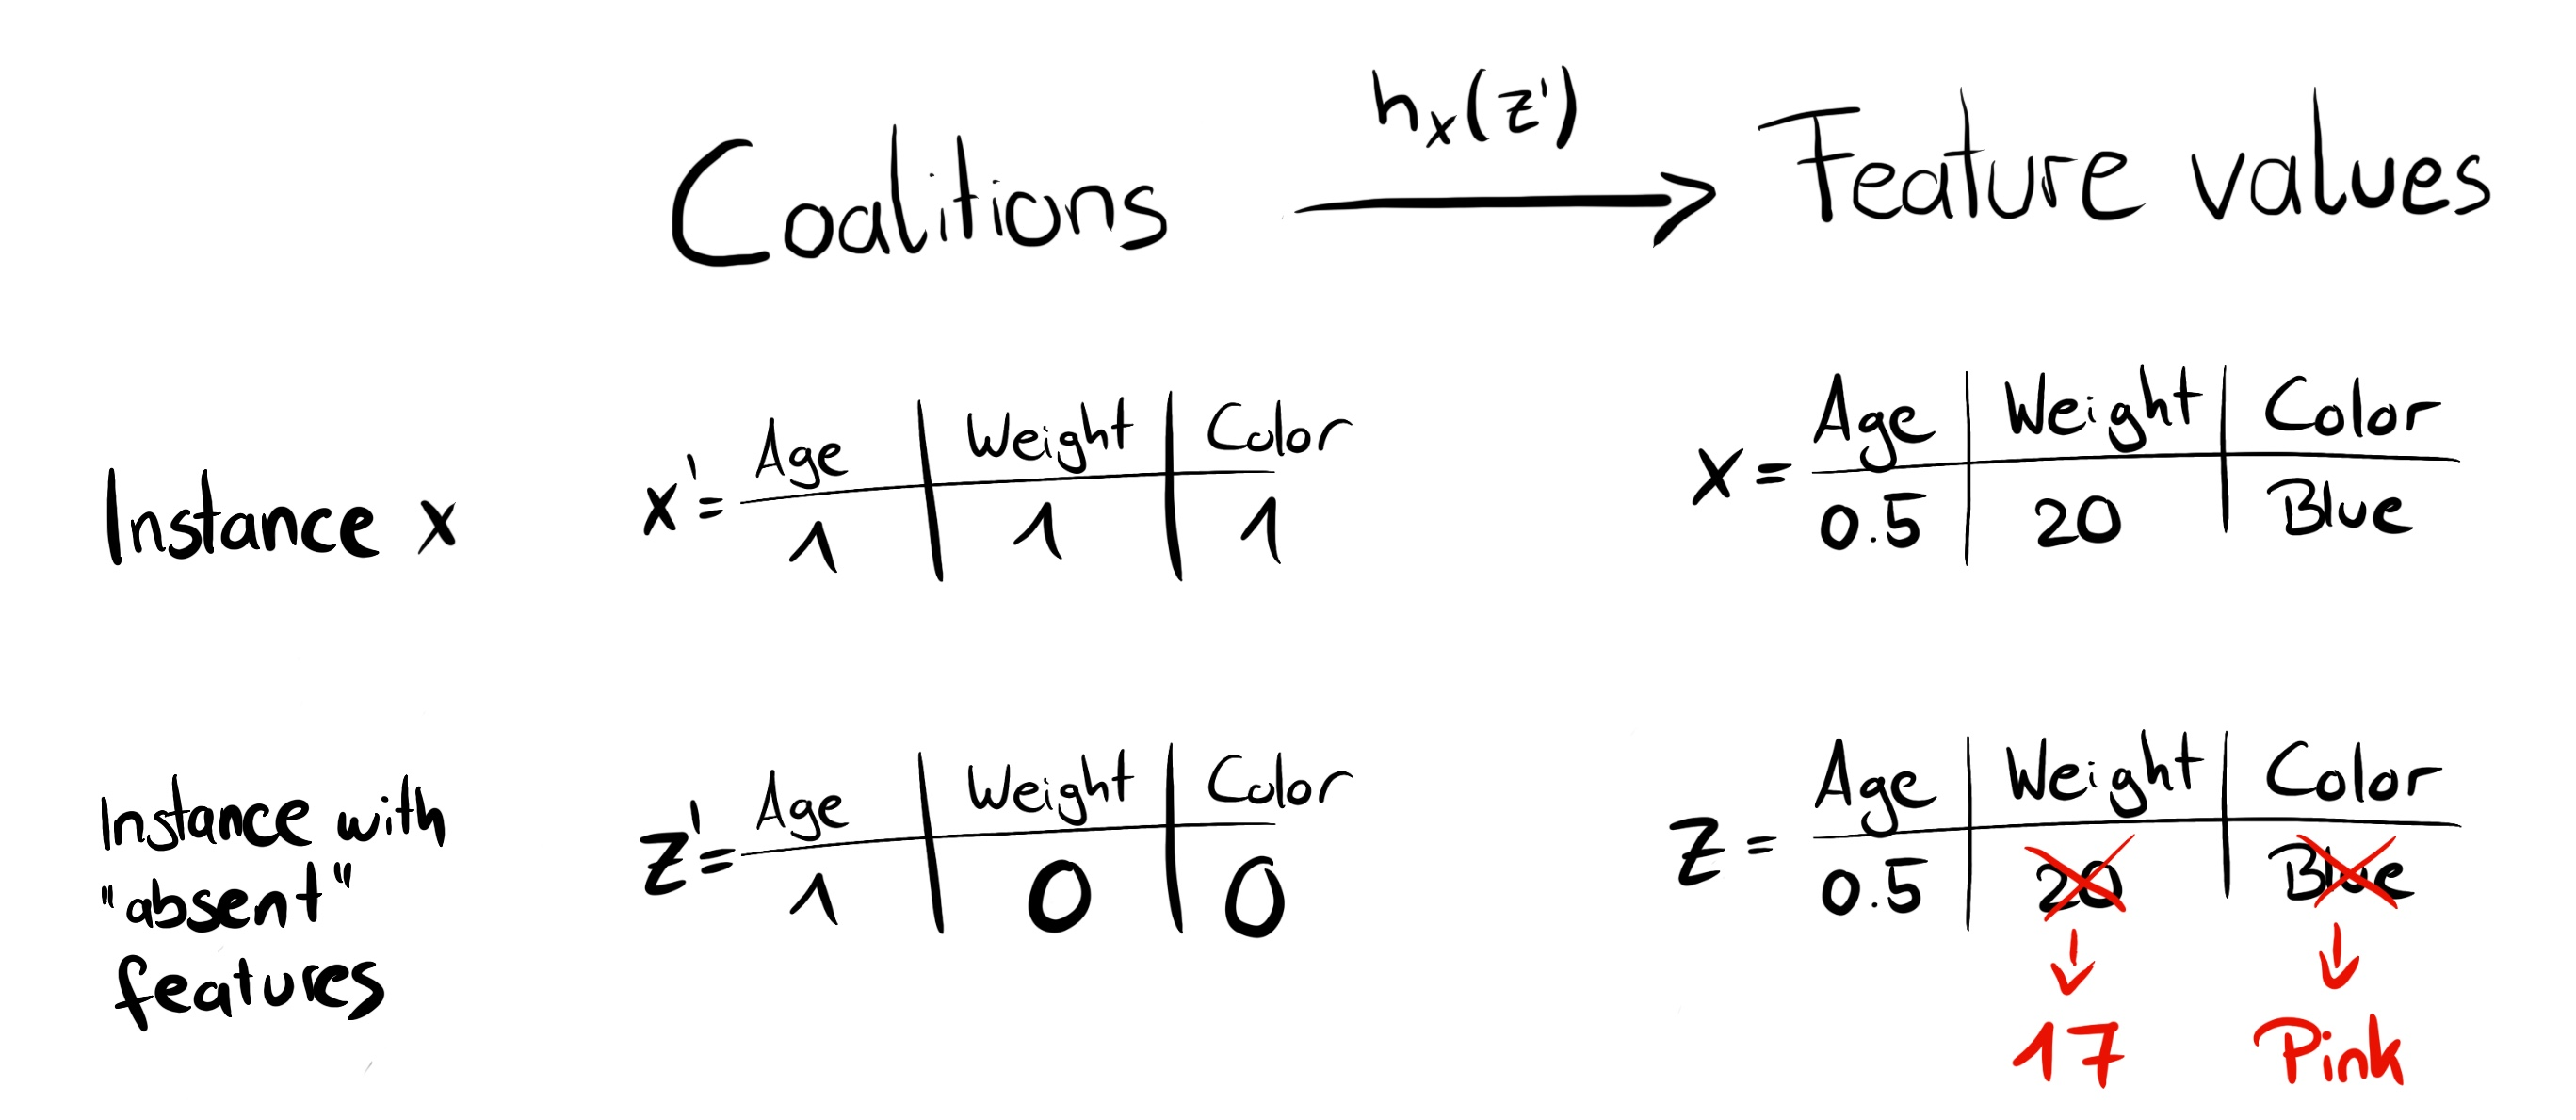
\includegraphics[scale=0.16]{images/Ch5/Sec_5.10/shap-simplified-features.jpg}
	\label{fig:5_48}
	\caption{hàm $h_x$ ánh xạ một liên minh tới một mẫu dữ liệu hợp lệ. Cho đặc trưng có mặt (1), $h_x$ ánh xạ từ các giá trị đặc trưng cũa $x$. Cho các đặc trưng vắng mặt $(0)$, ánh xạ từ các giá trị của một mẫu dữ liệu lấy mẫu ngẫu nhiên}
\end{figure*}
Hàm $h_x$ cho dữ liệu dạng bảng xử lý $X_C$ và $X_S$ độc lập và tích phân trong phân phối biên:

$$f(h_x(z'))=E_{X_C}[f(x)]$$

Lấy mẫu từ phân phối biên nghĩ là bỏ qua cấu trong phụ thuộc giữa các đặc trưng có mặt và vắng mặt. KernelSHAP do đó gặp vấn đề tương tự như tất cả các phương pháp diễn giải dự trên hoán vị. Phép ước tính đặt quá nhiều trọng số lên các mẫu dữ liệu không chắc chắn. Kết quả có thể trở nên không tin cậy. Nhưng cần thiết phải lấy mẫu từ phân phối biên. Nếu các giá trị đặc trưng vắng mặt sẽ được lấy mẫu từ phân phối có điều kiện, các giá trị kết qủa sẽ không còn là giá trị Shapley. Các kết quả sẽ vi phạm tiên đề Shapley về Nộm tính, nói rằng một đặc trưng không đóng góp lên kết quả nên có giá trị Shapley bằng $0$. 

Cho các ảnh, hình sau miêu tả một hàm ánh xạ khả thi.

\begin{figure*}[h!]
	\centering
	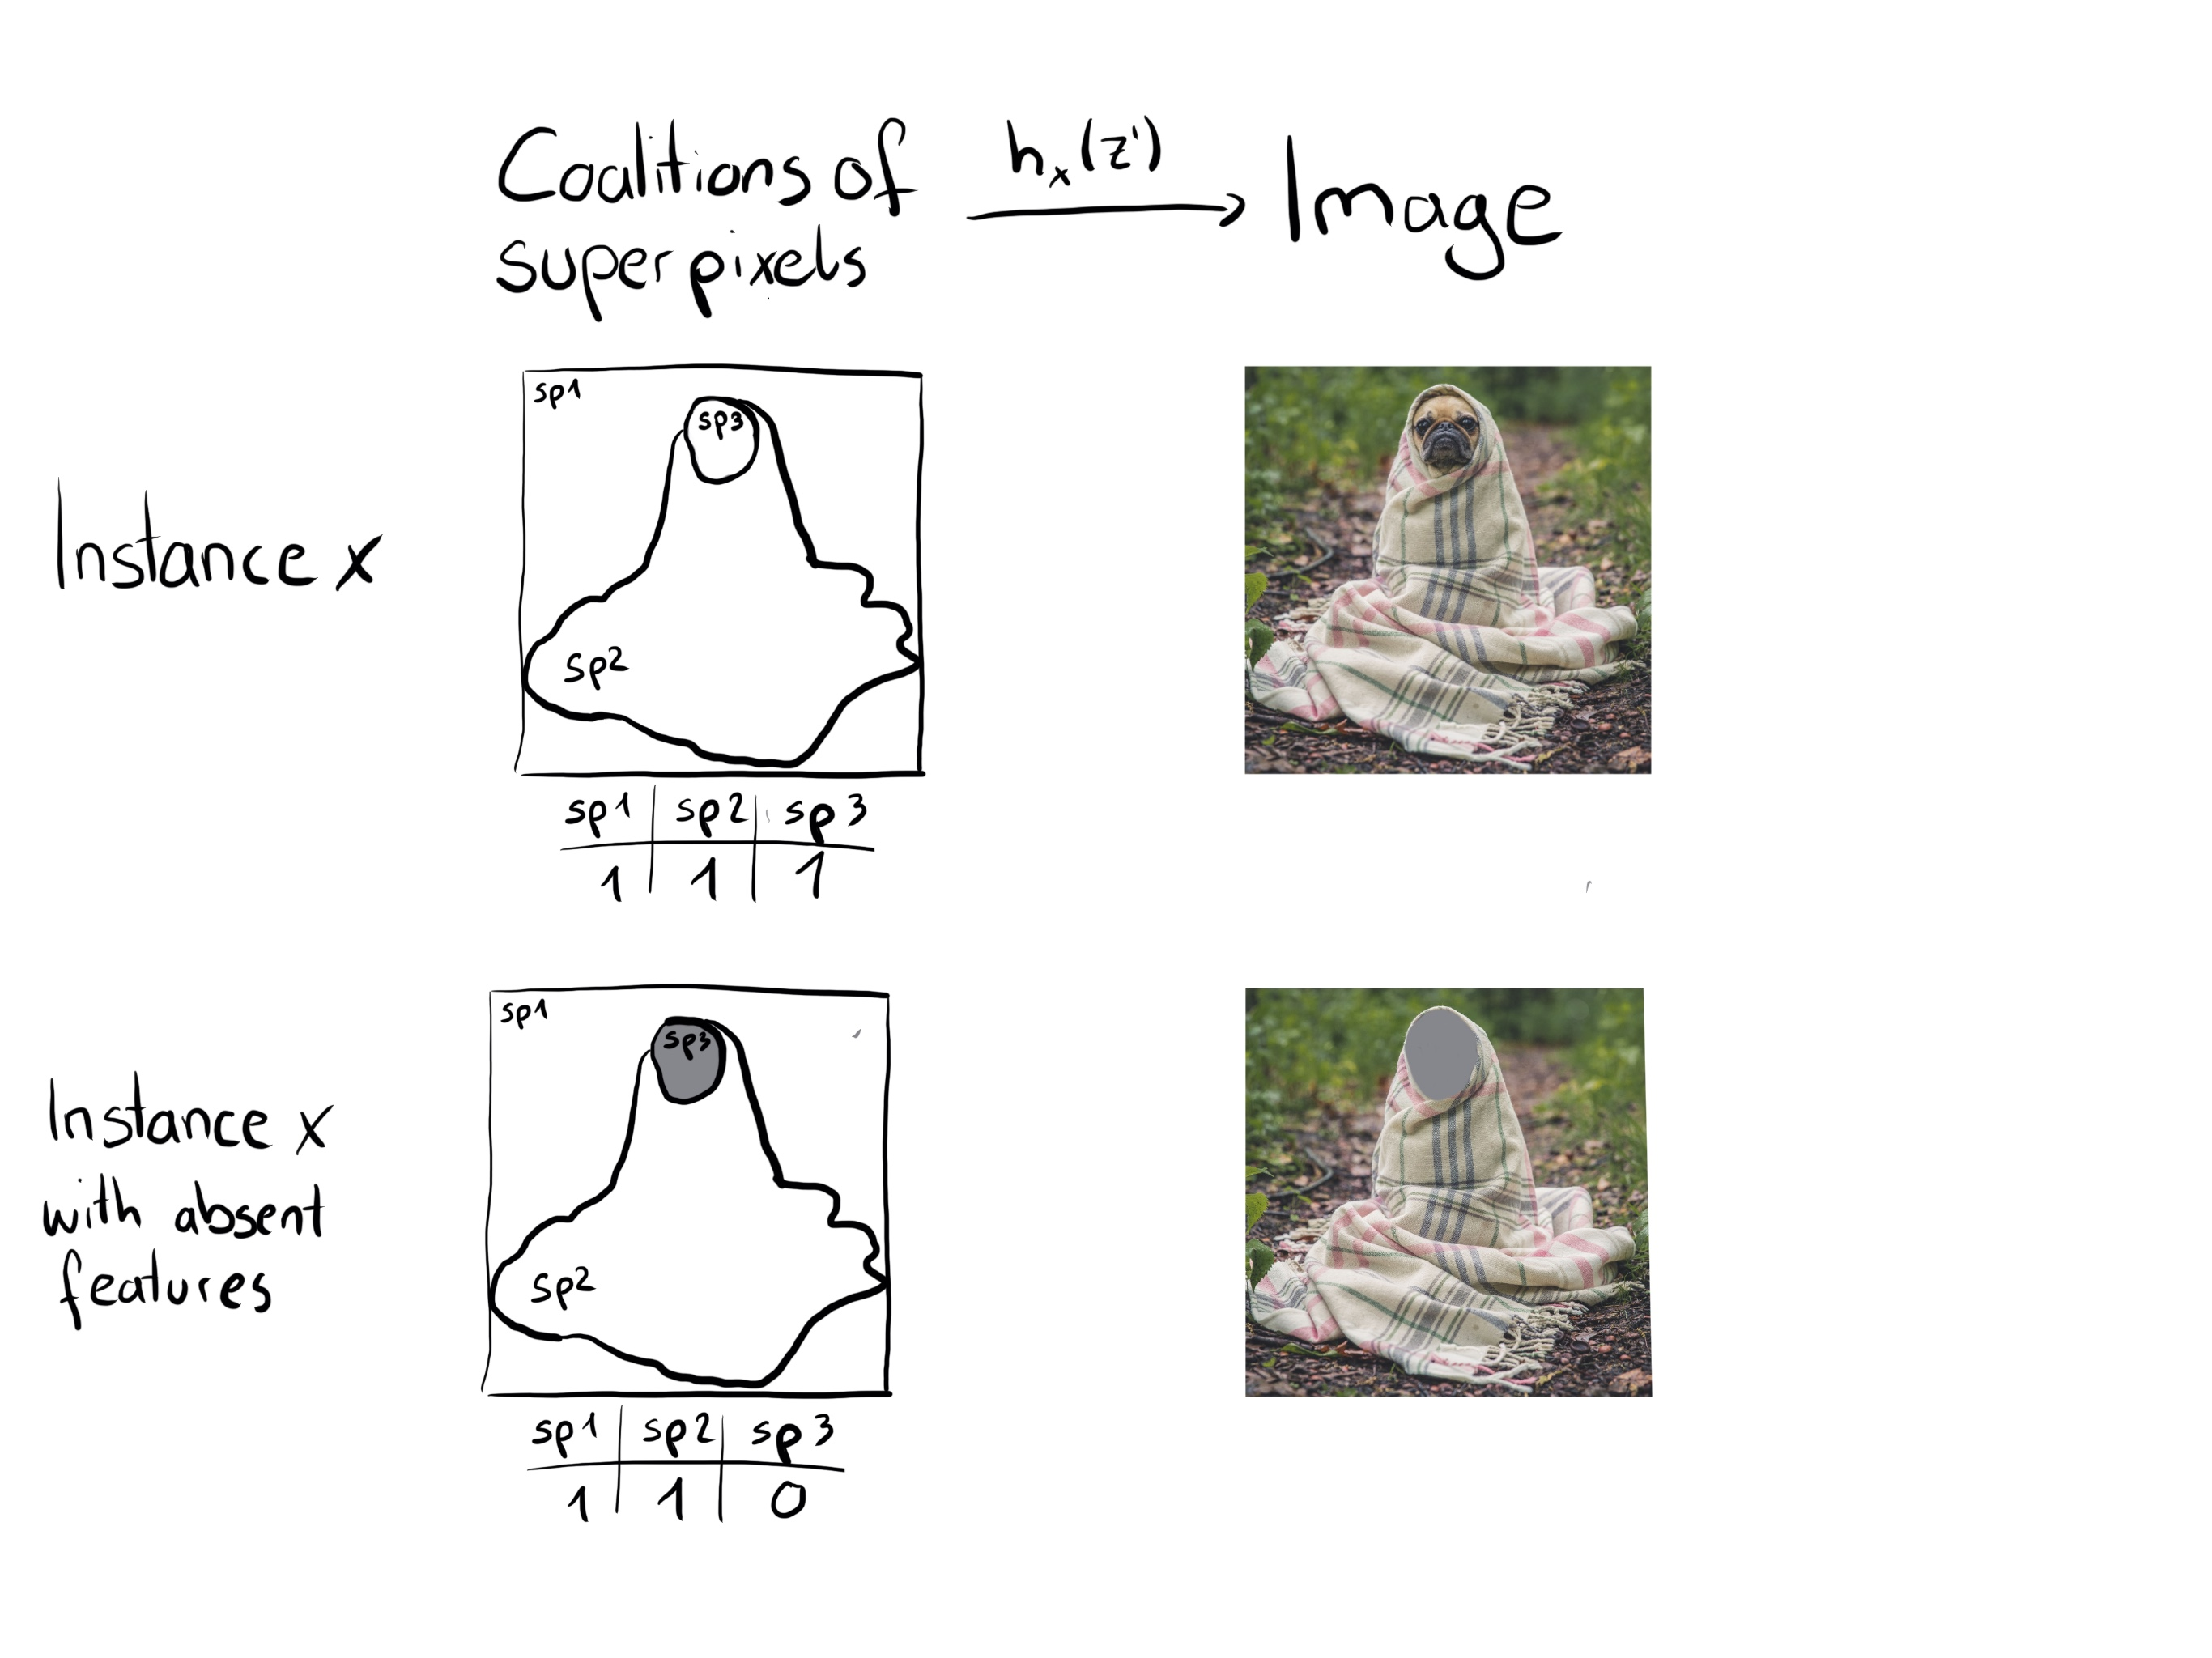
\includegraphics[scale=0.20]{images/Ch5/Sec_5.10/shap-superpixel.jpg}
	\label{fig:5_49}
	\caption{Hàm $h_x$ ánh xạ các liên minh của siêu pixels(sp) lên các ảnh. Siêu pixels là nhóm các pixels. Cho giá trị đặc trưng có mặt $(1)$,  $h_x$ trả về phần tương ứng cho ảnh gốc. Cho các giá trị đặc trưng vắng mặt $(0)$, $h_x$ làm xám đi khu vực tương ứng. Cho trung bình hoá màu của pixel xung quanh hoặc tương tự cũng là một phương án.n}
\end{figure*}

Khác biệt lớn nhất của LIME là trọng số của các mẫu dữ liệu trong mô hình hồi quy. LIME trọng số hoá các mẫu dữ liệu theo mức độ gần gũi của chúng với thể hiện ban đầu. Càng nhiều $0$ trong vector liên minh, trọng số trong LIME càng nhỏ. SHAP trọng số hoá các mẫu dự liệu được lấy mẫu dựa trên trọng lương của liên minh sẽ lấy trong ước tính giá trị Shapley. Các liên minh nhỏ (ít lượng số $1$) và liên minh lớn (nhiều lượng số $1$) có các trọng số lớn nhất. Trực giác là như sau: ta học hầu hết các đặc trưng riêng lẻ nếu chúng ta học được các ảnh hưởng (effects) một cách riêng lẻ. Nếu một liên minh chứ một đặc trưng duy nhất, ta có thể học được ảnh hưởng riêng lẻ chính của các đặc trưng lên dự đoán. Nếu một liên minh bao gồm tất cả trừ một đặc trưng, ta có thể học ảnh hưởng toàn phần của các đặc trưng này (ảnh hưởng chính cộng thêm các tương tác đặc trưng). Nếu một liên minh bào gồm nửa các đặc trưng, ta học rất ít về đóng góp từng đặc trưng riêng lẻ, vì có thể có nhiều liên minh khả thi chỉ có một nửa đặc trưng. Để đạt được trọng số tuân thủ Shapley, Lundberg et. al đề xuất hạt nhận SHAP:

$$\pi_{x}(z')=\frac{(M-1)}{\binom{M}{|z'|}|z'|(M-|z'|)}$$

Ở đây, $M$ là kích cỡ liên minh tối đa và $|z'|$ là số lượng các đặc trưng có mặt trong mấu dữ liệu $z'$. Lundberg và Lee chứng minh rằng hồi quy tuyến tính với trọng số hạt nhân này mang lại các giá trị Shapley. Nếu bạn sửa dụng hạt nhân SHAP với LIME trong dữ liệu liên minh, LIME sẽ ước lượng các giá trị Shapley!  


Chúng ta có thể khôn ngoan hơn về việc lấy mẫu các liên minh: Các liên minh nhỏ nhất và lớn nhất chiếm phần lớn trọng số. Ta thu ước lượng giá trị Shapley tốt hơn bằng các dùng một số mẫu với ngân sách $K$ (sampling budget K) để thêm vào những liên minh trọng số lớn thay vì lấy mẫu mù quáng. Chúng ta bắt đầu với mọi liên minh có thể có từ $1$ tới $M-1$ đặc trưng, tổng cộng có 2 lần liên minh $M$. Khi ta đã có đủ ngân sách còn lại (ngân sách hiện tại là $K-2M$), ta có thể kèm theo các liên minh với hai đặc trưng và với $M-2$ đặc trưng, và tiếp diễn như vậy. Từ các kích thước (size) của liên minh còn lại, ta lấy mẫu với trọng số được điều chỉnh lại.

Ta đã có dữ liệu, mục tiêu (target) và các trọng số. Mọi thứ dùng để xây dụng mô hình hồi quy tuyến tính đã trọng số hoá:

$$g(z')=\phi_0+\sum_{j=1}^M\phi_jz_j'$$

Ta huấn luyện mô hình tuyến tính $g$ qua tối ưu hoá hàm mất mát $L$: 

$$L(f,g,\pi_{x})=\sum_{z'\in{}Z}[f(h_x(z'))-g(z')]^2\pi_{x}(z')$$

Với $Z$ là dữ liệu huấn luyện. Đây là tổng sai số bình phương cũ quen thuộc mà chúng ta thường tối ưu hóa cho các mô hình tuyến tính. Các hệ số ước tính của mô hình, $\phi_j$ là các giá trị Shapley.


\subsection{TreeSHAP}

Lundberg et. al (2018) đề xuất TreeSHAP, một biến thể của SHAP cho các mô hình học máy dựa trên cây như cây quyết định, rừng ngẫu nhiên và cây tăng cường gradient (gradient boosted trees). TreeSHAP được giới thiệu là một giải pháp thay thế nhanh, theo mô hình cụ thể cho KernelSHAP, nhưng hóa ra nó có thể tạo ra các thuộc tích (attributions) về đặc trưng không trực quan.

TreeSHAP xác định hàm giá trị bằng cách sử dụng kỳ vọng có điều kiện (conditional expectation) $ E_{X_S|X_C}(f(x)|x_S)$ thay vì kỳ vọng cận biên (marginal expectation). Vấn đề với kỳ vọng có điều kiện là các đặc trưng không có ảnh hưởng lên hàm dự đoán $f$ có thể nhận ước tính TreeSHAP khác 0. Ước tính khác $0$ xảy ra khi đặc trưng tương quan với một đặc trưng khác mà gây ảnh hưởng thực sự lên dự đoán.    


TreeSHAP nhanh hơn bao nhiêu? So với KernelSHAP, nó làm giảm độ phức tạp tính toán từ $O(TL2^M)$ to $O(TLD^2)$, với $T$ là số lượng cây, $L$ là số lượng lớn nhất các lá trong một cây và $D$ là độ sâu tối đa của bất kì cây nào. 

TreeSHAP dùng kỳ vọng có điều kiện $E_{X_S|X_C}(f(x)|x_S)$ để ước lượng các ảnh hưởng. Ta sẽ cho bạn một số trực giác về các chúng ta tính kì vọng dự đoán (prediction expectation) cho một cây, một mẫu dữ liệu $x$ và một tập con đặc trưng $S$. Nếu ta điều kiện hoá tất cả các đặc trưng – nếu $S$ là tập tất cả các đặc trưng – phép đặc trưng từ một nút (node) trong đó mẫu dữ liệu $x$ nằm trong là kỳ vọng dự đoán. Nếu chúng ta không điều kiện hoá lên bất cứ đặc trưng nào – tập $S$ rỗng – ta sẽ dùng trung bình trọng số hoá (weighted average) của các dự đoán trong tất cả các nút đầu cuối (terminal nodes). Nếu $S$ chứa một số, nhưng không phải tất cả, các đặc trưng, ta bỏ qua các dự đoán của các nút không truy cập được (unreachable nodes). Không thể truy cập có nghĩa là đường quyết định (decision path) mà dẫn đến nút này mẫu thuẫn với các gía trị $x_S$. Từ các nút đầu cuối còn lại, ta trung bình các dự đoán trọng số hoá bằng kích thước các nút (tức số lượng mẫu huấn luyện trong nút đó). Trung bình của các nút đầu cuối còn lại, trọng số hoá bằng số lượng mẫu dữ liệu trên một nút, là kỳ vọng dự đoán cho $x$ với $S$ cho trước. Vấn đề ở đây là chúng ta phải áp dụng quy trình này cho mỗi tập con các gái trị đặc trưng $S$. TreeSHAP tính toán trong thời gian đa thức thay vì theo cấp số nhân (exponential). Ý tưởng cơ bản là đẩy tất cả các tập con có thể $S$ xuống cây cùng một lúc. Cho mỗi nút quyết định (decision node) ta phải theo dỏi chung số lượng các tập con. Điều này phụ thuộc vào các tập con trong nút cha-mẹ (parent node). Ví dụ khi phần tách (split) đầu tiên trong một cây là đặc trưng $x3$, mọi tập con chứa đặc trưng $x3$ đều về một nút (nút mà $x$ về). Các tập con không chứa $x3$ sẽ chuyển đến cả hai nút với trọng số giảm. Không may các tập con với kích thước khác nhau có trọng số khác nhau. Thuật toán phải theo dõi trọng số tổng thể (overall) của các tập con trong một nút. Điều này tăng phức tạp cho thuật toán. Ta để cho bài báo gốc cho chi tiết về TreeSHAP. Phép tính toán có thể mở rộng cho nhiều cây hơn: Nhờ vào Cộng tính của các giá trị Shapley, các giá trị Shapley của một nhóm cây (tree ensemble) là (trọng số) trung bình của các giá trị Shapley của các cây riêng lẽ. 

Tiếp theo, chúng ta sẽ xem xét các cách giải thích SHAP. 
\subsection{Các ví dụ:}

Ta huấn luyện một rừng ngẫu nhiên với 100 cây để dự đoán nguy cơ ung thư cổ tử cung. Chúng ta dùng SHAP để giải thích các dự đoán riêng lẽ. Ta có thể dùng phương pháp ước tính TreeSHAP nhanh hơn thay vì KernelSHAP chậm hôn, vì một rừng ngẫu nhiên là một nhóm các cây. Thay vì dựa vào các phân phối có điều kiện, ví dụ này dùng phân phối biên. ĐIều này được miêu tả trong gói thư viện mà không phải trong tài liệu gốc. Hàm Python TreeSHAP chậm hơn với phân phối biên, nhưng vẫn nhanh hơn KernelSHAP, ví nó tỉ lệ tuyến tính với số lượng hàng trong dữ liệu. 

Bởi vì chúng ta sử dụng phân phối biên ở đây, cách giải thích giống ở trong chương giá trị Shapley. Nhưng gói Python SHAP có một cách hình dung khác: bạn có thể hình dung các thuộc tính đặc trưng (feature attributions) như là các giá trị Shapley làm “các lực” (forces). Mỗi giá trị đặc trưng là một lực làm tăng hay giảm dự đoán. Dự đoán bắt đầu từ đường cơ sở (baseline). Đường cơ sở của giá trị Shapley là trung bình tất cả các dự đoán. Trong phác hoạ, mỗi giá trị Shapley là một mũi tên đẩy để tăng lên (giá trị dương) hoặc giảm đi (giá trị âm) dự đoán. Các lực này cân bằng lẫn nhau ở dự đoán thật sự của mẫu huấn luyện. 

Hình sau đây cho thấy các phác hoạ lực giải thích SHAP cho hai phụ nữ trong tập dữ liệu ung thư cổ tử cung:

\begin{figure*}[h!]
	\centering
	\includegraphics[scale=0.20]{images/Ch5/Sec_5.10/unnamed-chunk-34-1.png}
	\label{fig:5_50}
	\caption{Giá trị SHAP để giải thích dự đoán xác suất ung thư cho hai cá nhân. Đường cơ sở -- xác suất dự đoán trung bình – là 0.066. Người phụ nữ đầu có nguy cơ dự đoán thấp với 0.06. Các ảnh hưởng tăng nguy cơ như là STDs được bỳ đắp bằng các ảnh hưởng giảm như là tuổi. Người phụ nữ thứ hai có nguy cơ dự đoán cao với 0.71. Tuổi 51 và với 34 năm hút thuốc làm tăng  nguy cơ ung thư dự đoán.}
\end{figure*}

Đây là các giải thích cho các dự đoán cá nhân. 

Giá trị Shapley có thể kết hợp vào các giải thích toàn cục. Nếu ta chạy SHAP cho mỗi mẫu dữ liệu, ta có ma trận các gái trị Shapley. Ma trận này gồm một hàng mỗi mẫu dũ liệu và một cột mỗi đặc trưng. Ta có thể giải thích cả mô hình qua phân tích các giá trị Shapley trong ma trận này.

Ta bắt đầu với mức quan trọng của đặc trưng SHAP.

\subsection{Mức quan trọng của đặc trưng SHAP (SHAP feature importance)}

Ý tưởng đằng sau SHAP feature importance khá đơn giản: Các đặc trưng với gía trị tuyệt đối Shapley cao rất quan trọng. Vì chúng ta muốn mức quan trọng toàn cục (global importance), ta trung bình các giá trị tuyệt đối Shapley với mỗi đặc trưng xuyên suốt các dữ liệu:
$$I_j=\sum_{i=1}^n{}|\phi_j^{(i)}|$$
Tiếp theo, ta sắp xếp các đặc trưng giảm dần theo độ quan trọng và phác hoạ chúng. Hình dưới đây cho thấy mức quan trọng gía trị SHAP cho huấn luyện rừng ngẫu nhiên trước đó để dự đoán ung thư cổ tử cung.

\begin{figure*}[h!]
	\centering
	\includegraphics[scale=0.6]{images/Ch5/Sec_5.10/shap-importance.png}
	\label{fig:5_51}
	\caption{Mức quan trọng của đặc trưng SHAP được đo bằng trung bình giá trị tuyệt đối Shapley. Số năm sử dụng các biện pháp tránh thai nội tiết tố là đặc trưng quan trọng nhất, thay đổi xác suất ung thư tuyệt đối dự đoán trên trung bình 2.4 điểm phần trăm (0.024 trên trục x).}
\end{figure*}

Mức quan trọng của đặc trưng SHAP là một thay thế cho tầm quan trọng của đặc trưng hoán vị. Có một sự khác biệt lớn giữa cả hai mức đo độ quan trọng (important measures): Mức quan trọng của đặc trưng hoán vị dựa trên sự giảm hiệu suất của mô hình. SHAP dựa trên mức của các thuộc tính đặc trưng (feature attributions).

Đồ thị mức quan trọng đặc trưng hữu ích, nhưng không chứa thông tin khác ngoài các mức quan trọng.



\subsection{Phác hoạ tổng quan SHAP (SHAP Summary Plot)}

Phác hoạ tổng quan kết hợp mức quan trọng với các ảnh hưởng đặc trưng. Mỗi điểm trong phác hoạ tổng quan là một giá trị Shapley cho một đặc trưng và một mẫu dữ liệu. Vị trí trên trục y được quyết định bởi đặc trưng và trên trục x qua giá trị Shapley. Màu thể hiện giá trị của đặc trưng từ thấp tới bé. Các điểm chồng (overlapping points) lộn xộn ở hướng trục y, nên ta hiểu được phân phối của các giá trị Shapley trên mỗi đặc trưng. Các đặc trưng được sắp xếp theo mức quan trọng của chúng.  

\begin{figure*}[h!]
	\centering
	\includegraphics[scale=0.6]{images/Ch5/Sec_5.10/shap-importance-extended.png}
	\label{fig:5_52}
	\caption{Phác hoạ tổng quan SHAP. Ít năm dùng các biện pháp tránh thai nội tiết tố thì giảm nguy cơ ung thư dự đoán, nhưng nhiều năm hơn thì sẽ tăng nguy cơ. Các ảnh hưởng thường mô tả hành vi của mô hình và không nhất thiết phải thông dụng trong thế giới thực.}
\end{figure*}

Trong phác hoạ tổng quan, chúng ta thấy những dấu hiệu đầu tiên về mối quan hệ của một đặc trưng và ảnh hưởng lên dự đoán. Nhưng để thấy hình thức chính xác của mối quan hệ này, ta phải nhìn qua các phác hoạ phụ thuộc SHAP.

\subsection{Các phác hoạ phụ thuộc SHAP (SHAP Dependence Plot)}

Các phác hoạ phụ thuộc SHAP có thể là phác hoạ giải thích toàn cục đơn giản nhất (simplest global intepretation plot): 1) Chọn một đặc trưng. 2) VỚi mỗi mẫu dữ liệu, phác hoạ một điểm với giá trị đặc trưng trên trục x và giá trị Shapley tương ứng trên trục y. 3) Đã xong. 

Về mặt toán học, phác hoạ chứa các điểm sau:  $ \{(x_j^{(i)},\phi_j^{(i)})\}_{i=1}^n$
. Hình sau cho thấy sự phụ thuộc đặc trưng SHAP trong nhiều năm vào các biện pháp tránh thai nội tiết tố:

\begin{figure*}[h!]
	\centering
	\includegraphics[scale=0.9]{images/Ch5/Sec_5.10/shap-dependence.png}
	\label{fig:5_53}
	\caption{Phác hoạ phụ thuộc riêng SHAP cho nhiều năm vào các biện pháp tránh thai nội tiết tố. So với $0$ năm, một vài năm làm thấp hơn xác suất dự đoán và số năm làm tăng xác suất ung thư dự đoán. }
\end{figure*}

Các phác hoạ phụ thuộc SHAP là thay thế cho phác hoạ phụ thuộc riêng (PDP) và các phác họa tích lũy ảnh hưởng cục bộ (ALE). Trong khi PDP và ALE cho thấy các ảnh hưởng trung bình, phác hoạ phụ thuộc SHAP cũng cho thấy phương sai trên trục y. Đặc biệt trong trường hợp tương tác, phác hoạ phụ thuộc SHAP sẽ phân tán nhiều hơn trong trục y. Phác hoạ phụ thuộc có thể cải thiện bằng cách làm nổi bật các tương tác đặc trưng. 

\subsection{Giá trị tương tác SHAP (5.10.8 SHAP Interaction Values):}

Ảnh hưởng tương tác (interaction effect) là ảnh hưởng đặc trưng kết hợp bổ sung (additional combined feature effect) sau khi tính đến các hiệu ứng đặc trưng riêng lẻ. Chỉ số tương tác Shapley (Shapley interaction index) từ lý thuyết trò chơi được định nghĩa là: 
$$\phi_{i,j}=\sum_{S\subseteq\setminus\{i,j\}}\frac{|S|!(M-|S|-2)!}{2(M-1)!}\delta_{ij}(S)$$
Với $i \neq j$ và: 
$$\delta_{ij}(S)=f_x(S\cup\{i,j\})-f_x(S\cup\{i\})-f_x(S\cup\{j\})+f_x(S)
$$
Công thức này trừ đi ảnh hưởng chính của các đặc trưng khi tính đến các ảnh hưởng riêng lẻ để thu được ảnh hưởng đặc trưng thuần tuý. Ta lấy trung bình tất cả khác liên minh đặc trưng có thể $S$, như trong phép tính giá trị Shapley. Khi ta tính các giá trị tương tác SHAP cho tất cả đặc trưng, ta thu về một đặc trưng trên một mẫu dữ liệu với kích thước $M \times M$, với $M$ là số lượng các đặc trưng.

\begin{figure*}[h!]
	\centering
	\includegraphics[scale=0.90]{images/Ch5/Sec_5.10/shap-dependence-interaction.png}
	\label{fig:5_54}
	\caption{Phác hoá phụ thuộc đặc trưng SHAP với tương tác trực quan hoá. Nhiều năm dùng biện pháp tránh thai nội tiết tố có tương tác với STDs. Trong những trường hợp gần với $0$ năm, sự xuất hiện của STD làm tăng nguy cơ ung thư dự đoán. Một lần nữa, đây không phải mô hình nhân quả. Các hiệu ứng có thể do nhiễu rối (confounding) (ví dụ STDs và nguy cơ ung thư thấp có thể tương quan với đi khám bác sĩ nhiều hơn).}
\end{figure*}

Đây là các phác hoạ ``lực'' (force plots), với mỗi phác hoạ giải thích dự đoán trên một mấu dữ liệu. Ta xoay các biểu đồ lực theo chiều dọc và đặt chúng cạnh nhau theo như sự giống nhau từ phân cụm. 

\begin{figure*}[h!]
	\centering
	\includegraphics[scale=0.40]{images/Ch5/Sec_5.10/shap-clustering.png}
	\label{fig:5_55}
	\caption{Các giải thích SHAP chồng lên nhau được phân cụm theo tính \textbf{tương đồng khi khả giải thích}. Mỗi vị trí trên trục x là một mẫu dữ liệu của dữ liệu. Giá trị SHAP màu đỏ làm tăng dự đoán, giá trị màu xanh làm giảm dự đoán. Có một cụm nổi bật: Bên phải là một nhóm có nguy cơ ung thư dự đoán cao.}
\end{figure*}
\subsection{Ưu điểm}

Vì SHAP tính toán các giá trị Shapley nên nó có tất cả các ưu điểm của Shapley: SHAP có \textbf{nền tảng lý thuyết vững chắc} trong lý thuyết trò chơi. Dự đoán được \textbf{ phân phối công bằng} giữa các giá trị đặc trưng. Ta thu được các giải thích trái ngược nhau (contrasive explanantions) mà so sánh dự đoán với trung bình dự đoán. 

SHAP \textbf{kết nối LIME và các giá trị Shapley}. Điều này rất cần thiết để hiểu thêm cả hai phương pháp. Điều này giúp thống nhất ngành học máy khả giải thích.

SHAP \textbf{triển khai nhanh chóng cho cách mô hình dựa trên cây}. Ta tin rằng đây là chìa khoá cho sự phổ biến của SHAP, vì rào cản lớn nhất cho áp dụng các giá trị Shapley là sự tính toán chậm. 

Việc tính toán nhanh giúp khả thi việc tính nhiều các giá trị Shapley cần thiết cho \textbf{các diễn giải mô hình toàn cục} (global intepretation models). Các phương pháp diễn giải toàn cục gồm mức quan trọng của đặc trưng, tính phụ thuộc đặc trưng, các tương tác, phân cụm và các phác hoạ tổng quan, vì các giá trị Shapley là “đơn vị nguyên tử” cho các diễn giải toàn cầu. Nếu bạn dùng LIME cho giải thích cục bộ và phác hoạ phụ thuộc riêng chung với mức quan trọng hoán vị đặc trưng cho giải thích toàn cục, bạn đã thiếu nền tảng chung.

\subsection{Nhược điểm}
\textbf{KernelSHAP chậm}. Điều này làm KernelSHAP phi thực tế khi bạn muốn tính toán giá trị Shapley cho nhiều điểm dữ liệu. Ngoài ra các phương pháp SHAP toàn cục như là mức độ quan trọng đặc trưng SHAP yêu cầu tính các gía trị Shapley cho rất nhiều điểm dữ liệu.

\textbf{KernelSHAP bỏ qua sự phụ thuộc đặc trưng}. Hầu hết các phương pháp diễn giải dự trên hoán vị có vấn đề này. Qua thay đổi các giá trị đặc trưng với các giá trị từ các mẫu dự liệu ngẫu nhiên, thường sẽ dễ hơn để lấy mẫu ngẫu nhiên từ phân phối biên. Tuy nhiên, nếu các đặc trưng phụ thuộc, tức tương quan, điều này dẫn đến đặt quá nhiều trọng số lên các điểm dữ liệu không khả thi. TreeSHAP giải quyết vấn đề này qua mô hình hoá cụ thể dự đoán kỳ vọng có điều kiện.

\textbf{TreeSHAP có thể tạo ra các thuộc tính đặc trưng không trực quan}. Khi TreeSHAP giải quyết vấn đề ngoại suy (extrapolating) tới các điểm dữ liệu không khả thi, nó thêm vào một vấn đề mới. TreeSHAP thay đổi hàm giá trị bằng cách dựa vào dự đoán kỳ vọng có điều kiện. Thay đổi hàm giá trị làm các đặc trưng mà không ảnh hưởng lên dự đoán có thể nhận giá trị TreeSHAP khác 0.

Những nhược điểm của giá trị Shapley cũng áp dụng cho SHAP: Giá trị Shapley có thể bị hiểu sai và cần có quyền truy cập dữ liệu để tính toán chúng cho dữ liệu mới (ngoại trừ TreeSHAP).

\subsection{Phần mềm và các gói thay thế}

Các tác giả đã triển khai SHAP trong gói Python \href{https://github.com/slundberg/shap }{shap}. Việc triển khai này hoạt động với các mô hình dựa trên cây trong thư viện học máy \href{ https://scikit-learn.org/stable/ }{scikit-learn} cho Python. Gói shap cũng được dùng cho các ví dụ trong chương này. SHAP được tích hợp vào các cơ chế tăng cường cây \href{ https://github.com/dmlc/xgboost/tree/master/python-package }{xgboost} và \href{ https://github.com/microsoft/LightGBM }{LightGBM}. Trong R có các gói \href{ https://modeloriented.github.io/shapper/}{shapper} và \href{https://github.com/bgreenwell/fastshap}{fastshap}. SHAP cũng được bao gồm trong gói R \href{ https://rdrr.io/cran/xgboost/man/xgb.plot.shap.html }{xgboost}.

\end{enumerate}

\clearpage